\documentclass[dvipdfmx]{jsreport}

% 枠
\usepackage{fancybox}
\usepackage{ascmac}
% 色
\usepackage{color}
% 数式
\usepackage{amsmath}
\usepackage{amsfonts}
\usepackage{mathtools}
\usepackage{bm,physics}
\usepackage{siunitx}
\usepackage[thicklines]{cancel}
% 画像
\usepackage[dvipdfmx]{graphicx} % 画像出力をする.
% \usepackage[draft]{graphicx} % 画像出力を枠だけにする.
\usepackage[hang,small,bf]{caption}
\usepackage[subrefformat=parens]{subcaption}
\usepackage{wrapfig} % 文字の回り込み用のパッケージ.
\usepackage{here}
% グラフ
\usepackage{tikz}
\usetikzlibrary{
  intersections,
  calc,
  arrows.meta
}
% ソースコード
\usepackage{listings,jlisting}
\lstset{
  language=C++,
	stringstyle={\ttfamily},
	commentstyle={\ttfamily},
	basicstyle={\ttfamily},
	columns=fixed,
  frame={tb},
  breaklines=true,
  columns=[l]{fullflexible},
	backgroundcolor=\color[gray]{.90}, % pdfをコピペしたときに行番号を巻き込まないようにする.
  numbers=left, % 行数を表示したければonにする.
  xrightmargin=0em,
  xleftmargin=3em,
  numberstyle={\scriptsize},
  stepnumber=1,
  numbersep=1em,
	tabsize=2,
  lineskip=-0.5ex
}
% アンカー
\usepackage[dvipdfmx]{hyperref}
\usepackage{pxjahyper}
\hypersetup{
  setpagesize=false,
  bookmarksnumbered=true,
  bookmarksopen=true,
  colorlinks=true,
  linkcolor=blue,
  citecolor=red,
  urlcolor=magenta
}
% 数式相互参照
\usepackage{cleveref}
\usepackage{autonum}
\numberwithin{equation}{subsection}


\begin{document}

% 表紙
\title{\href{https://github.com/m-agnet/Report.git}{壁の濡れ性から誘起される非平衡流体系のダイナミクスの変化}}
\author{20S2035Y 山本 凜 \thanks{茨城大学 理学部理学科物理学コース 物性理論グループ 中川研究室}}
\date{最終更新日: \today}
\maketitle

\newpage
% 目次
\setcounter{tocdepth}{3}
\tableofcontents
\newpage
% 本文

\addcontentsline{toc}{chapter}{概要}
\chapter*{概要}

やかんに火をかけて, 湯を沸かすときのことを考えてほしい. やかんのフタには蒸気を逃すために穴が空いているが, それを塞ぐと, やかんの底よりも冷たいフタの裏に細かい水滴が付き, ある程度集まって塊となったらその水滴がポチャンと落ちる様子が想像できるだろう.
先行研究によると, フタの裏に強い濡れ性を与えると, 流体系は非定常で周期的なダイナミクスを示すことが分かっている.
これは, 「フタの裏付近での水蒸気形成, フタへの水の吸着, そして水の落下」を繰り返すというものである. 
本研究では, 例にやかんを使うと, 内部の水がフタの裏に引っ付いたり, 落ちたりということを繰り返すことに対して興味を持ち, 数値実験を用いて, その繰り返しに周期性があるか, そのフタの性質によって繰り返しの仕方に変化が生まれるかを調べた. 

\begin{figure}[H]
    \centering
    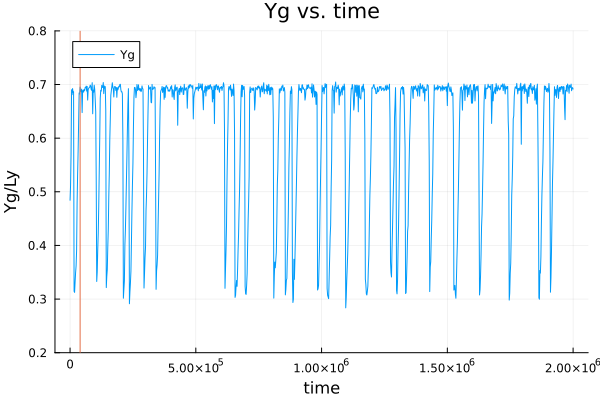
\includegraphics[scale=0.5]{/Users/2023_2gou/Desktop/r_yamamoto/Report/image/RaRtmap10_cycle/2023-12-28T12:38:52.986_map_10times_chi1.265_Ay50_rho0.4_T0.43_dT0.04_Rd0.0_Rt0.5_Ra1.877538_g0.0003999718779659611_run4.0e8.png}
    \caption{}
    \label{fig: cycle}
\end{figure}

具体的には, 上下に濡れた壁がつき, 下向きに重力がかかり, 温度差をつけた熱浴を上下に設定することで, 上向きに熱流を流すことを考えた流体系を設計した. 
ただし, 重力の強さと熱流の大きさを特徴づけるパラメータ $mgL_y$ と $k_{\text{B}}\Delta T$ の比を1程度としている. 
壁の濡れ性をパラメータ制御して, 分子動力学計算を用いて数値実験を行い, 系の重心位置と空間的なばらつきに焦点を当てて分析すると, 周期的なダイナミクスが現れる系では, 両者は相空間上で比較的安定した半円の閉軌道を描くことが分かった.$(図\ref{fig: cycle})$
さらに, 壁の濡れ性を強くしたときに, 周期的なダイナミクスがより顕著に現れることも明らかになった. 

\chapter{系の設定}

この章では, 本研究で扱う系の設定について説明する. 

2次元の気液共存系で, 質量$m$の粒子が$N$個存在することを考え, 系の上下には壁, 左右には周期境界条件を課す. また, 重力を$y$軸負の向きにかけて, 熱流を$y$軸正の向きに流す. この熱流は, 系の上下の領域にそれぞれ異なる温度を設定したlangevin熱浴を使用することによってかけることとし, NVT-MDシミュレーションを実行する. また, 各熱浴の$y$幅は$8\sigma$となるように設定する. (図\ref{fig:system})


\begin{figure}[H]
  \centering
  \caption{}
  \label{fig:system}
  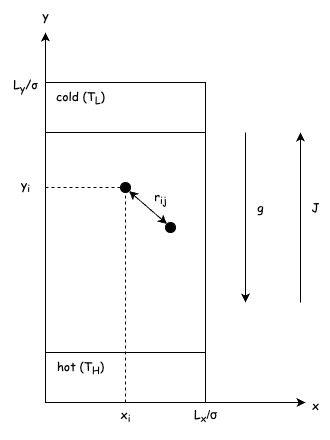
\includegraphics[scale=0.7]{image/system.jpg}
\end{figure}

\section{ハミルトニアン}

\begin{align}
  \label{Hamiltonian}
  H(\Gamma; g)
  &= \sum_{i=1}^{N}
  \left[
    \frac{{\bm{p}_i}^2}{2m} 
    + \sum_{j > i}^{N}
      \tilde{\phi}_{\text{LJ}}^{\text{pair}}(r_{ij})
    + mgy_i
    + V^{\text{wall}} (y_i)
  \right] 
\end{align}

第1項から第4項まで順に, 運動エネルギー, 粒子-粒子間相互作用ポテンシャル, 重力ポテンシャル, 壁-粒子間相互作用ポテンシャルである. 以降, 本節はこのハミルトニアンに至るまでの過程を述べる.

\subsection{粒子-粒子間相互作用ポテンシャル}

シミュレーションを行う際に, 典型的な粒子間相互作用ポテンシャルとして, 12-6 Lennard-Jones Potential を採用する.

\begin{align}
  \phi_{\text{LJ}}^{\text{pair}}(r; \varepsilon, \sigma) = 4\varepsilon \qty[\qty(\frac{\sigma}{r})^{12} - \qty(\frac{\sigma}{r})^{6}] 
\end{align}

シミュレーション上では, カットオフ長 $r_{\text{cut}}^{\text{pair}}=3\sigma$ とポテンシャルのシフトアップを考慮して

\begin{align}
  \tilde{\phi}_{\text{LJ}}^{\text{pair}}(r;r_{\text{cut}}^{\text{pair}}) = \qty{\phi_{\text{LJ}}^{\text{pair}}(r) - \phi_{\text{LJ}}^{\text{pair}}(r_{\text{cut}}^{\text{pair}})}\theta \qty(r_{\text{cut}}^{\text{pair}}-r) \\
\end{align}

のように書き換えたポテンシャルを用いている.

\subsection{周期境界条件と最近接イメージ規約}

周期境界条件を考慮すると, 粒子-粒子間相互ポテンシャルの総計はまず以下のように書ける.\cite{MD}

\begin{align}
  \sum_{n_x \in \mathbb{Z}} \sum_{i=1}^{N} \sum_{\substack{j=1 \\ (j \neq i \ \text{for} \ n_{x} = 0)}}^{N} \frac{1}{2} \phi_{\text{LJ}}^{\text{pair}}(|\bm{r}_i -(\bm{r}_j + L_x \bm{e}_x)|) 
\end{align}

ここで, $n_x = 0$; オリジナルセルの中では, 同じ$i,\ j$ペアのポテンシャルエネルギーを2回足すことになるので, ポテンシャルを$1/2$している. その上で, $j = i$の場合は自分自身との相互作用になるため, これは除外する. $n_x \neq 0$の場合, 粒子$j$はイメージ粒子となるため, $j=i$の場合も含めることになる. このときにもダブルカウントがあるので, ポテンシャルを$1/2$している. 

\begin{figure}[H]
  \centering
  \caption{}
  \label{fig:system_periodic}
  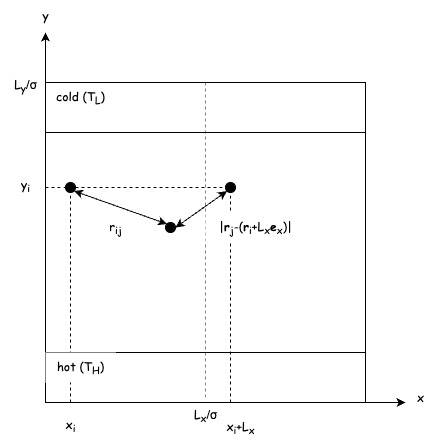
\includegraphics[scale=0.7]{image/system_periodic.jpg}
\end{figure}

注目する系の粒子が常にオリジナルセルの中にとどまっているかのようにMD上で扱うには,

\begin{align}
  x_{i} = x_{i}' \mod L_{x} 
\end{align}

のように,  飛び出した粒子の$x$座標$x_{i}'$を上式のように$x_i$にシフトすれば良い. しかし, 周期境界条件とセットに, 最近接イメージ規約として, 粒子$i$がオリジナル粒子と各イメージ粒子の中で最も近い粒子$j$らとのみ相互作用をすることを課すと, 粒子間の相互ポテンシャルの総計は先ほどよりも簡単に書けるようになる.

\begin{align}
  \sum_{i=1}^{N} \sum_{j > i}^{N} \phi_{\text{LJ}}^{\text{pair}} (r_{ij})
\end{align}

\subsection{壁-粒子間相互作用ポテンシャル}

\begin{align}
  \phi_{\text{LJ}}^{\text{wall}}(r; \varepsilon^{\text{wall}}, \sigma^{\text{wall}}) = 4\varepsilon^{\text{wall}} \qty[\qty(\frac{\sigma^{\text{wall}}}{r})^{12} - \qty(\frac{\sigma^{\text{wall}}}{r})^{6} ] \\
\end{align}

パラメータは以下のようにする.

\begin{align}
  \varepsilon^{\text{wall}} &= \qty(1.0 - \text{R}_\text{d}) \times \varepsilon \\
  \sigma^{\text{wall}} &= \qty(0.5 + \text{R}_\text{t}) \times \sigma \\
  r^{\text{wall}}_{\text{cut}} &= \qty(2^{1/6} + \text{R}_\text{a}) \times \sigma^{\text{wall}}
\end{align}

カットオフ長とシフトアップを考慮して

\begin{align}
  \tilde{\phi}_{\text{LJ}}^{\text{wall}}(r;r_{\text{cut}}^{\text{wall}}) = \qty{\phi_{\text{LJ}}^{\text{wall}}(r) - \phi_{\text{LJ}}^{\text{wall}}(r_{\text{cut}}^{\text{wall}})}\theta \qty(r_{\text{cut}}^{\text{wall}}-r) \\
\end{align}

この系では, $y=0$と$y=L_y$に壁がついている. よって, 壁ポテンシャルは

\begin{align}
  V^{\text{wall}}(y; L_y) &= \tilde{\phi}_{\text{LJ}}^{\text{wall}}(y;r_{\text{cut}}^{\text{wall}}) + \tilde{\phi}_{\text{LJ}}^{\text{wall}}(L_y - y;r_{\text{cut}}^{\text{wall}})
\end{align}

のように書ける. これまでのことより, ハミルトニアンは式\eqref{Hamiltonian}のように書き表せる.

\begin{align}
    H(\Gamma; g)
    &= \sum_{i=1}^{N}
    \left[
      \frac{{\bm{p}_i}^2}{2m} 
      + \sum_{j > i}^{N}
        \tilde{\phi}_{\text{LJ}}^{\text{pair}}(r_{ij})
      + mgy_i +V^{\text{wall}}(y_i)
    \right] \ \tag*{\eqref{Hamiltonian}} 
\end{align}

\section{熱流}

熱伝導系はランジュバン熱浴を設計することで

粒子$i$が熱浴に侵入すると, その粒子の運動はランジュバン方程式に従う. 侵入していないときは, $\gamma = 0$になり, 正準方程式に等しくなる.

\begin{align}
  \dot{\bm{r}_i} &= \pdv{H}{\bm{p}_i} \\
  \dot{\bm{p}_i} &= - \pdv{H}{\bm{r}_i} - \gamma \dot{\bm{r}_i} + \sqrt{2 \gamma k_{\text{B}}T_{\nu}}\bm{\xi}_i (t) 
\end{align}

\begin{align}
  \expval{\xi_{i}^{a}(t)} &= 0 \\
  \expval{\xi_{i}^{a}(t)\xi_{j}^{b}(t')} &= \delta_{i,j} \delta_{a,b}\delta (t-t')
\end{align}

\begin{align}
  \gamma(y_i) &= 1. \ T_{\nu}(y_i) = T_{\text{H}}. \ (0 < y_i < 8\sigma) \\
  \gamma(y_i) &= 1. \ T_{\nu}(y_i) = T_{\text{L}}. \ (L_y - 8\sigma < y_i < L_y) \\
  \gamma(y_i) &= 0.  \ (8\sigma < y_i < L_y - 8\sigma)
\end{align}

\chapter{数値実験の結果}\label{chap:simulation}

この章では, 行ったシミュレーションの設定についてそれぞれ説明をして, その結果得た各系の重心位置の推移を示す.

以下のように, $\text{R}_\text{a}$と$\text{R}_\text{t}$を少しずつ変えた系を設定して, 25種類の系でそれぞれシミュレーションをした. これ以降, 簡単のために各系のことをそれぞれの図のキャプションに示されたアルファベットを用いて示すことがある. 例えば, 25個の系を用意した場合は表 \ref{tb:system} のように呼ぶことがある. 

\vspace{1\baselineskip}

\begin{table}
  \centering
  \begin{tabular}{|c|c|c|c|c|c|} \hline
          & $\text{R}_\text{a}:0.0$ & $\text{R}_\text{a}:0.4693$ & $\text{R}_\text{a}:0.9387$ & $\text{R}_\text{a}:1.408$ & $\text{R}_\text{a}:1.877$ \\ \hline
    $\text{R}_\text{t}:0.0$ & a      & b      & c      & d      & e     \\ \hline
    $\text{R}_\text{t}:0.125$ & f      & g      & h      & i      & j     \\ \hline
    $\text{R}_\text{t}:0.25$ & k      & l      & m      & n      & o     \\ \hline
    $\text{R}_\text{t}:0.375$ & p      & q      & r      & s      & t     \\ \hline
    $\text{R}_\text{t}:0.5$ & u      & v      & w      & x      & y     \\ \hline
  \end{tabular} 
  \caption{}
  \label{tb:system}
\end{table}

\section{重力と熱流を同時にかける}\label{sec:RaRtmap}

\vspace{1\baselineskip}

まずは, 重力と熱流を同じタイミングでかけたシミュレーションを用意した. 粒子数は1250個にして, その他のパラメータについては先行研究\cite{Yoshida}を参考にした. 

\begin{itemize}
  \item $N = 1250$
  \item $\rho {\sigma}^2 = 0.4$
  \item $L_x / \sigma \simeq 39.5$
  \item $L_y / \sigma \simeq 79.0$
  \item $k_{\text{B}} T / \varepsilon = 0.43$
  \item $k_{\text{B}} \Delta T / \varepsilon = 0.04$
  \item $mg\sigma/\varepsilon \simeq 4.0 \times 10^{-4}$
  \item $_i \sqrt{\varepsilon / m \sigma^2}= 4.0 \times 10^4$
  \item $t_f \sqrt{\varepsilon / m \sigma^2} = 2.0 \times 10^{5}$
\end{itemize}

図\ref{fig:RaRtmap_movie}で定常状態($t\sqrt{\varepsilon / m \sigma^2} = 2.0 \times 10^{5}$)時点でのスナップショットを見る.

\begin{figure}[H]
  \begin{tabular}{ccccc}
    \begin{minipage}[t]{0.2\hsize}
      \centering
      \href{https://youtu.be/yc-GeIQBuCk}{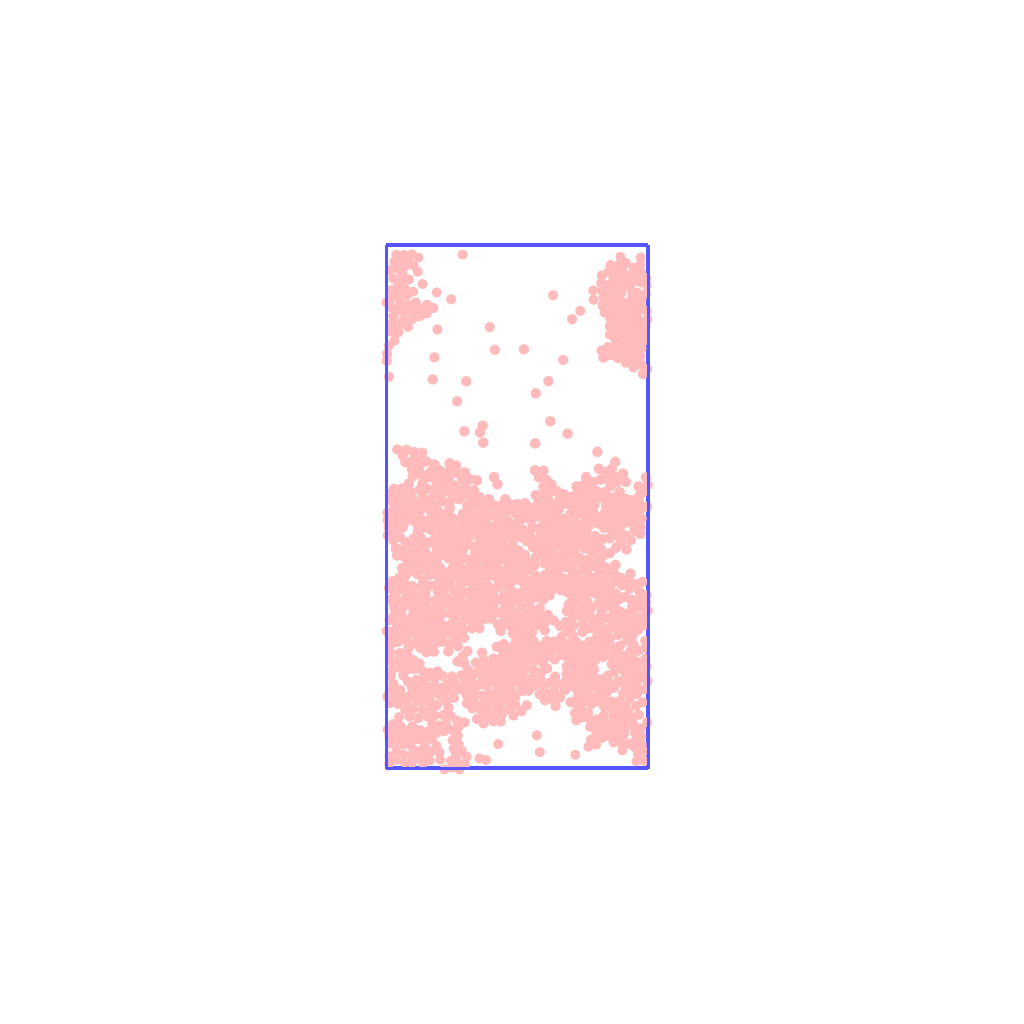
\includegraphics[width=\textwidth]{image/RaRtmap/2023-11-14T18:19:29.358__chi1.265_Ay50_rho0.4_T0.43_dT0.04_Rd0.0_Rt0.0_Ra0.0_g0.0003999718779659611_run4.0e7_output.png}}
      \subcaption{$\text{R}_\text{a}=0.0,\\\text{R}_\text{t}=0.0$}
      % \label{}
    \end{minipage} &
    \begin{minipage}[t]{0.2\hsize}
      \centering
      \href{https://youtu.be/4rNNLx9_DZ4}{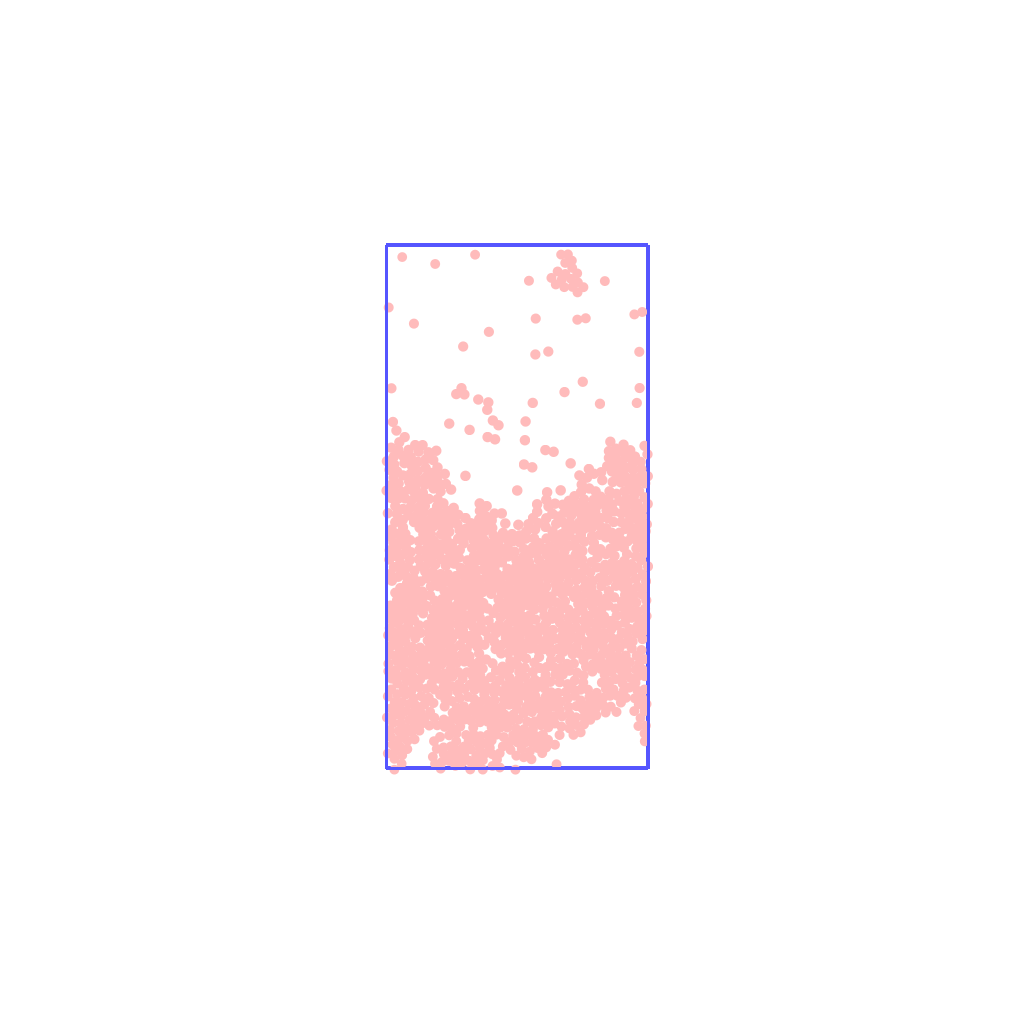
\includegraphics[width=\textwidth]{image/RaRtmap/2023-11-14T19:14:52.710__chi1.265_Ay50_rho0.4_T0.43_dT0.04_Rd0.0_Rt0.0_Ra0.4693845_g0.0003999718779659611_run4.0e7_output.png}}
      \subcaption{$\text{R}_\text{a}=0.469,\\\text{R}_\text{t}=0.0$}
      % \label{}
    \end{minipage} &
    \begin{minipage}[t]{0.2\hsize}
      \centering
      \href{https://youtu.be/QKLz7NzBte8}{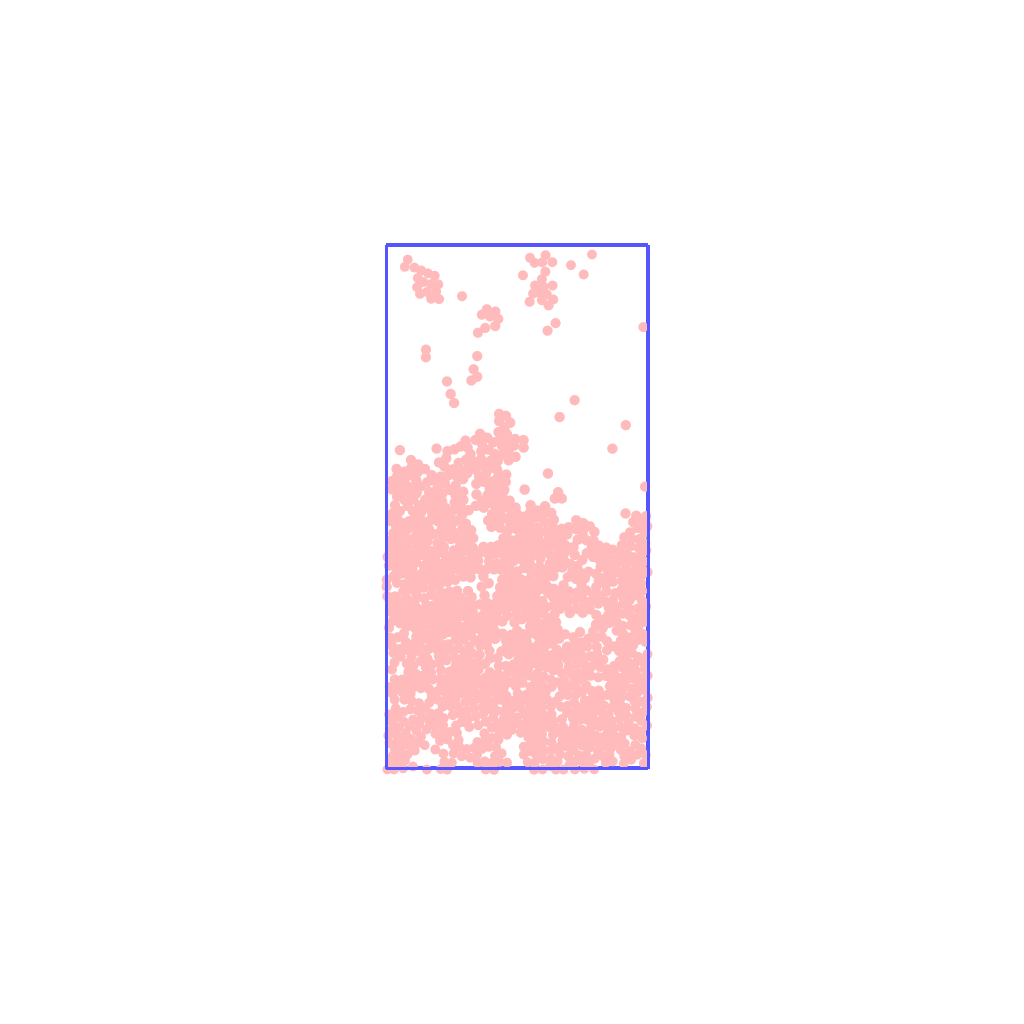
\includegraphics[width=\textwidth]{image/RaRtmap/2023-11-14T20:07:58.625__chi1.265_Ay50_rho0.4_T0.43_dT0.04_Rd0.0_Rt0.0_Ra0.938769_g0.0003999718779659611_run4.0e7_output.png}}
      \subcaption{$\text{R}_\text{a}=0.938,\\\text{R}_\text{t}=0.0$}
      % \label{}
    \end{minipage} &
    \begin{minipage}[t]{0.2\hsize}
      \centering
      \href{https://youtu.be/6iqcv_Af2U8}{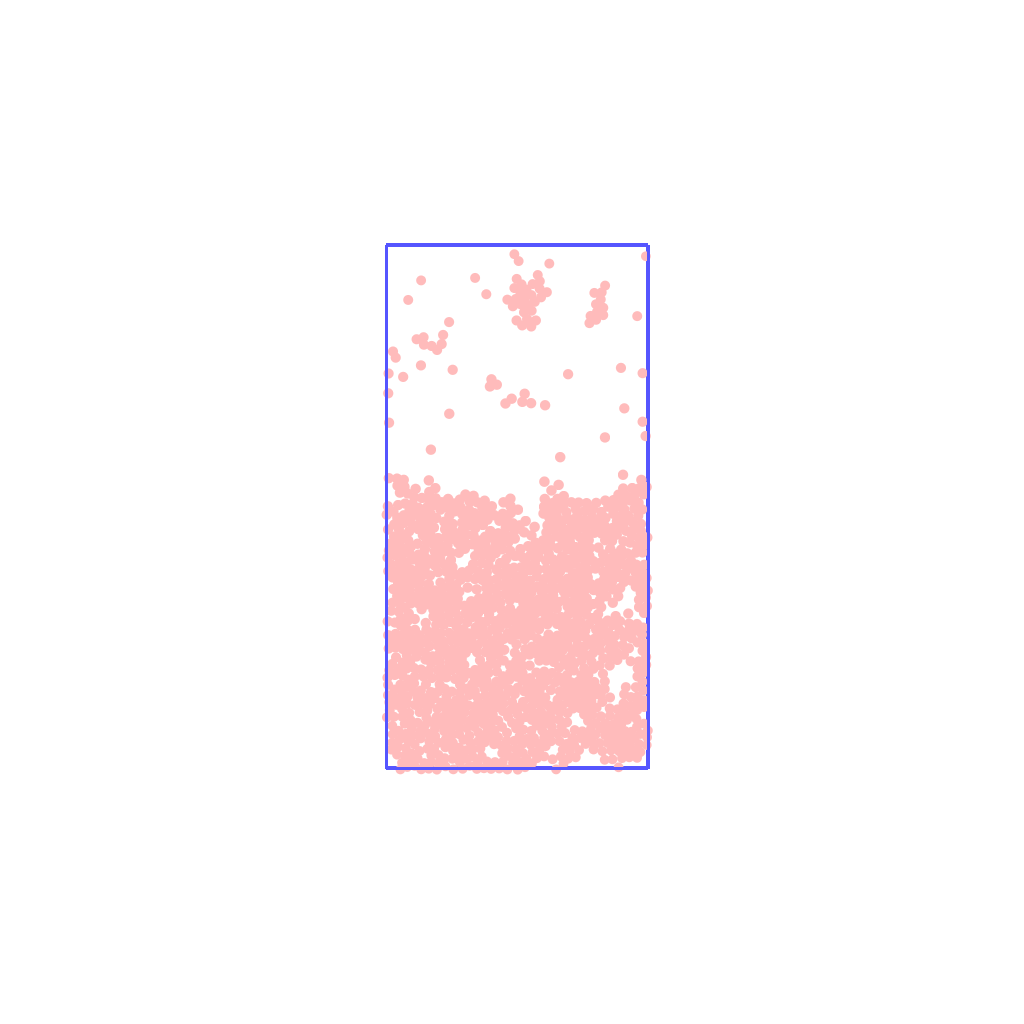
\includegraphics[width=\textwidth]{image/RaRtmap/2023-11-14T21:01:09.992__chi1.265_Ay50_rho0.4_T0.43_dT0.04_Rd0.0_Rt0.0_Ra1.4081535_g0.0003999718779659611_run4.0e7_output.png}}
      \subcaption{$\text{R}_\text{a}=1.408,\\\text{R}_\text{t}=0.0$}
      % \label{}
    \end{minipage} &
    \begin{minipage}[t]{0.2\hsize}
      \centering
      \href{https://youtu.be/Tn1Hd2eR0yo}{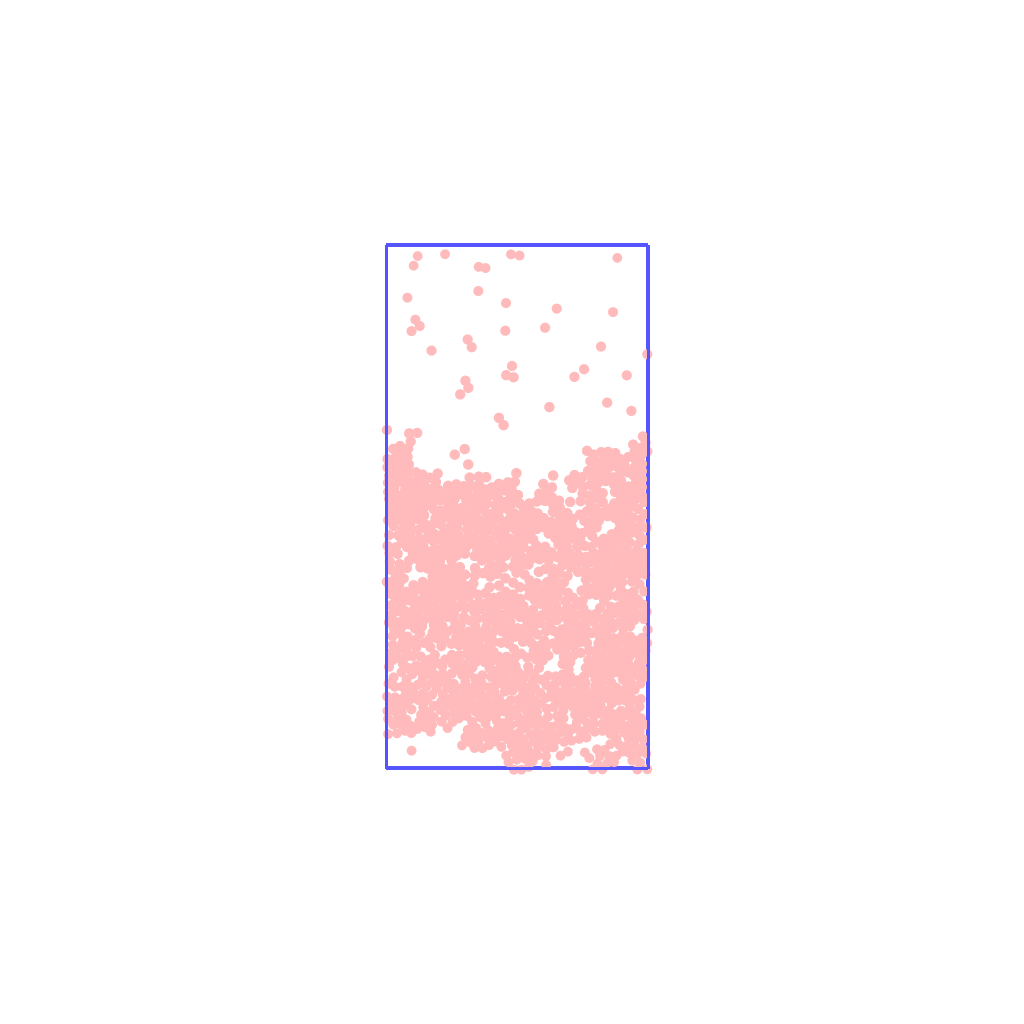
\includegraphics[width=\textwidth]{image/RaRtmap/2023-11-14T21:54:59.835__chi1.265_Ay50_rho0.4_T0.43_dT0.04_Rd0.0_Rt0.0_Ra1.877538_g0.0003999718779659611_run4.0e7_output.png}}
      \subcaption{$\text{R}_\text{a}=1.877,\\\text{R}_\text{t}=0.0$}
      % \label{}
    \end{minipage} \\
    \begin{minipage}[t]{0.2\hsize}
      \centering
      \href{https://youtu.be/B1GwQFCBszs}{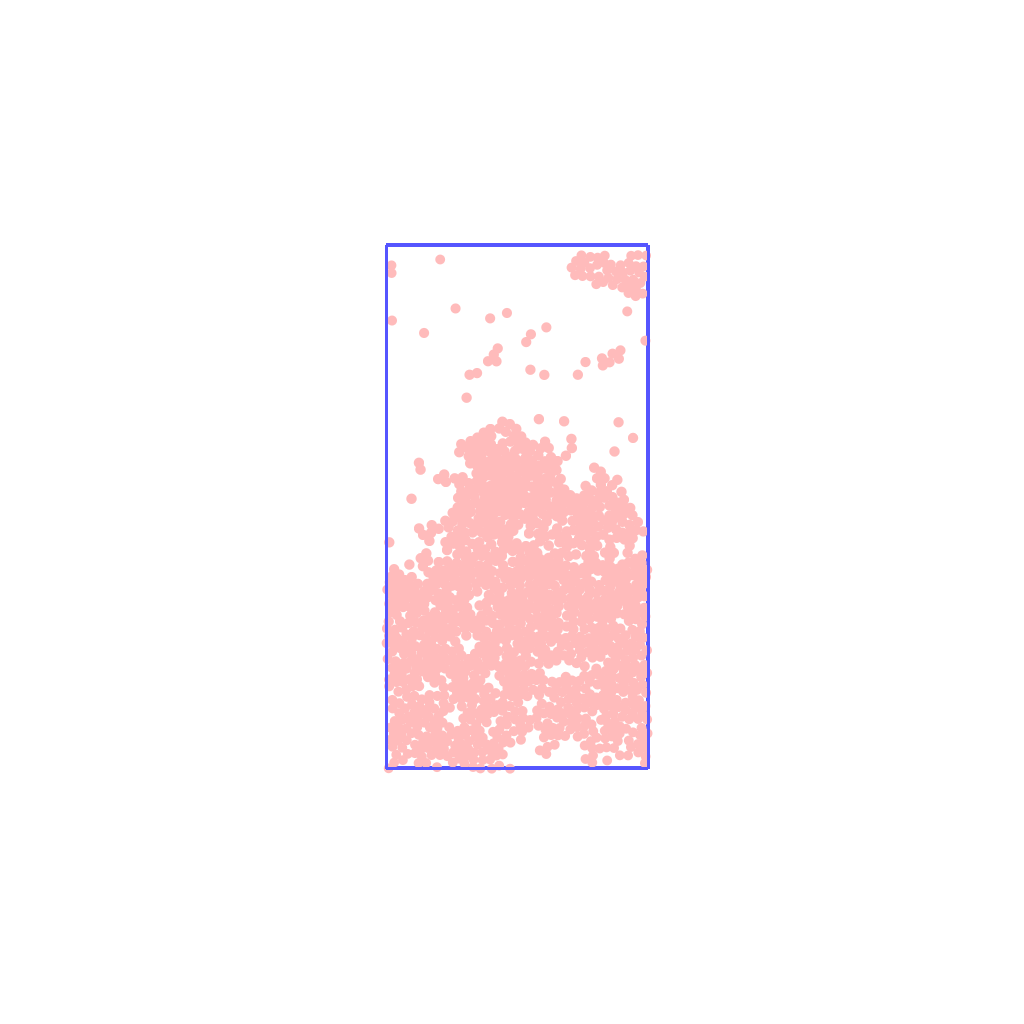
\includegraphics[width=\textwidth]{image/RaRtmap/2023-11-14T22:51:24.191__chi1.265_Ay50_rho0.4_T0.43_dT0.04_Rd0.0_Rt0.125_Ra0.0_g0.0003999718779659611_run4.0e7_output.png}}
      \subcaption{$\text{R}_\text{a}=0.0,\\\text{R}_\text{t}=0.125$}
      % \label{}
    \end{minipage} &
    \begin{minipage}[t]{0.2\hsize}
      \centering
      \href{https://youtu.be/MRIfAketXOI}{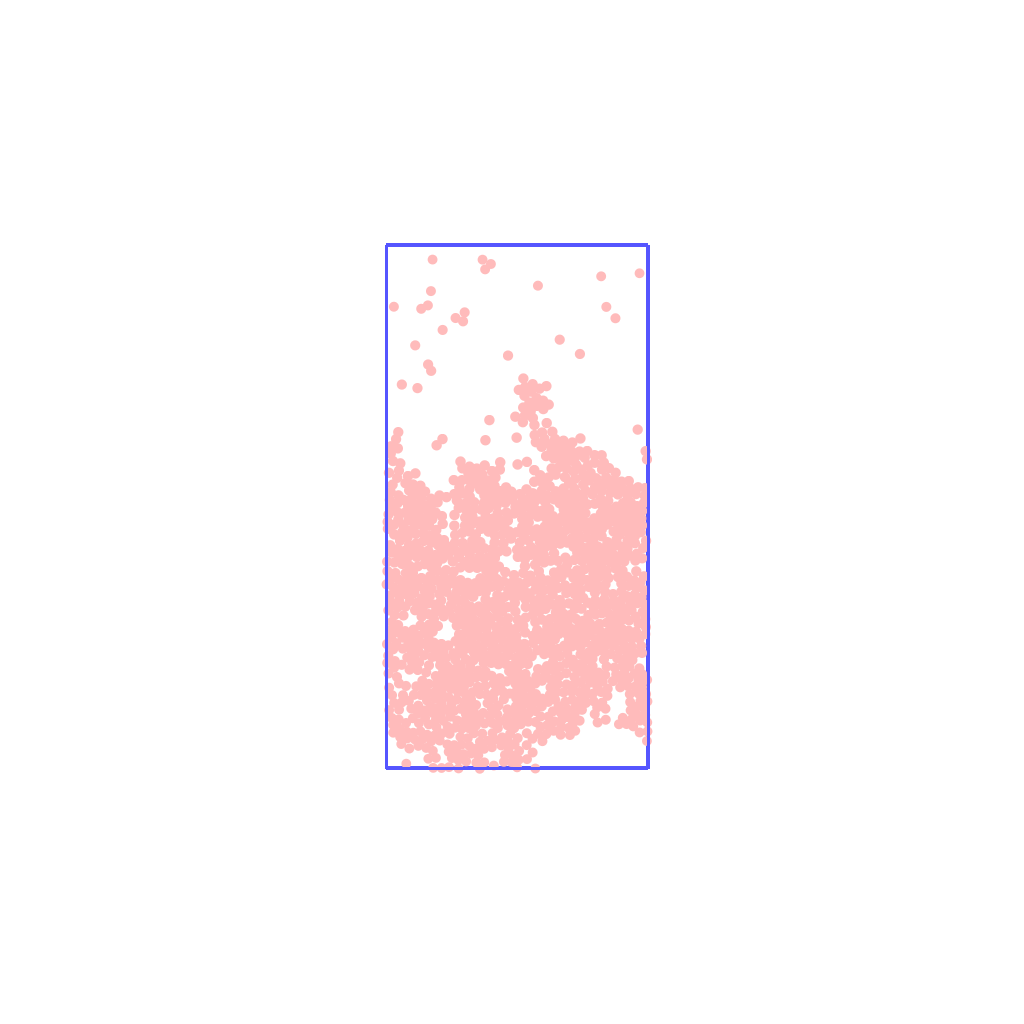
\includegraphics[width=\textwidth]{image/RaRtmap/2023-11-14T23:48:31.439__chi1.265_Ay50_rho0.4_T0.43_dT0.04_Rd0.0_Rt0.125_Ra0.4693845_g0.0003999718779659611_run4.0e7_output.png}}
      \subcaption{$\text{R}_\text{a}=0.469,\\\text{R}_\text{t}=0.125$}
      % \label{}
    \end{minipage} &
    \begin{minipage}[t]{0.2\hsize}
      \centering
      \href{https://youtu.be/v7rYxdoSSjI}{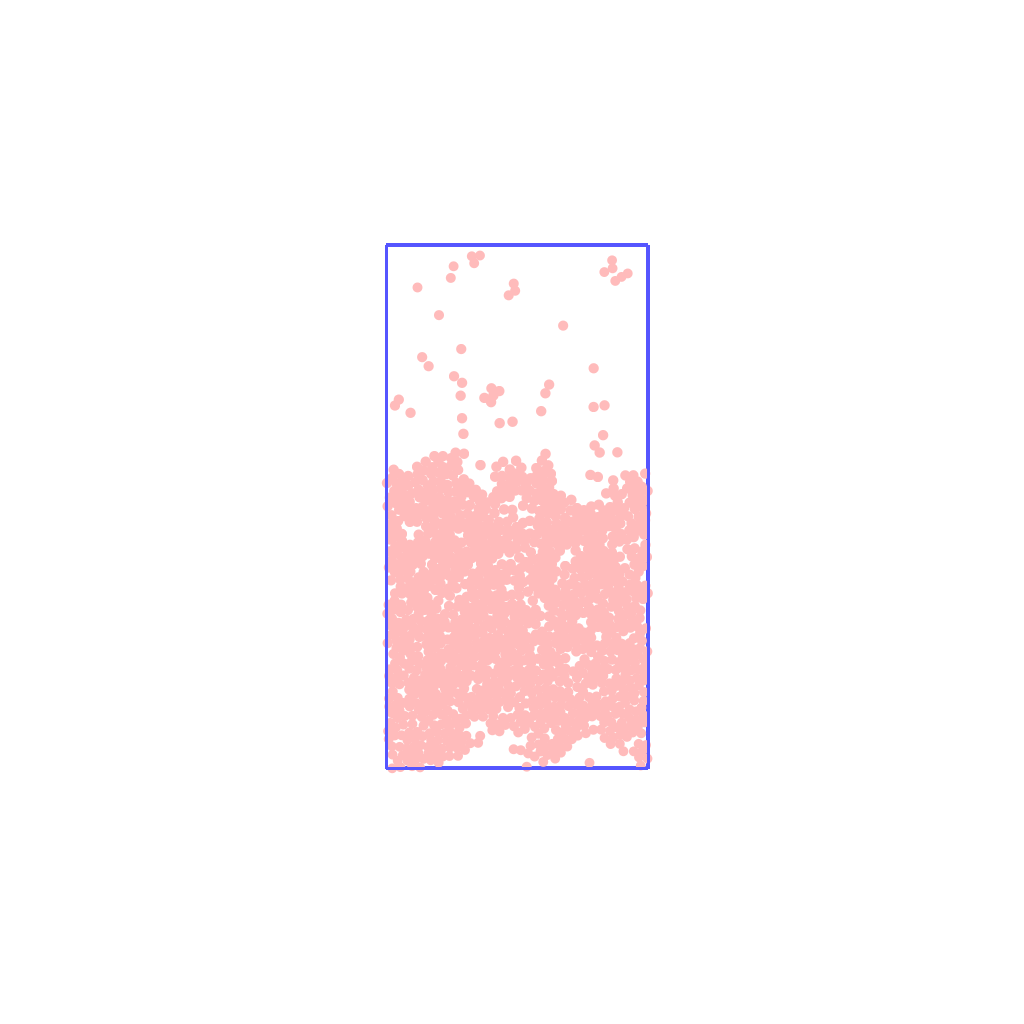
\includegraphics[width=\textwidth]{image/RaRtmap/2023-11-15T00:43:33.781__chi1.265_Ay50_rho0.4_T0.43_dT0.04_Rd0.0_Rt0.125_Ra0.938769_g0.0003999718779659611_run4.0e7_output.png}}
      \subcaption{$\text{R}_\text{a}=0.938,\\\text{R}_\text{t}=0.125$}
      % \label{}
    \end{minipage} &
    \begin{minipage}[t]{0.2\hsize}
      \centering
      \href{https://youtu.be/0NFYPFYBcc4}{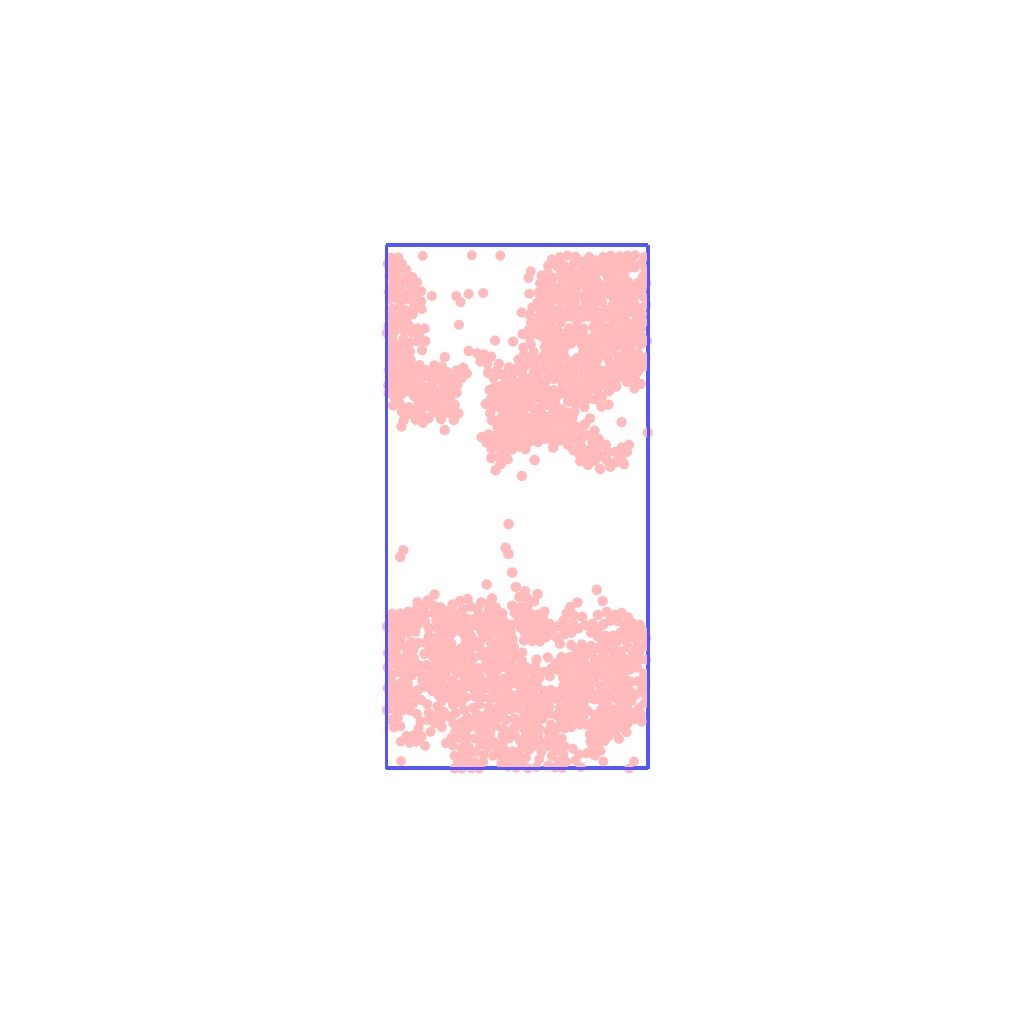
\includegraphics[width=\textwidth]{image/RaRtmap/2023-11-15T01:35:17.404__chi1.265_Ay50_rho0.4_T0.43_dT0.04_Rd0.0_Rt0.125_Ra1.4081535_g0.0003999718779659611_run4.0e7_output.png}}
      \subcaption{$\text{R}_\text{a}=1.408,\\\text{R}_\text{t}=0.125$}
      % \label{}
    \end{minipage} &
    \begin{minipage}[t]{0.2\hsize}
      \centering
      \href{https://youtu.be/FXTDOcpARl0}{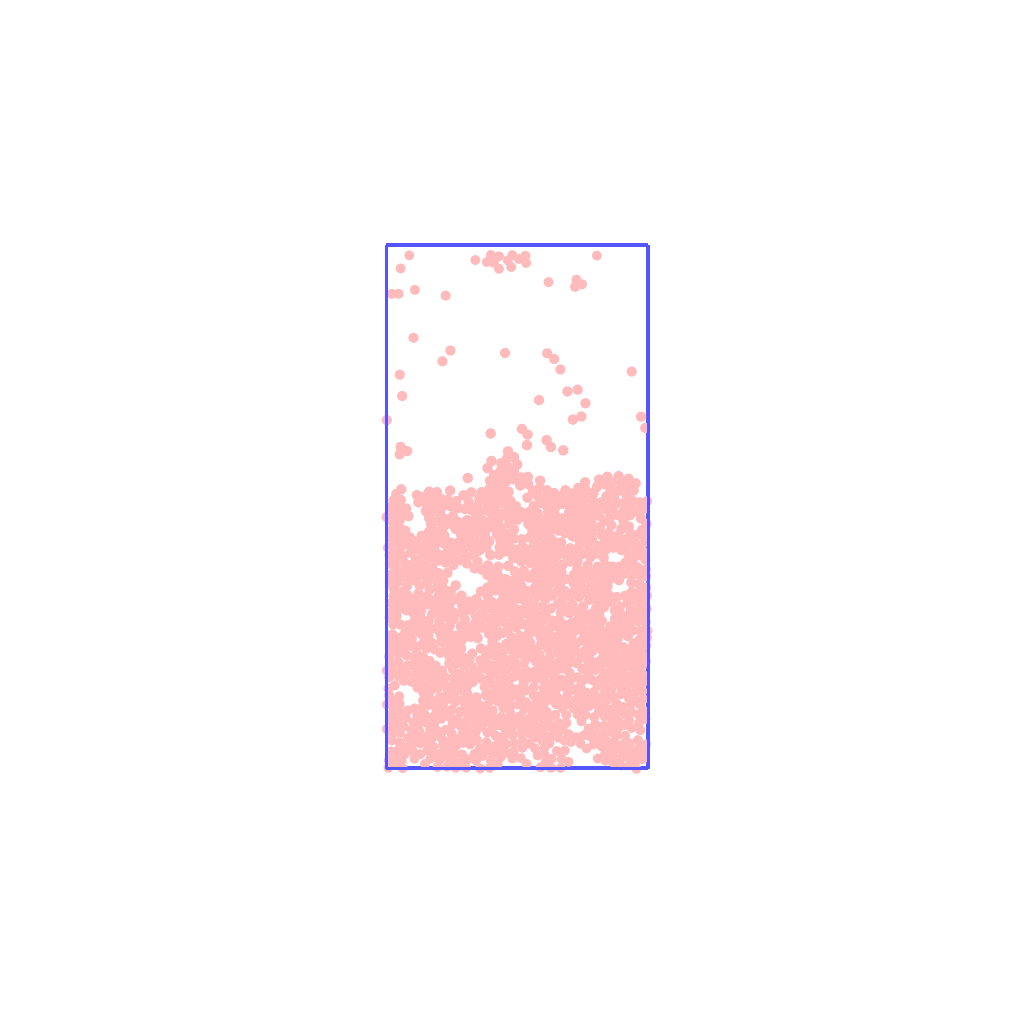
\includegraphics[width=\textwidth]{image/RaRtmap/2023-11-15T02:27:34.337__chi1.265_Ay50_rho0.4_T0.43_dT0.04_Rd0.0_Rt0.125_Ra1.877538_g0.0003999718779659611_run4.0e7_output.png}}
      \subcaption{$\text{R}_\text{a}=1.877,\\\text{R}_\text{t}=0.125$}
      % \label{}
    \end{minipage} \\
    \begin{minipage}[t]{0.2\hsize}
      \centering
      \href{https://youtu.be/4A\_MHNHZrKQ}{
      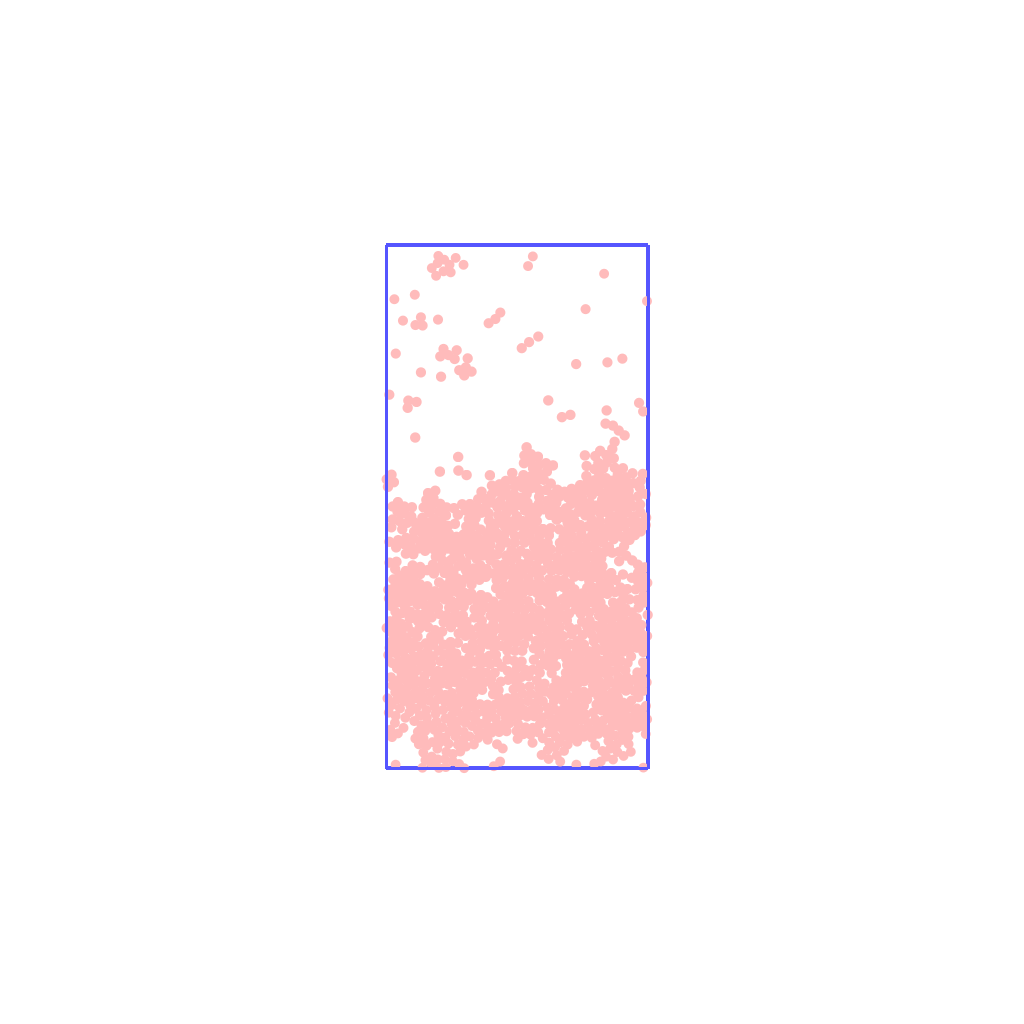
\includegraphics[width=\textwidth]{image/RaRtmap/2023-11-15T03:19:32.715__chi1.265_Ay50_rho0.4_T0.43_dT0.04_Rd0.0_Rt0.25_Ra0.0_g0.0003999718779659611_run4.0e7_output.png}}
      \subcaption{$\text{R}_\text{a}=0.0,\\\text{R}_\text{t}=0.250$}
      % \label{}
    \end{minipage} &
    \begin{minipage}[t]{0.2\hsize}
      \centering
      \href{https://youtu.be/jGzUPm\_3oH0}{
      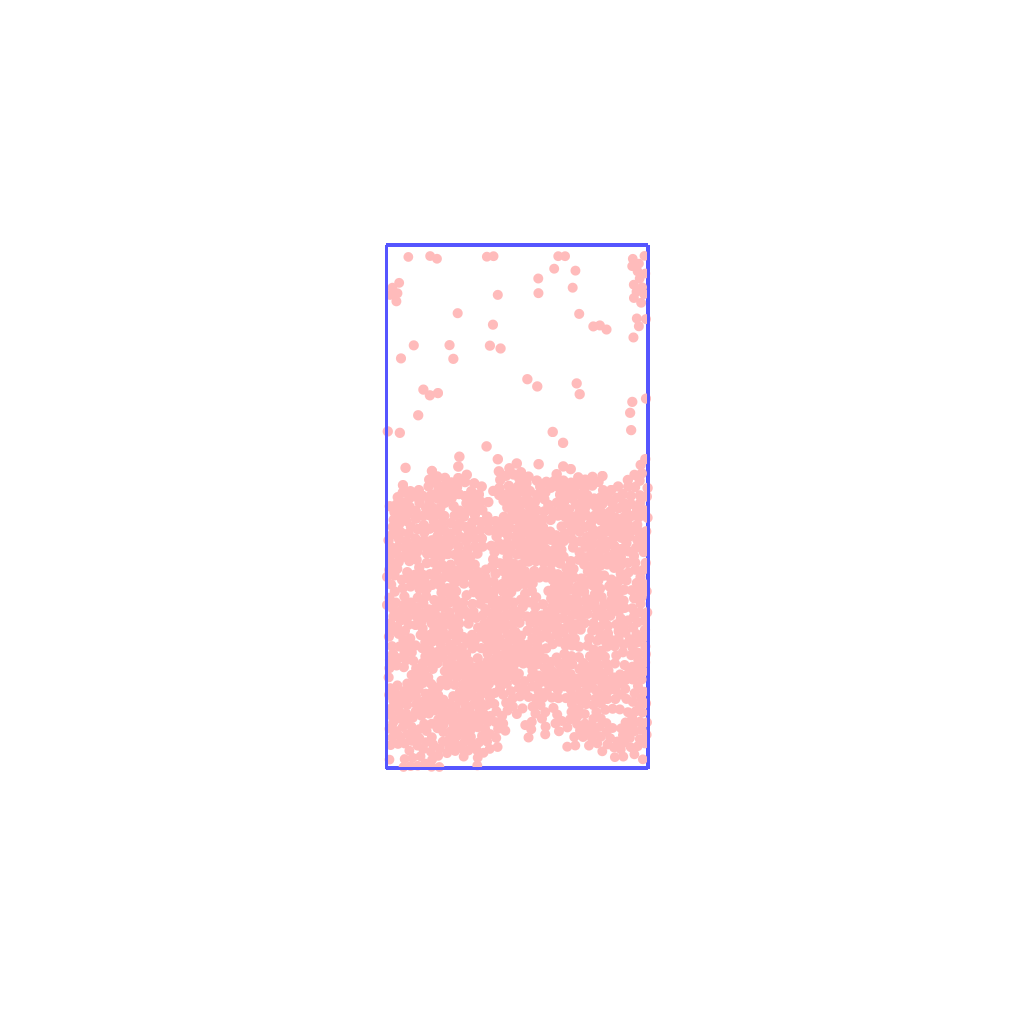
\includegraphics[width=\textwidth]{image/RaRtmap/2023-11-15T04:11:00.956__chi1.265_Ay50_rho0.4_T0.43_dT0.04_Rd0.0_Rt0.25_Ra0.4693845_g0.0003999718779659611_run4.0e7_output.png}}
      \subcaption{$\text{R}_\text{a}=0.469,\\\text{R}_\text{t}=0.250$}
      % \label{}
    \end{minipage} &
    \begin{minipage}[t]{0.2\hsize}
      \centering
      \href{https://youtu.be/0iyDEBwDF7A}{
      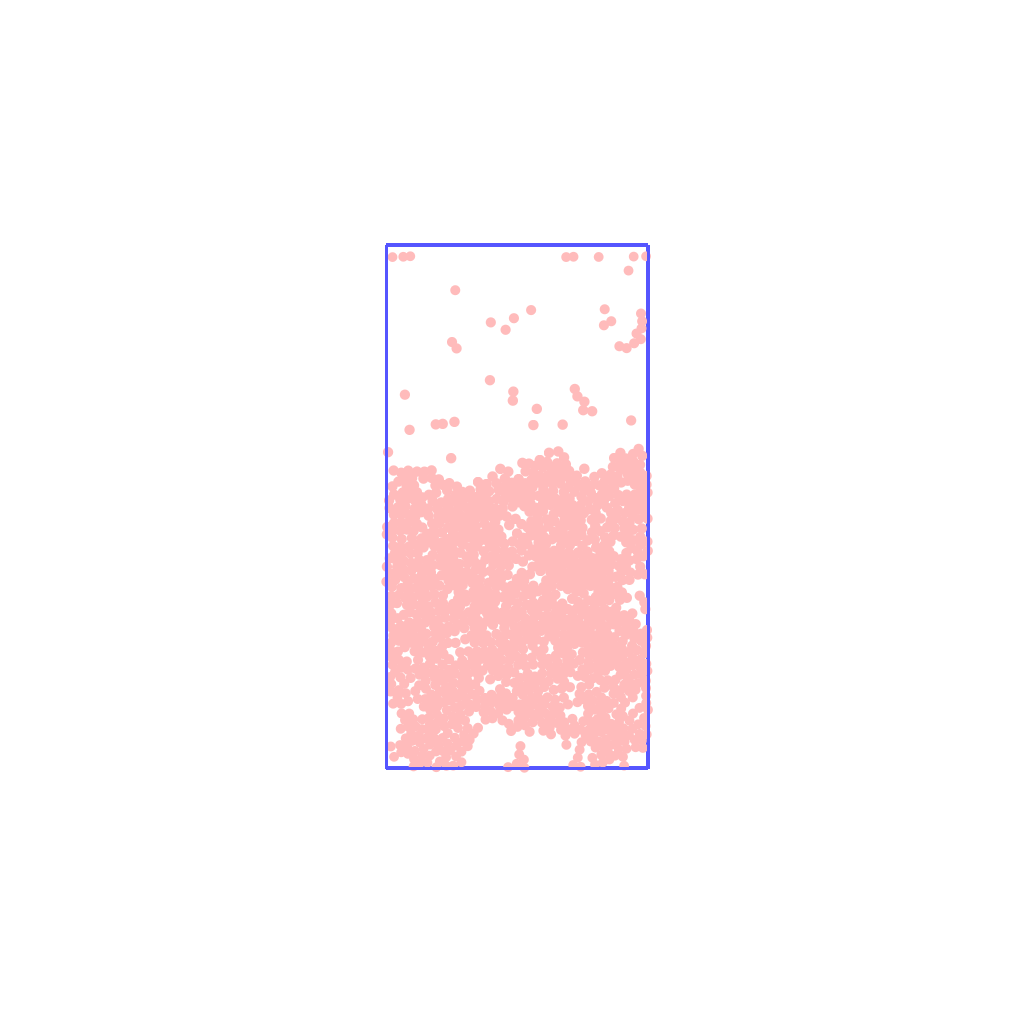
\includegraphics[width=\textwidth]{image/RaRtmap/2023-11-15T05:03:45.973__chi1.265_Ay50_rho0.4_T0.43_dT0.04_Rd0.0_Rt0.25_Ra0.938769_g0.0003999718779659611_run4.0e7_output.png}}
      \subcaption{$\text{R}_\text{a}=0.938,\\\text{R}_\text{t}=0.250$}
      % \label{}
    \end{minipage} &
    \begin{minipage}[t]{0.2\hsize}
      \centering
      \href{https://youtu.be/Sqk3HDSDINw}{
      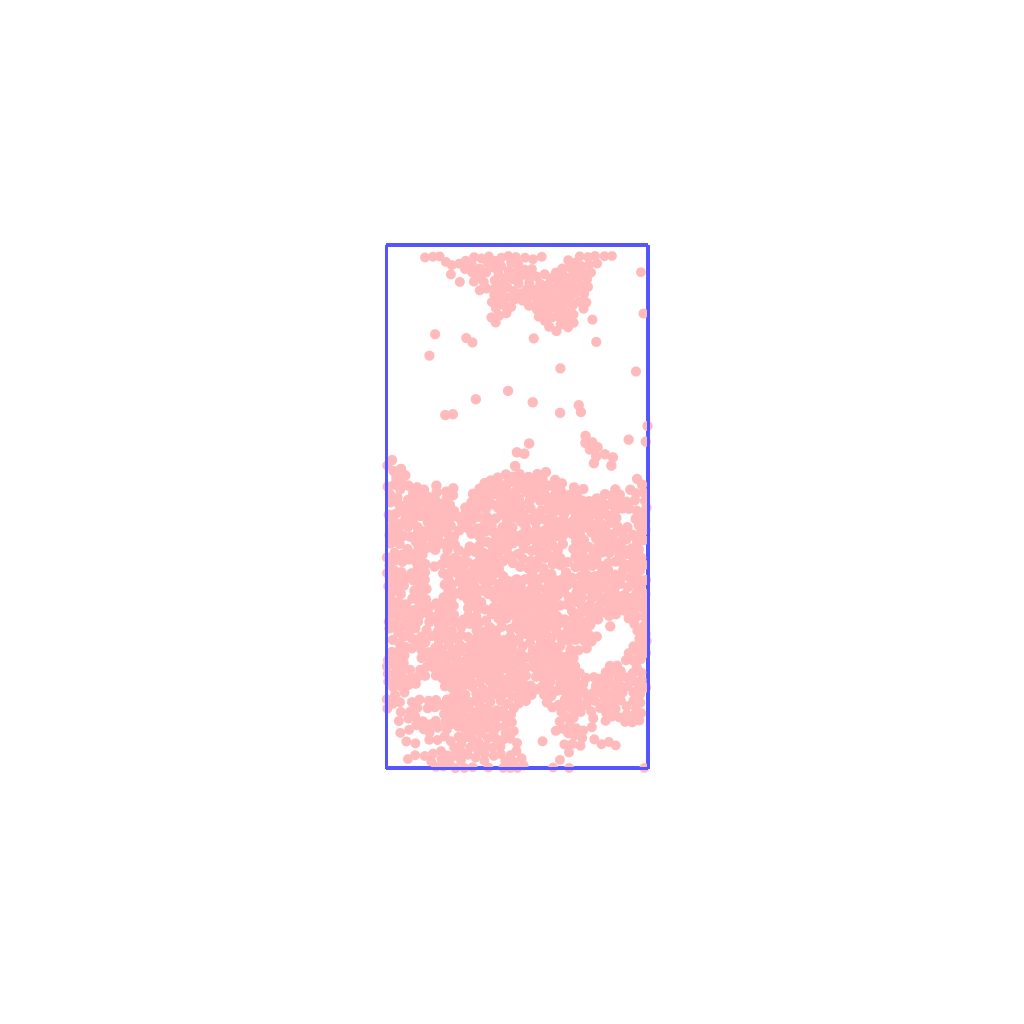
\includegraphics[width=\textwidth]{image/RaRtmap/2023-11-15T05:53:00.667__chi1.265_Ay50_rho0.4_T0.43_dT0.04_Rd0.0_Rt0.25_Ra1.4081535_g0.0003999718779659611_run4.0e7_output.png}}
      \subcaption{$\text{R}_\text{a}=1.408,\\\text{R}_\text{t}=0.250$}
      % \label{}
    \end{minipage} &
    \begin{minipage}[t]{0.2\hsize}
      \centering
      \href{https://youtu.be/3lqCLQchVYA}{
      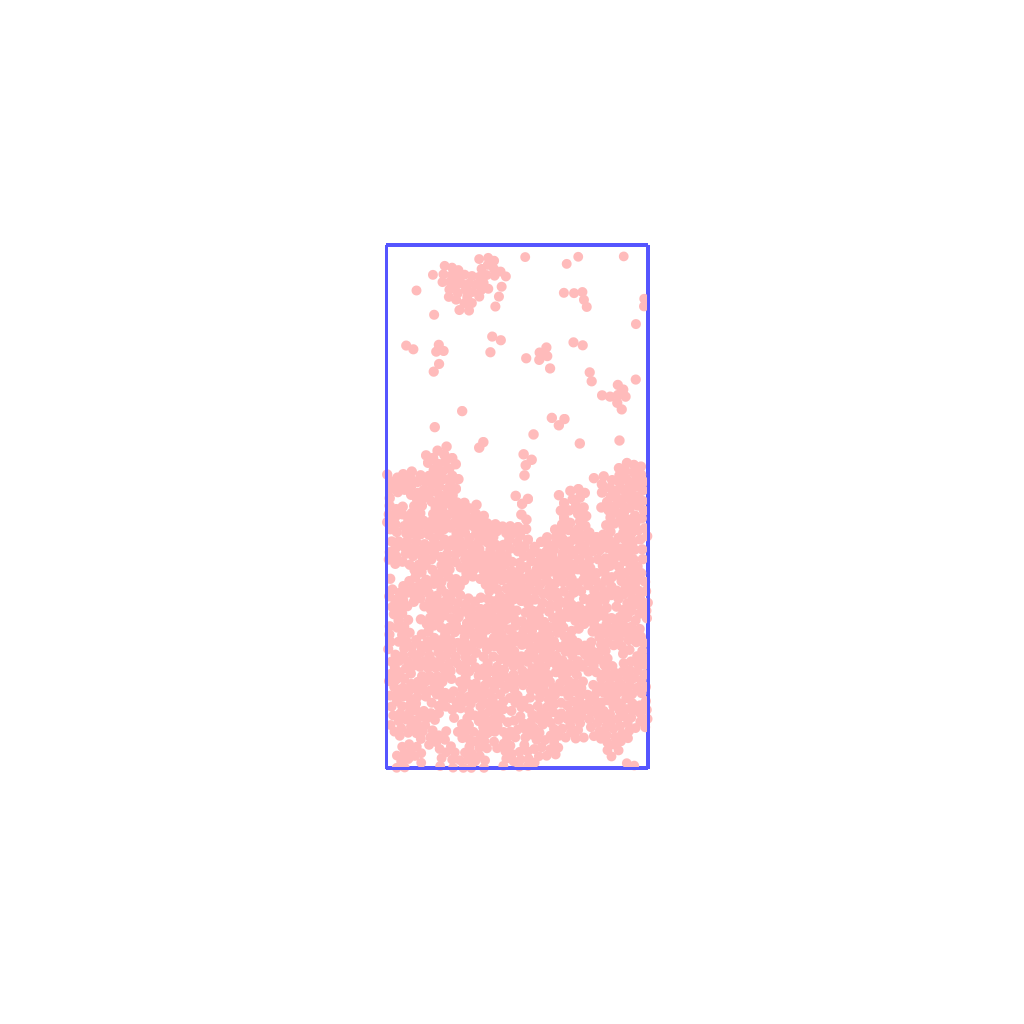
\includegraphics[width=\textwidth]{image/RaRtmap/2023-11-15T06:43:21.554__chi1.265_Ay50_rho0.4_T0.43_dT0.04_Rd0.0_Rt0.25_Ra1.877538_g0.0003999718779659611_run4.0e7_output.png}}
      \subcaption{$\text{R}_\text{a}=1.877,\\\text{R}_\text{t}=0.250$}
      % \label{}
    \end{minipage} \\
    \begin{minipage}[t]{0.2\hsize}
      \centering
      \href{https://youtu.be/1cMmZVmcThA}{
      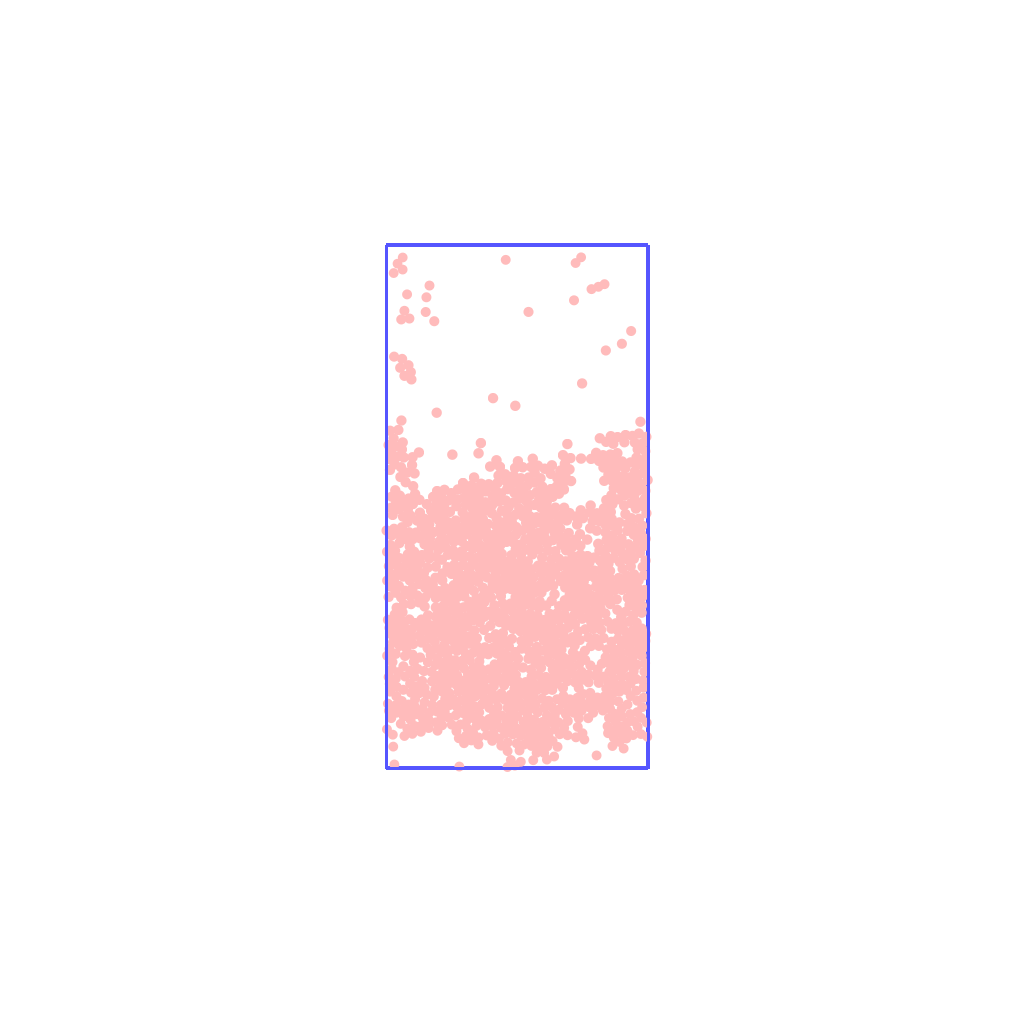
\includegraphics[width=\textwidth]{image/RaRtmap/2023-11-15T07:34:00.555__chi1.265_Ay50_rho0.4_T0.43_dT0.04_Rd0.0_Rt0.375_Ra0.0_g0.0003999718779659611_run4.0e7_output.png}}
      \subcaption{$\text{R}_\text{a}=0.0,\\\text{R}_\text{t}=0.375$}
      % \label{}
    \end{minipage} &
    \begin{minipage}[t]{0.2\hsize}
      \centering
      \href{https://youtu.be/MDWWS7Axo-4}{
      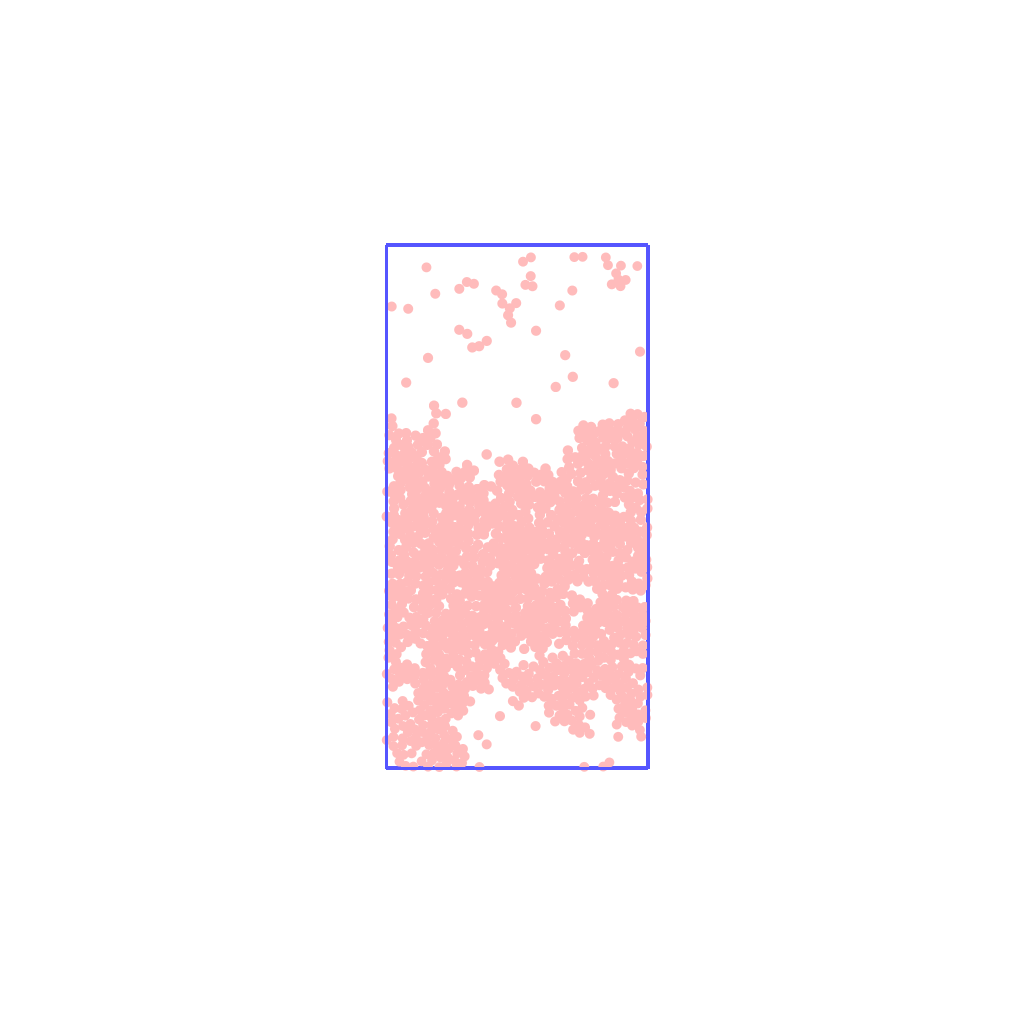
\includegraphics[width=\textwidth]{image/RaRtmap/2023-11-15T08:24:37.362__chi1.265_Ay50_rho0.4_T0.43_dT0.04_Rd0.0_Rt0.375_Ra0.4693845_g0.0003999718779659611_run4.0e7_output.png}}
      \subcaption{$\text{R}_\text{a}=0.469,\\\text{R}_\text{t}=0.375$}
      % \label{}
    \end{minipage} &
    \begin{minipage}[t]{0.2\hsize}
      \centering
      \href{https://youtu.be/Y6O_tVs6mHY}{
      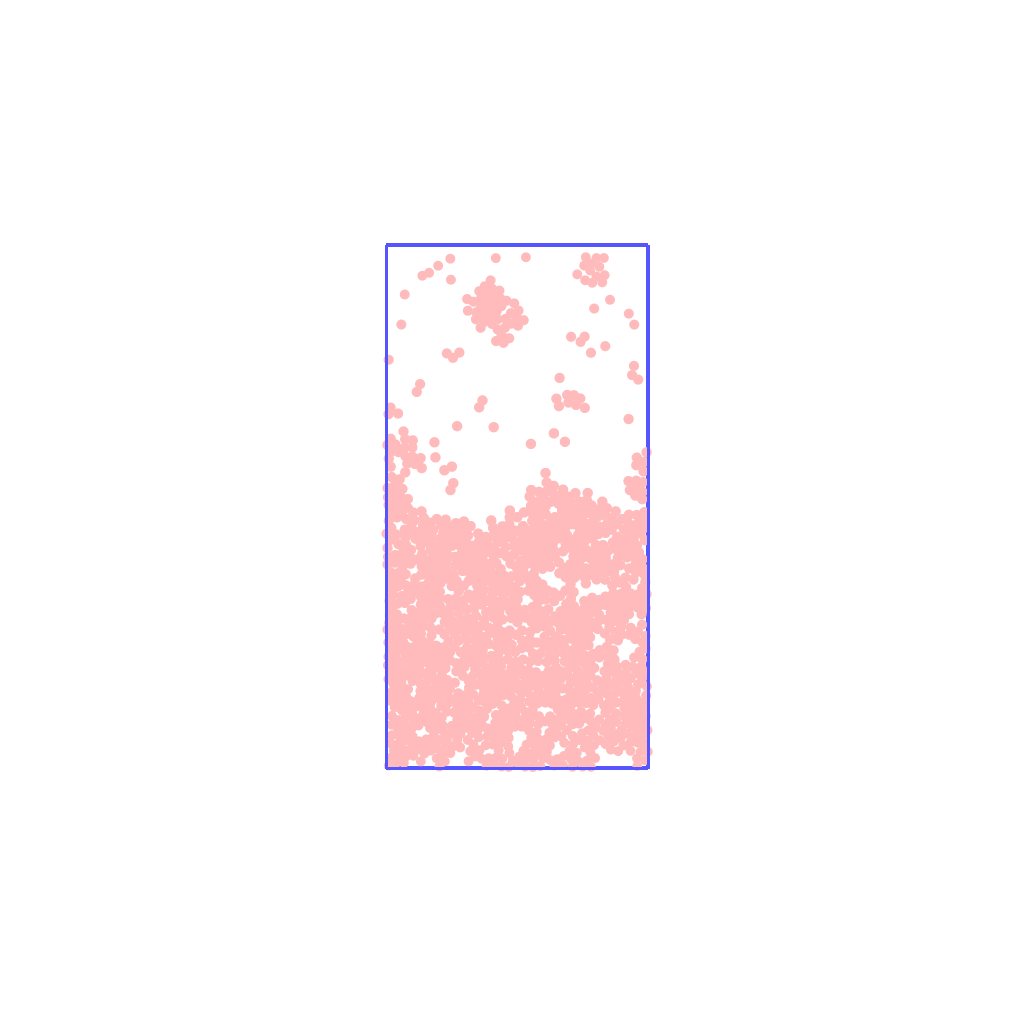
\includegraphics[width=\textwidth]{image/RaRtmap/2023-11-15T09:16:40.082__chi1.265_Ay50_rho0.4_T0.43_dT0.04_Rd0.0_Rt0.375_Ra0.938769_g0.0003999718779659611_run4.0e7_output.png}}
      \subcaption{$\text{R}_\text{a}=0.938,\\\text{R}_\text{t}=0.375$}
      % \label{}
    \end{minipage} &
    \begin{minipage}[t]{0.2\hsize}
      \centering
      \href{https://youtu.be/yeI5CDT0TEw}{
      
\includegraphics[width=\textwidth]{image/RaRtmap/2023-11-15T10:07:20.945__chi1.265_Ay50_rho0.4_T0.43_dT0.04_Rd0.0_Rt0.375_Ra1.4081535_g0.0003999718779659611_run4.0e7_output.png}}
      \subcaption{$\text{R}_\text{a}=1.408,\\\text{R}_\text{t}=0.375$}
      % \label{}
    \end{minipage} &
    \begin{minipage}[t]{0.2\hsize}
      \centering
      \href{https://youtu.be/h6w-DYqP-bg}{
      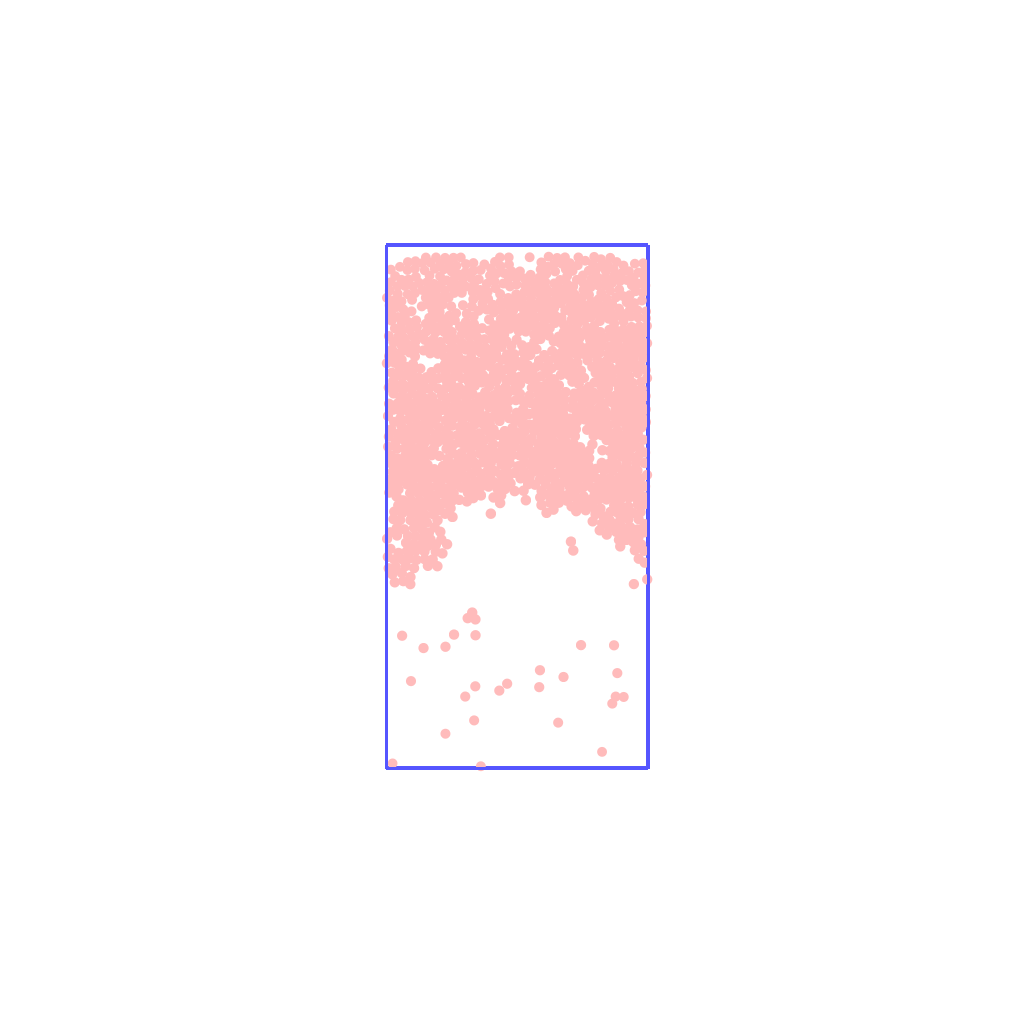
\includegraphics[width=\textwidth]{image/RaRtmap/2023-11-15T10:59:30.665__chi1.265_Ay50_rho0.4_T0.43_dT0.04_Rd0.0_Rt0.375_Ra1.877538_g0.0003999718779659611_run4.0e7_output.png}}
      \subcaption{$\text{R}_\text{a}=1.877,\\\text{R}_\text{t}=0.375$}
      % \label{}
    \end{minipage} \\
    \begin{minipage}[t]{0.2\hsize}
      \centering
      \href{https://youtu.be/S0NOYiYNCBU}{
      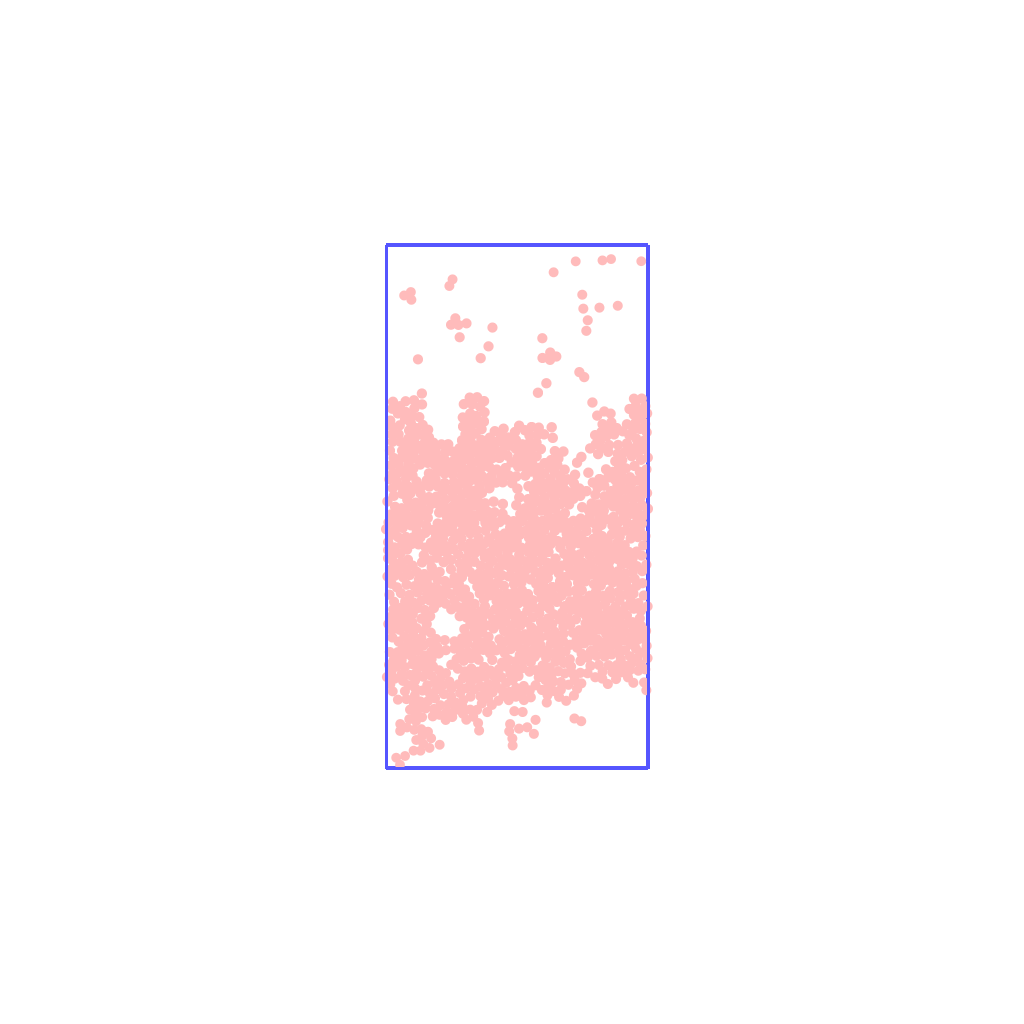
\includegraphics[width=\textwidth]{image/RaRtmap/2023-11-15T11:53:37.697__chi1.265_Ay50_rho0.4_T0.43_dT0.04_Rd0.0_Rt0.5_Ra0.0_g0.0003999718779659611_run4.0e7_output.png}}
      \subcaption{$\text{R}_\text{a}=0.0,\\\text{R}_\text{t}=0.500$}
      % \label{}
    \end{minipage} &
    \begin{minipage}[t]{0.2\hsize}
      \centering
      \href{https://youtu.be/l8Mz0kOFZwY}{
      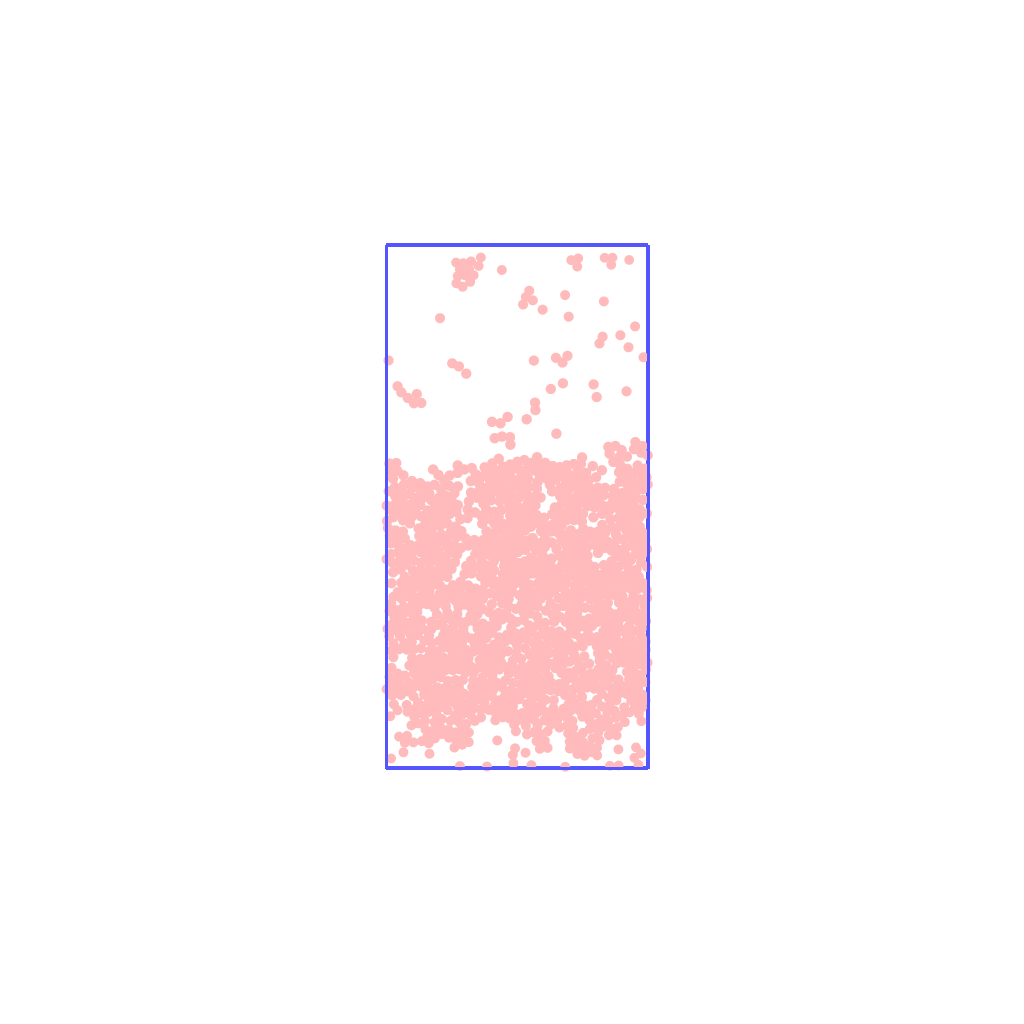
\includegraphics[width=\textwidth]{image/RaRtmap/2023-11-15T12:45:26.303__chi1.265_Ay50_rho0.4_T0.43_dT0.04_Rd0.0_Rt0.5_Ra0.4693845_g0.0003999718779659611_run4.0e7_output.png}}
      \subcaption{$\text{R}_\text{a}=0.469,\\\text{R}_\text{t}=0.500$}
      % \label{}
    \end{minipage} &
    \begin{minipage}[t]{0.2\hsize}
      \centering
      \href{https://youtu.be/pR-P4R70FQg}{
      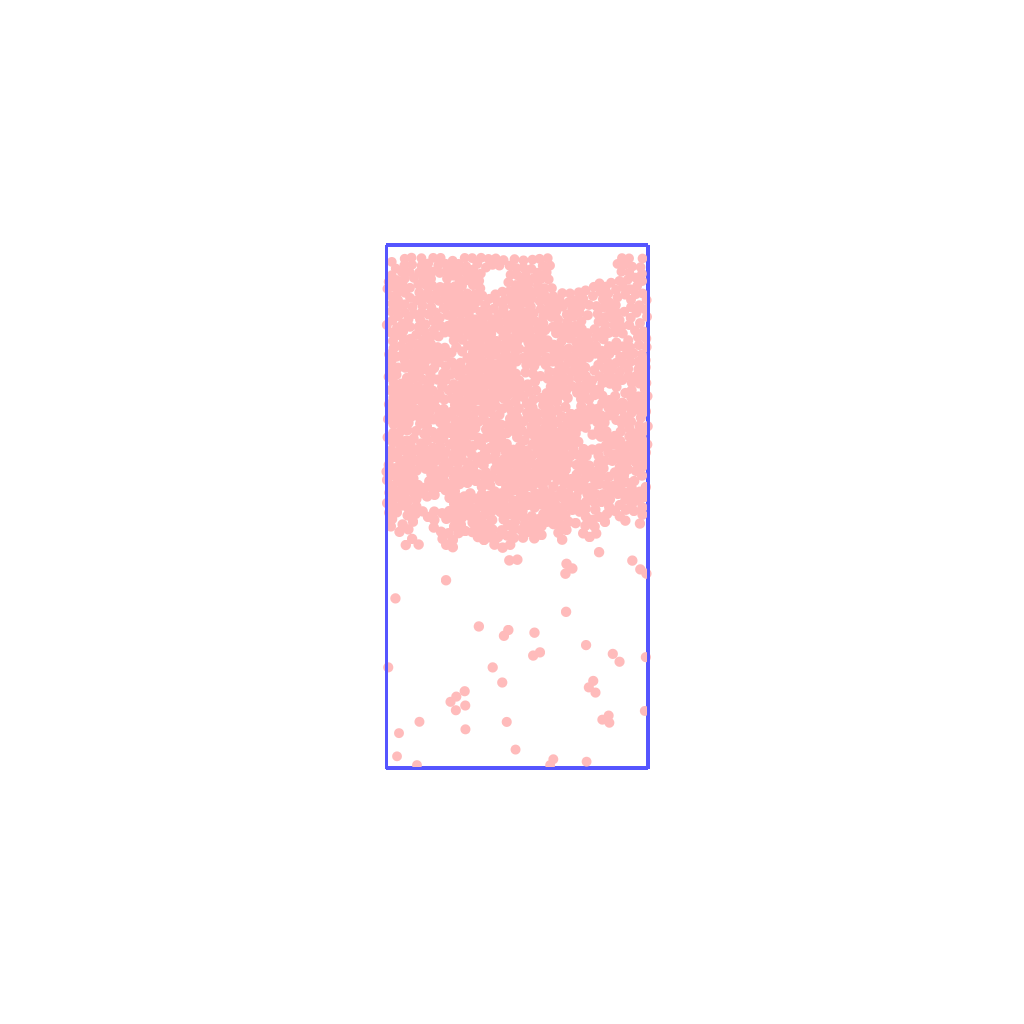
\includegraphics[width=\textwidth]{image/RaRtmap/2023-11-15T13:37:58.058__chi1.265_Ay50_rho0.4_T0.43_dT0.04_Rd0.0_Rt0.5_Ra0.938769_g0.0003999718779659611_run4.0e7_output.png}}
      \subcaption{$\text{R}_\text{a}=0.938,\\\text{R}_\text{t}=0.500$}
      % \label{}
    \end{minipage} &
    \begin{minipage}[t]{0.2\hsize}
      \centering
      \href{https://youtu.be/kSUk1XcKZBA}{
      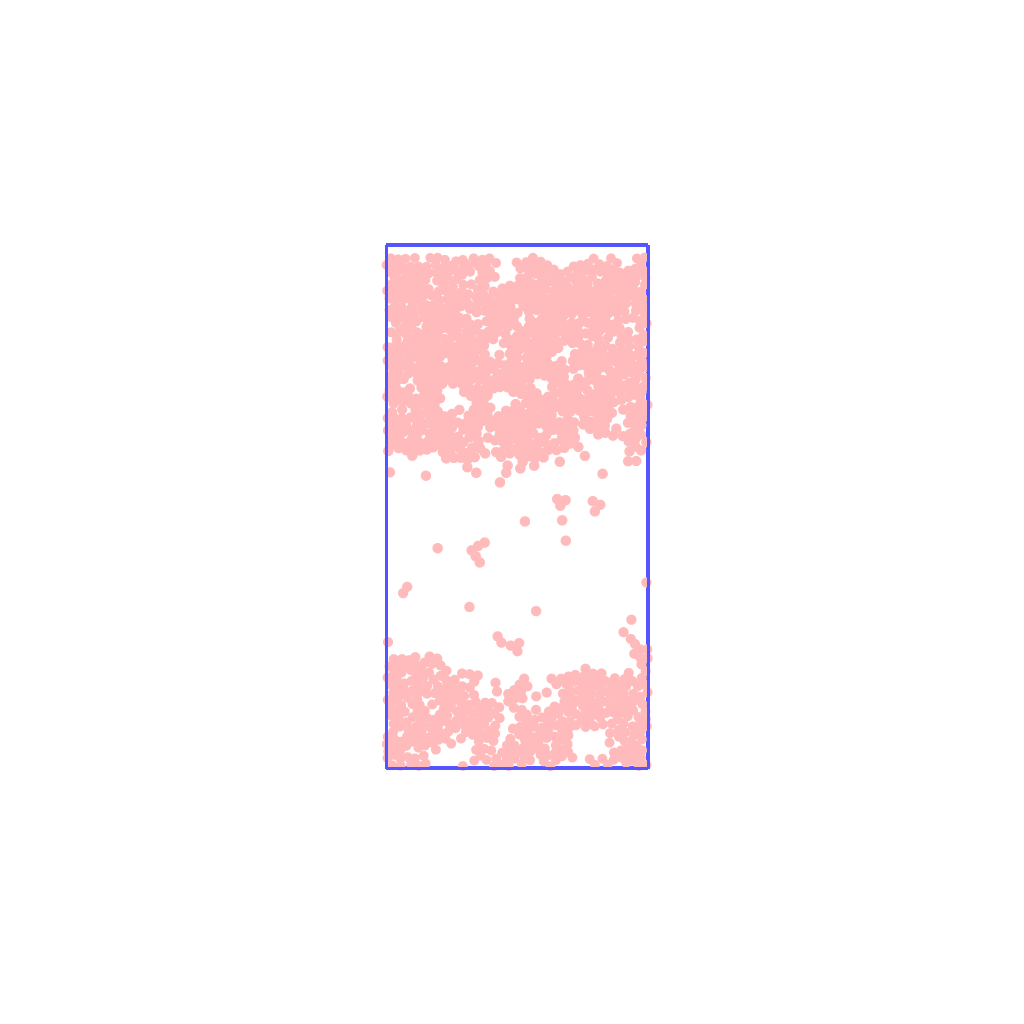
\includegraphics[width=\textwidth]{image/RaRtmap/2023-11-15T14:30:22.529__chi1.265_Ay50_rho0.4_T0.43_dT0.04_Rd0.0_Rt0.5_Ra1.4081535_g0.0003999718779659611_run4.0e7_output.png}}
      \subcaption{$\text{R}_\text{a}=1.408,\\\text{R}_\text{t}=0.500$}
      % \label{}
    \end{minipage} &
    \begin{minipage}[t]{0.2\hsize}
      \centering
      
\includegraphics[width=\textwidth]{image/RaRtmap/2023-11-15T15:21:59.073__chi1.265_Ay50_rho0.4_T0.43_dT0.04_Rd0.0_Rt0.5_Ra1.877538_g0.0003999718779659611_run4.0e7_output.png}
      \subcaption{$\text{R}_\text{a}=1.877,\\\text{R}_\text{t}=0.500$}
      % \label{}
    \end{minipage} 
  \end{tabular}
  \caption{}
  % \lable{}
\end{figure}


スナップショットだけではダイナミクスがわからないので, 次に図\ref{fig:RaRtmap_time}で重心位置$Y_g$(式\eqref{CoM})の時間変化の様子を見る. 

\begin{align}
  \label{CoM}
  Y_g &\equiv \bar{y_i} = \frac{1}{N} \sum_{i}^{N} y_i
\end{align}

重心位置$Y_g$を, 系の$y$幅を用いて$0\sim 1$にスケーリングして, 時系列プロットしている.

\begin{figure}[H]
  \begin{tabular}{ccccc}
    \begin{minipage}[t]{0.2\hsize}
      \centering
      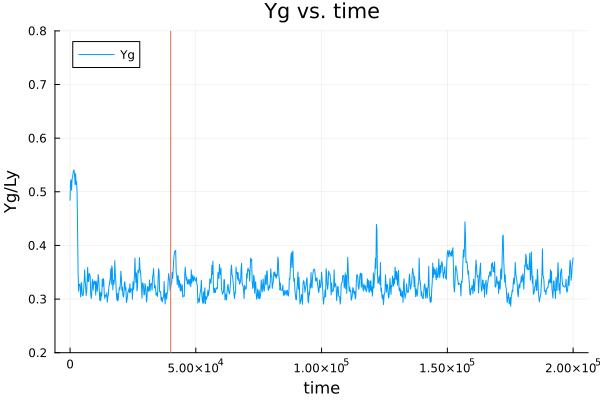
\includegraphics[width=\textwidth]{image/RaRtmap_time/2023-11-14T18:19:29.358__chi1.265_Ay50_rho0.4_T0.43_dT0.04_Rd0.0_Rt0.0_Ra0.0_g0.0003999718779659611_run4.0e7_output.png}
      \subcaption{$\text{R}_\text{a}=0.0,\\\text{R}_\text{t}=0.0$}
      \label{fig:RaRtmap_time_Ra0.0_Rt0.0}
    \end{minipage} &
    \begin{minipage}[t]{0.2\hsize}
      \centering
      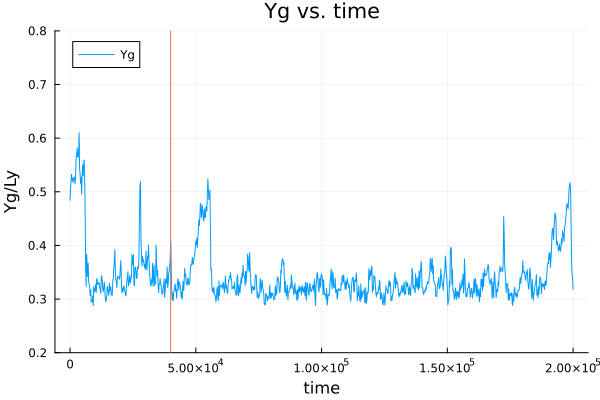
\includegraphics[width=\textwidth]{image/RaRtmap_time/2023-11-14T19:14:52.710__chi1.265_Ay50_rho0.4_T0.43_dT0.04_Rd0.0_Rt0.0_Ra0.4693845_g0.0003999718779659611_run4.0e7_output.png}
      \subcaption{$\text{R}_\text{a}=0.469,\\\text{R}_\text{t}=0.0$}
      \label{}
    \end{minipage} &
    \begin{minipage}[t]{0.2\hsize}
      \centering
      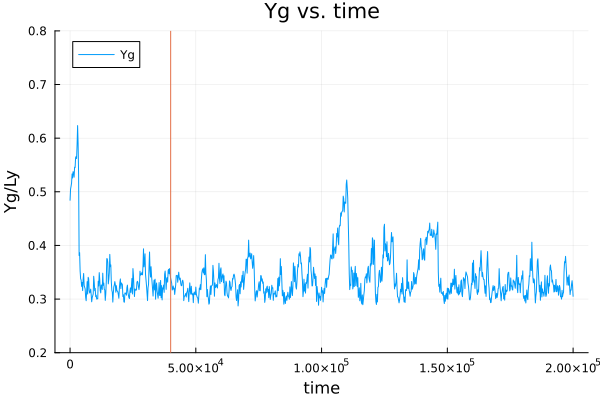
\includegraphics[width=\textwidth]{image/RaRtmap_time/2023-11-14T20:07:58.625__chi1.265_Ay50_rho0.4_T0.43_dT0.04_Rd0.0_Rt0.0_Ra0.938769_g0.0003999718779659611_run4.0e7_output.png}
      \subcaption{$\text{R}_\text{a}=0.938,\\\text{R}_\text{t}=0.0$}
      \label{}
    \end{minipage} &
    \begin{minipage}[t]{0.2\hsize}
      \centering
      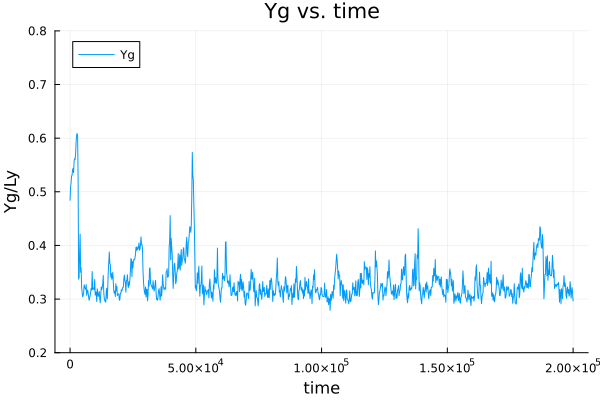
\includegraphics[width=\textwidth]{image/RaRtmap_time/2023-11-14T21:01:09.992__chi1.265_Ay50_rho0.4_T0.43_dT0.04_Rd0.0_Rt0.0_Ra1.4081535_g0.0003999718779659611_run4.0e7_output.png}
      \subcaption{$\text{R}_\text{a}=1.408,\\\text{R}_\text{t}=0.0$}
      \label{}
    \end{minipage} &
    \begin{minipage}[t]{0.2\hsize}
      \centering
      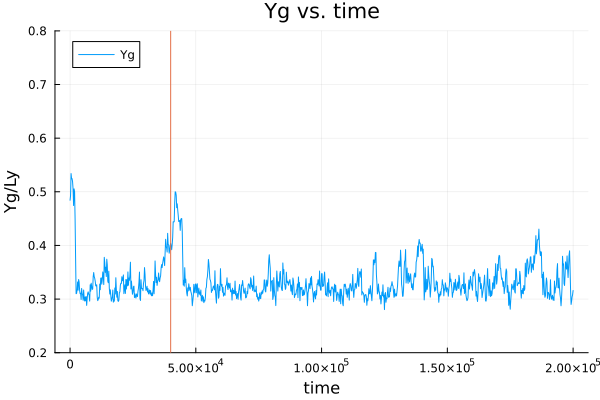
\includegraphics[width=\textwidth]{image/RaRtmap_time/2023-11-14T21:54:59.835__chi1.265_Ay50_rho0.4_T0.43_dT0.04_Rd0.0_Rt0.0_Ra1.877538_g0.0003999718779659611_run4.0e7_output.png}
      \subcaption{$\text{R}_\text{a}=1.877,\\\text{R}_\text{t}=0.0$}
      \label{}
    \end{minipage} \\
    \begin{minipage}[t]{0.2\hsize}
      \centering
      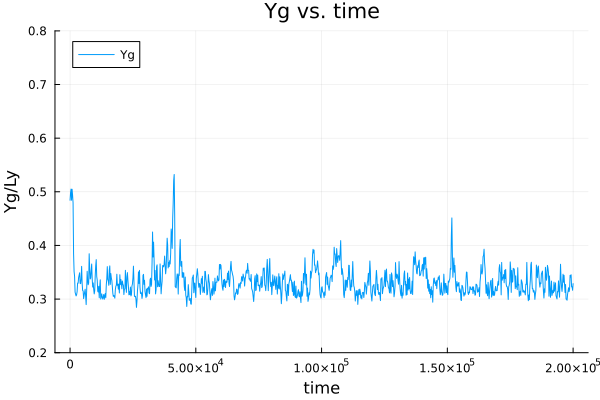
\includegraphics[width=\textwidth]{image/RaRtmap_time/2023-11-14T22:51:24.191__chi1.265_Ay50_rho0.4_T0.43_dT0.04_Rd0.0_Rt0.125_Ra0.0_g0.0003999718779659611_run4.0e7_output.png}
      \subcaption{$\text{R}_\text{a}=0.0,\\\text{R}_\text{t}=0.125$}
      \label{}
    \end{minipage} &
    \begin{minipage}[t]{0.2\hsize}
      \centering
      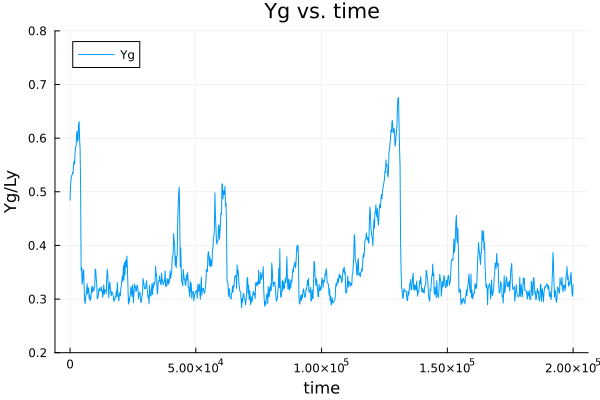
\includegraphics[width=\textwidth]{image/RaRtmap_time/2023-11-14T23:48:31.439__chi1.265_Ay50_rho0.4_T0.43_dT0.04_Rd0.0_Rt0.125_Ra0.4693845_g0.0003999718779659611_run4.0e7_output.png}
      \subcaption{$\text{R}_\text{a}=0.469,\\\text{R}_\text{t}=0.125$}
      \label{}
    \end{minipage} &
    \begin{minipage}[t]{0.2\hsize}
      \centering
      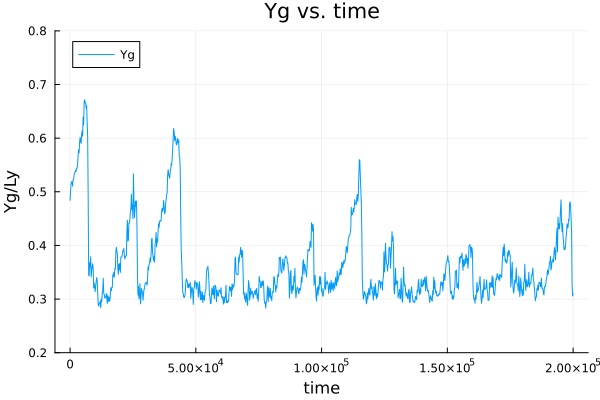
\includegraphics[width=\textwidth]{image/RaRtmap_time/2023-11-15T00:43:33.781__chi1.265_Ay50_rho0.4_T0.43_dT0.04_Rd0.0_Rt0.125_Ra0.938769_g0.0003999718779659611_run4.0e7_output.png}
      \subcaption{$\text{R}_\text{a}=0.938,\\\text{R}_\text{t}=0.125$}
      \label{}
    \end{minipage} &
    \begin{minipage}[t]{0.2\hsize}
      \centering
      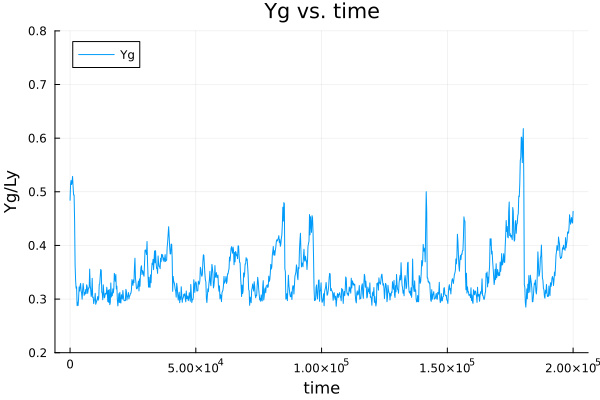
\includegraphics[width=\textwidth]{image/RaRtmap_time/2023-11-15T01:35:17.404__chi1.265_Ay50_rho0.4_T0.43_dT0.04_Rd0.0_Rt0.125_Ra1.4081535_g0.0003999718779659611_run4.0e7_output.png}
      \subcaption{$\text{R}_\text{a}=1.408,\\\text{R}_\text{t}=0.125$}
      \label{}
    \end{minipage} &
    \begin{minipage}[t]{0.2\hsize}
      \centering
      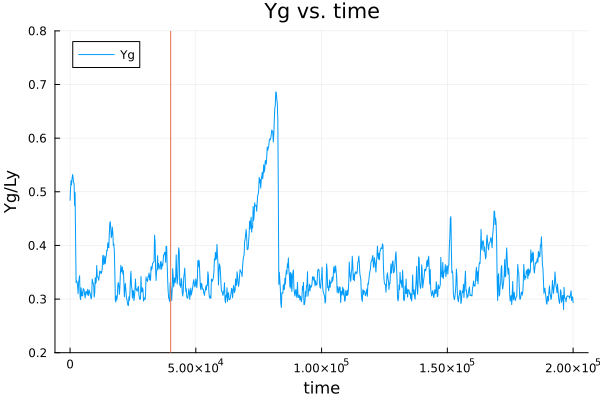
\includegraphics[width=\textwidth]{image/RaRtmap_time/2023-11-15T02:27:34.337__chi1.265_Ay50_rho0.4_T0.43_dT0.04_Rd0.0_Rt0.125_Ra1.877538_g0.0003999718779659611_run4.0e7_output.png}
      \subcaption{$\text{R}_\text{a}=1.877,\\\text{R}_\text{t}=0.125$}
      \label{}
    \end{minipage} \\
    \begin{minipage}[t]{0.2\hsize}
      \centering
      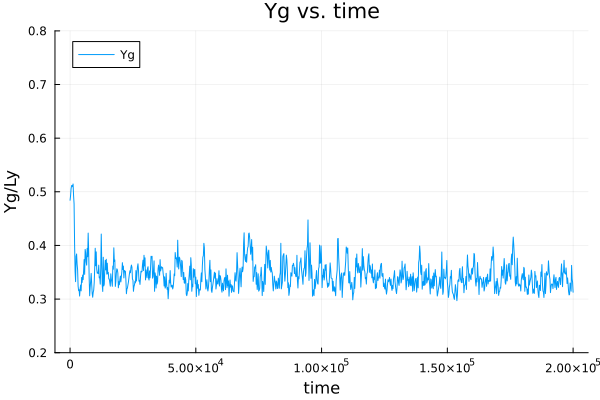
\includegraphics[width=\textwidth]{image/RaRtmap_time/2023-11-15T03:19:32.715__chi1.265_Ay50_rho0.4_T0.43_dT0.04_Rd0.0_Rt0.25_Ra0.0_g0.0003999718779659611_run4.0e7_output.png}
      \subcaption{$\text{R}_\text{a}=0.0,\\\text{R}_\text{t}=0.250$}
      \label{}
    \end{minipage} &
    \begin{minipage}[t]{0.2\hsize}
      \centering
      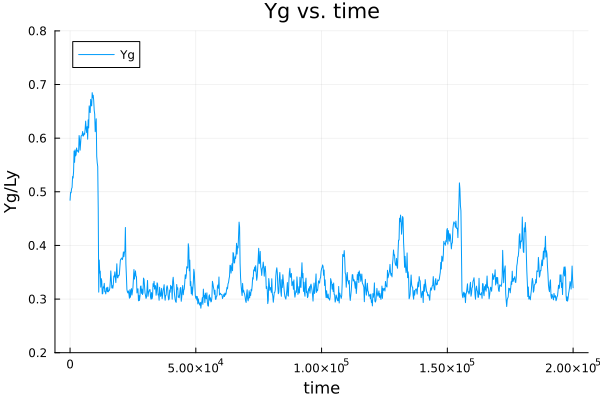
\includegraphics[width=\textwidth]{image/RaRtmap_time/2023-11-15T04:11:00.956__chi1.265_Ay50_rho0.4_T0.43_dT0.04_Rd0.0_Rt0.25_Ra0.4693845_g0.0003999718779659611_run4.0e7_output.png}
      \subcaption{$\text{R}_\text{a}=0.469,\\\text{R}_\text{t}=0.250$}
      \label{}
    \end{minipage} &
    \begin{minipage}[t]{0.2\hsize}
      \centering
      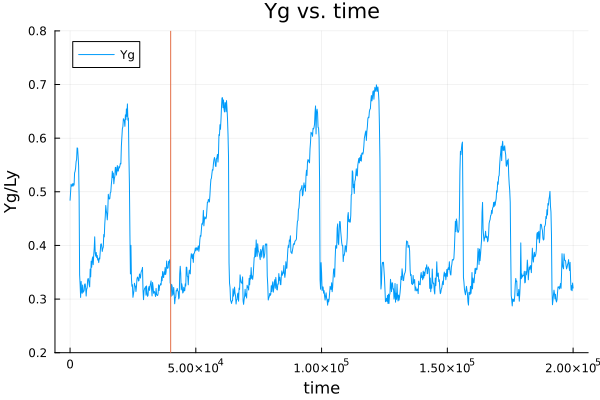
\includegraphics[width=\textwidth]{image/RaRtmap_time/2023-11-15T05:03:45.973__chi1.265_Ay50_rho0.4_T0.43_dT0.04_Rd0.0_Rt0.25_Ra0.938769_g0.0003999718779659611_run4.0e7_output.png}
      \subcaption{$\text{R}_\text{a}=0.938,\\\text{R}_\text{t}=0.250$}
      \label{}
    \end{minipage} &
    \begin{minipage}[t]{0.2\hsize}
      \centering
      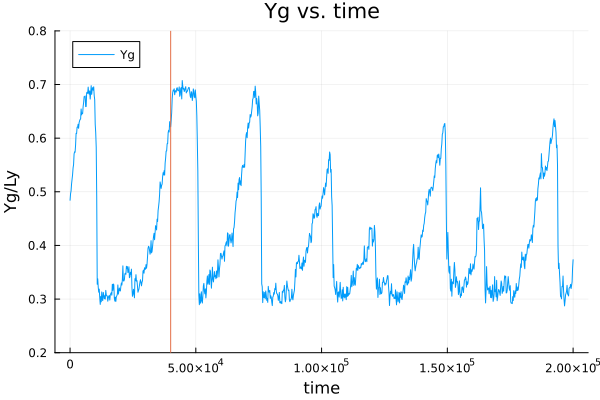
\includegraphics[width=\textwidth]{image/RaRtmap_time/2023-11-15T05:53:00.667__chi1.265_Ay50_rho0.4_T0.43_dT0.04_Rd0.0_Rt0.25_Ra1.4081535_g0.0003999718779659611_run4.0e7_output.png}
      \subcaption{$\text{R}_\text{a}=1.408,\\\text{R}_\text{t}=0.250$}
      \label{}
    \end{minipage} &
    \begin{minipage}[t]{0.2\hsize}
      \centering
      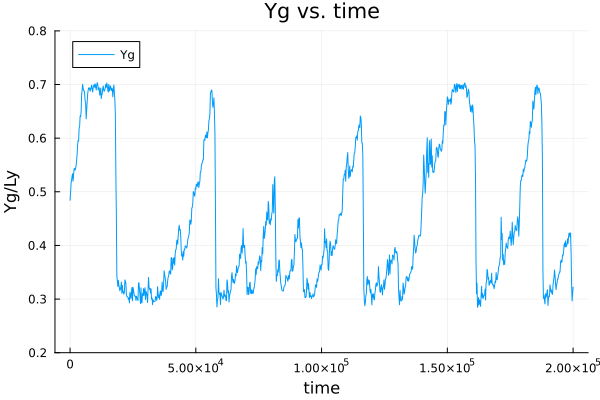
\includegraphics[width=\textwidth]{image/RaRtmap_time/2023-11-15T06:43:21.554__chi1.265_Ay50_rho0.4_T0.43_dT0.04_Rd0.0_Rt0.25_Ra1.877538_g0.0003999718779659611_run4.0e7_output.png}
      \subcaption{$\text{R}_\text{a}=1.877,\\\text{R}_\text{t}=0.250$}
      \label{}
    \end{minipage} \\
    \begin{minipage}[t]{0.2\hsize}
      \centering
      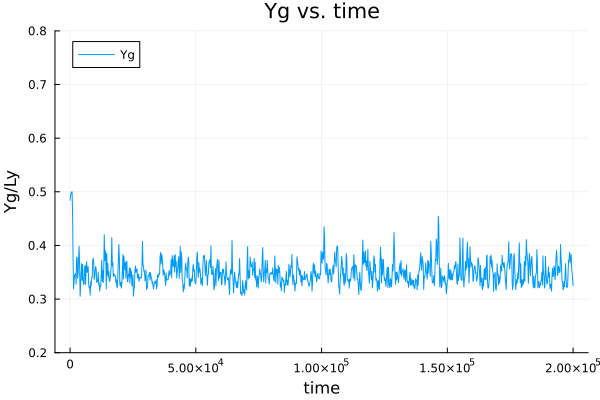
\includegraphics[width=\textwidth]{image/RaRtmap_time/2023-11-15T07:34:00.555__chi1.265_Ay50_rho0.4_T0.43_dT0.04_Rd0.0_Rt0.375_Ra0.0_g0.0003999718779659611_run4.0e7_output.png}
      \subcaption{$\text{R}_\text{a}=0.0,\\\text{R}_\text{t}=0.375$}
      \label{}
    \end{minipage} &
    \begin{minipage}[t]{0.2\hsize}
      \centering
      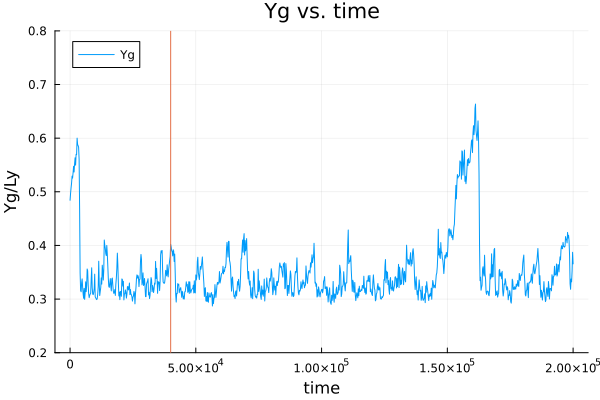
\includegraphics[width=\textwidth]{image/RaRtmap_time/2023-11-15T08:24:37.362__chi1.265_Ay50_rho0.4_T0.43_dT0.04_Rd0.0_Rt0.375_Ra0.4693845_g0.0003999718779659611_run4.0e7_output.png}
      \subcaption{$\text{R}_\text{a}=0.469,\\\text{R}_\text{t}=0.375$}
      \label{}
    \end{minipage} &
    \begin{minipage}[t]{0.2\hsize}
      \centering
      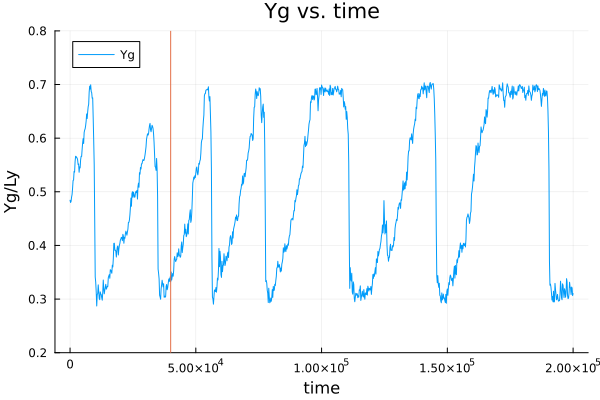
\includegraphics[width=\textwidth]{image/RaRtmap_time/2023-11-15T09:16:40.082__chi1.265_Ay50_rho0.4_T0.43_dT0.04_Rd0.0_Rt0.375_Ra0.938769_g0.0003999718779659611_run4.0e7_output.png}
      \subcaption{$\text{R}_\text{a}=0.938,\\\text{R}_\text{t}=0.375$}
      \label{}
    \end{minipage} &
    \begin{minipage}[t]{0.2\hsize}
      \centering
      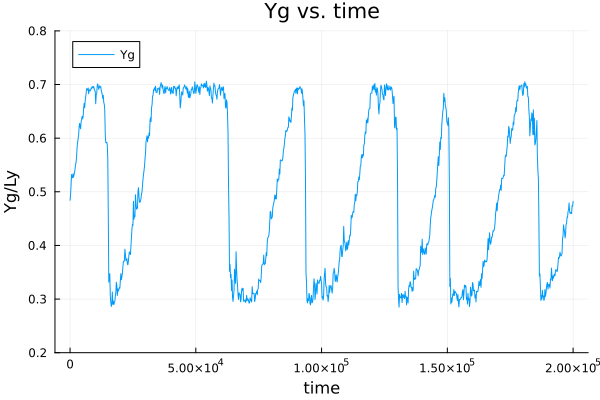
\includegraphics[width=\textwidth]{image/RaRtmap_time/2023-11-15T10:07:20.945__chi1.265_Ay50_rho0.4_T0.43_dT0.04_Rd0.0_Rt0.375_Ra1.4081535_g0.0003999718779659611_run4.0e7_output.png}
      \subcaption{$\text{R}_\text{a}=1.408,\\\text{R}_\text{t}=0.375$}
      \label{}
    \end{minipage} &
    \begin{minipage}[t]{0.2\hsize}
      \centering
      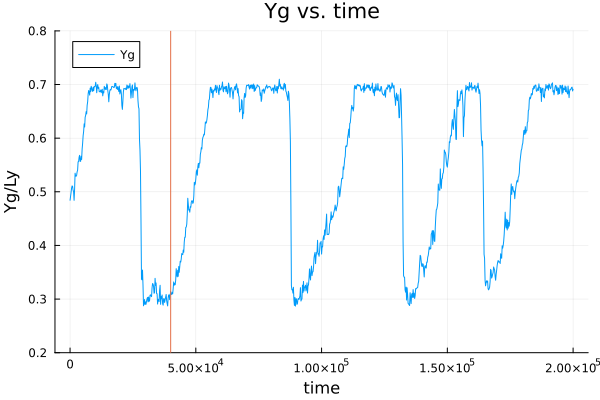
\includegraphics[width=\textwidth]{image/RaRtmap_time/2023-11-15T10:59:30.665__chi1.265_Ay50_rho0.4_T0.43_dT0.04_Rd0.0_Rt0.375_Ra1.877538_g0.0003999718779659611_run4.0e7_output.png}
      \subcaption{$\text{R}_\text{a}=1.877,\\\text{R}_\text{t}=0.375$}
      \label{}
    \end{minipage} \\
    \begin{minipage}[t]{0.2\hsize}
      \centering
      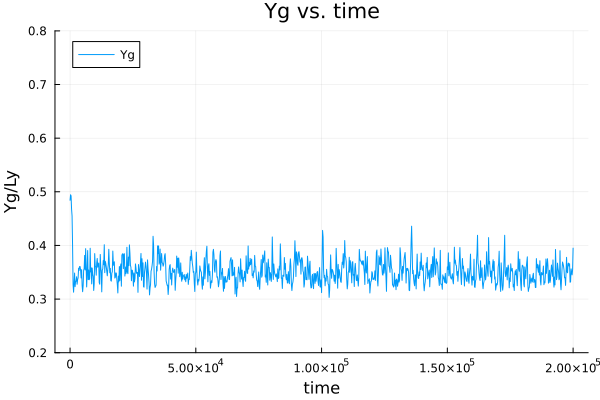
\includegraphics[width=\textwidth]{image/RaRtmap_time/2023-11-15T11:53:37.697__chi1.265_Ay50_rho0.4_T0.43_dT0.04_Rd0.0_Rt0.5_Ra0.0_g0.0003999718779659611_run4.0e7_output.png}
      \subcaption{$\text{R}_\text{a}=0.0,\\\text{R}_\text{t}=0.500$}
      \label{}
    \end{minipage} &
    \begin{minipage}[t]{0.2\hsize}
      \centering
      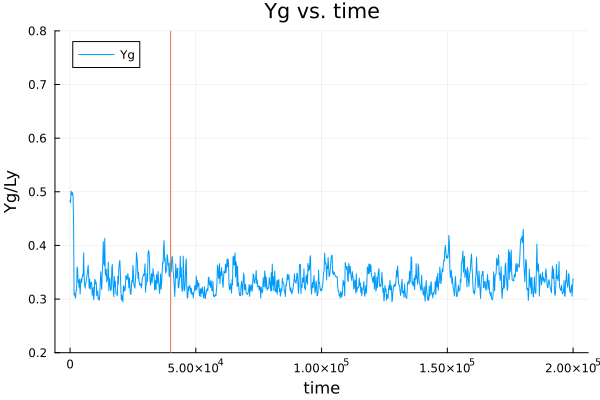
\includegraphics[width=\textwidth]{image/RaRtmap_time/2023-11-15T12:45:26.303__chi1.265_Ay50_rho0.4_T0.43_dT0.04_Rd0.0_Rt0.5_Ra0.4693845_g0.0003999718779659611_run4.0e7_output.png}
      \subcaption{$\text{R}_\text{a}=0.469,\\\text{R}_\text{t}=0.500$}
      \label{fig:RaRtmap_time_Ra0.469_Rt0.500}
    \end{minipage} &
    \begin{minipage}[t]{0.2\hsize}
      \centering
      \includegraphics[width=\textwidth]{image/RaRtmap_time/2023-11-15T13:37:58.058__chi1.265_Ay50_rho0.4_T0.43_dT0.04_Rd0.0_Rt0.5_Ra0.938769_g0.0003999718779659611_run4.0e7_output.png}
      \subcaption{$\text{R}_\text{a}=0.938,\\\text{R}_\text{t}=0.500$}
      \label{fig:RaRtmap_time_Ra0.938_Rt0.500}
    \end{minipage} &
    \begin{minipage}[t]{0.2\hsize}
      \centering
      \includegraphics[width=\textwidth]{image/RaRtmap_time/2023-11-15T14:30:22.529__chi1.265_Ay50_rho0.4_T0.43_dT0.04_Rd0.0_Rt0.5_Ra1.4081535_g0.0003999718779659611_run4.0e7_output.png}
      \subcaption{$\text{R}_\text{a}=1.408,\\\text{R}_\text{t}=0.500$}
      \label{}
    \end{minipage} &
    \begin{minipage}[t]{0.2\hsize}
      \centering
      \includegraphics[width=\textwidth]{image/RaRtmap_time/2023-11-15T15:21:59.073__chi1.265_Ay50_rho0.4_T0.43_dT0.04_Rd0.0_Rt0.5_Ra1.877538_g0.0003999718779659611_run4.0e7_output.png}
      \subcaption{$\text{R}_\text{a}=1.877,\\\text{R}_\text{t}=0.500$}
      \label{}
    \end{minipage} 
  \end{tabular}
  \caption{$t_i = 0, t_f = 2.0 \times 10^5, \dd t \sqrt{\varepsilon / m \sigma^2}= 0.005, t \sqrt{\varepsilon / m \sigma^2} = 200 ごとにプロット.$}
  \label{fig:RaRtmap_time}
\end{figure}


図\ref{fig:RaRtmap_time}では, 初期条件から$t_f \sqrt{\varepsilon / m \sigma^2} = 2.0 \times 10^{5}$までの時間変化をプロットしており, 赤い線の時刻($t \sqrt{\varepsilon / m \sigma^2}= 4.0 \times 10^4$)あたりで定常状態に到達していると判断した. 図\ref{fig:RaRtmap_time}を見ると, 引力幅$\text{R}_\text{a}=0.0$の時は, ある定常状態のまわりのランダムなゆらぎが観測されているが, $\text{R}_\text{a} \ge 0.469, \text{R}_\text{t} \ge 0.125$の時は決してランダムとは言えない. $\text{R}_\text{a} \ge 0.938 かつ\text{R}_\text{t} \ge 0.250$の時には周期的なダイナミクスが発生していることが見てとれる. 

\section{重力を先にかけて, 熱流を後からかける}\label{sec:RaRtmap_drop}

初期条件が異なる場合にダイナミクスが変化するかを調べるために, 重力と熱流をかけるタイミングをずらしたシミュレーションを設定した. まず, $t \sqrt{\varepsilon / m \sigma^2} = 2.0 \times 10^{5}$の時点まで重力のみをかけて, 粒子集団が落ちきってから熱流をかける. 

\begin{itemize}
  \item $N = 1250$
  \item $\rho \sigma^2 = 0.4$
  \item $L_x / \sigma \simeq 79.0$
  \item $L_y / \sigma \simeq 158.1$
  \item $k_{\text{B}} T/\varepsilon = 4.3$
  \item $k_{\text{B}} \Delta T/\varepsilon = 0.0$
  \item $mg\sigma/\varepsilon \simeq 2.0 \times 10^{-4}$
\end{itemize}

温度差のある熱浴をそれぞれ改めて以下のようにつけ, 熱流をかけてシミュレーションを続ける. 熱流をかけ始めてから, 定常状態に至るまでの時間を\ref{sec:RaRtmap}節と同様に$t \sqrt{\varepsilon / m \sigma^2} = 4.0 \times 10^{4}$として, 重力をかけ始めてから数えて$t \sqrt{\varepsilon / m \sigma^2} = 2.4 \times 10^{5}$の時点で定常状態に到達していると考える. 

\begin{itemize}
  \item $\chi = k_{\text{B}}\Delta T / mg L_y = 1.265$
  \item $k_{\text{B}} \Delta T/\varepsilon = 0.04$
  \item $t_i \sqrt{\varepsilon / m \sigma^2} = 2.4 \times 10^{5}$
  \item $t_f \sqrt{\varepsilon / m \sigma^2} = 4.0 \times 10^{5}$
\end{itemize}

\begin{figure}[H]
  \centering
  \includegraphics[scale=0.6]{image/RaRtmap_drop_time/2023-12-21T10:44:56.628_RaRtmap_chi1.265_Ay50_rho0.4_T0.43_dT0.04_Rd0.0_Rt0.0_Ra0.0_g0.0003999718779659611_run4.0e7.png}
  \label{}
  \caption{$\text{R}_\text{a}=0.0,\text{R}_\text{t}=0.0$}
\end{figure}

\begin{figure}[H]
  \begin{tabular}{ccccc}
    \begin{minipage}[t]{0.2\hsize}
      \centering
      \includegraphics[width=\textwidth]{image/RaRtmap_drop_time/2023-12-21T10:44:56.628_RaRtmap_chi1.265_Ay50_rho0.4_T0.43_dT0.04_Rd0.0_Rt0.0_Ra0.0_g0.0003999718779659611_run4.0e7.png}
      \subcaption{$\text{R}_\text{a}=0.0,\\\text{R}_\text{t}=0.0$}
      \label{fig:RaRtmap_drop_time_Ra0.0_Rt0.0}
    \end{minipage} &
    \begin{minipage}[t]{0.2\hsize}
      \centering
      \includegraphics[width=\textwidth]{image/RaRtmap_drop_time/2023-12-21T10:44:57.232_RaRtmap_chi1.265_Ay50_rho0.4_T0.43_dT0.04_Rd0.0_Rt0.0_Ra0.4693845_g0.0003999718779659611_run4.0e7.png}
      \subcaption{$\text{R}_\text{a}=0.469,\\\text{R}_\text{t}=0.0$}
      \label{}
    \end{minipage} &
    \begin{minipage}[t]{0.2\hsize}
      \centering
      \includegraphics[width=\textwidth]{image/RaRtmap_drop_time/2023-12-21T10:44:57.302_RaRtmap_chi1.265_Ay50_rho0.4_T0.43_dT0.04_Rd0.0_Rt0.0_Ra0.938769_g0.0003999718779659611_run4.0e7.png}
      \subcaption{$\text{R}_\text{a}=0.938,\\\text{R}_\text{t}=0.0$}
      \label{}
    \end{minipage} &
    \begin{minipage}[t]{0.2\hsize}
      \centering
      \includegraphics[width=\textwidth]{image/RaRtmap_drop_time/2023-12-21T10:44:57.379_RaRtmap_chi1.265_Ay50_rho0.4_T0.43_dT0.04_Rd0.0_Rt0.0_Ra1.4081535_g0.0003999718779659611_run4.0e7.png}
      \subcaption{$\text{R}_\text{a}=1.408,\\\text{R}_\text{t}=0.0$}
      \label{}
    \end{minipage} &
    \begin{minipage}[t]{0.2\hsize}
      \centering
      \includegraphics[width=\textwidth]{image/RaRtmap_drop_time/2023-12-21T10:44:57.455_RaRtmap_chi1.265_Ay50_rho0.4_T0.43_dT0.04_Rd0.0_Rt0.0_Ra1.877538_g0.0003999718779659611_run4.0e7.png}
      \subcaption{$\text{R}_\text{a}=1.877,\\\text{R}_\text{t}=0.0$}
      \label{}
    \end{minipage} \\
    \begin{minipage}[t]{0.2\hsize}
      \centering
      \includegraphics[width=\textwidth]{image/RaRtmap_drop_time/2023-12-21T10:44:57.529_RaRtmap_chi1.265_Ay50_rho0.4_T0.43_dT0.04_Rd0.0_Rt0.125_Ra0.0_g0.0003999718779659611_run4.0e7.png}
      \subcaption{$\text{R}_\text{a}=0.0,\\\text{R}_\text{t}=0.125$}
      \label{}
    \end{minipage} &
    \begin{minipage}[t]{0.2\hsize}
      \centering
      \includegraphics[width=\textwidth]{image/RaRtmap_drop_time/2023-12-21T10:44:57.600_RaRtmap_chi1.265_Ay50_rho0.4_T0.43_dT0.04_Rd0.0_Rt0.125_Ra0.4693845_g0.0003999718779659611_run4.0e7.png}
      \subcaption{$\text{R}_\text{a}=0.469,\\\text{R}_\text{t}=0.125$}
      \label{}
    \end{minipage} &
    \begin{minipage}[t]{0.2\hsize}
      \centering
      \includegraphics[width=\textwidth]{image/RaRtmap_drop_time/2023-12-21T10:44:57.672_RaRtmap_chi1.265_Ay50_rho0.4_T0.43_dT0.04_Rd0.0_Rt0.125_Ra0.938769_g0.0003999718779659611_run4.0e7.png}
      \subcaption{$\text{R}_\text{a}=0.938,\\\text{R}_\text{t}=0.125$}
      \label{}
    \end{minipage} &
    \begin{minipage}[t]{0.2\hsize}
      \centering
      \includegraphics[width=\textwidth]{image/RaRtmap_drop_time/2023-12-21T10:44:57.746_RaRtmap_chi1.265_Ay50_rho0.4_T0.43_dT0.04_Rd0.0_Rt0.125_Ra1.4081535_g0.0003999718779659611_run4.0e7.png}
      \subcaption{$\text{R}_\text{a}=1.408,\\\text{R}_\text{t}=0.125$}
      \label{}
    \end{minipage} &
    \begin{minipage}[t]{0.2\hsize}
      \centering
      \includegraphics[width=\textwidth]{image/RaRtmap_drop_time/2023-12-21T10:44:57.821_RaRtmap_chi1.265_Ay50_rho0.4_T0.43_dT0.04_Rd0.0_Rt0.125_Ra1.877538_g0.0003999718779659611_run4.0e7.png}
      \subcaption{$\text{R}_\text{a}=1.877,\\\text{R}_\text{t}=0.125$}
      \label{}
    \end{minipage} \\
    \begin{minipage}[t]{0.2\hsize}
      \centering
      \includegraphics[width=\textwidth]{image/RaRtmap_drop_time/2023-12-21T10:44:57.897_RaRtmap_chi1.265_Ay50_rho0.4_T0.43_dT0.04_Rd0.0_Rt0.25_Ra0.0_g0.0003999718779659611_run4.0e7.png}
      \subcaption{$\text{R}_\text{a}=0.0,\\\text{R}_\text{t}=0.250$}
      \label{}
    \end{minipage} &
    \begin{minipage}[t]{0.2\hsize}
      \centering
      \includegraphics[width=\textwidth]{image/RaRtmap_drop_time/2023-12-21T10:44:57.979_RaRtmap_chi1.265_Ay50_rho0.4_T0.43_dT0.04_Rd0.0_Rt0.25_Ra0.4693845_g0.0003999718779659611_run4.0e7.png}
      \subcaption{$\text{R}_\text{a}=0.469,\\\text{R}_\text{t}=0.250$}
      \label{}
    \end{minipage} &
    \begin{minipage}[t]{0.2\hsize}
      \centering
      \includegraphics[width=\textwidth]{image/RaRtmap_drop_time/2023-12-21T10:44:58.051_RaRtmap_chi1.265_Ay50_rho0.4_T0.43_dT0.04_Rd0.0_Rt0.25_Ra0.938769_g0.0003999718779659611_run4.0e7.png}
      \subcaption{$\text{R}_\text{a}=0.938,\\\text{R}_\text{t}=0.250$}
      \label{}
    \end{minipage} &
    \begin{minipage}[t]{0.2\hsize}
      \centering
      \includegraphics[width=\textwidth]{image/RaRtmap_drop_time/2023-12-21T10:44:58.129_RaRtmap_chi1.265_Ay50_rho0.4_T0.43_dT0.04_Rd0.0_Rt0.25_Ra1.4081535_g0.0003999718779659611_run4.0e7.png}
      \subcaption{$\text{R}_\text{a}=1.408,\\\text{R}_\text{t}=0.250$}
      \label{}
    \end{minipage} &
    \begin{minipage}[t]{0.2\hsize}
      \centering
      \includegraphics[width=\textwidth]{image/RaRtmap_drop_time/2023-12-21T10:44:58.197_RaRtmap_chi1.265_Ay50_rho0.4_T0.43_dT0.04_Rd0.0_Rt0.25_Ra1.877538_g0.0003999718779659611_run4.0e7.png}
      \subcaption{$\text{R}_\text{a}=1.877,\\\text{R}_\text{t}=0.250$}
      \label{}
    \end{minipage} \\
    \begin{minipage}[t]{0.2\hsize}
      \centering
      \includegraphics[width=\textwidth]{image/RaRtmap_drop_time/2023-12-21T10:44:58.258_RaRtmap_chi1.265_Ay50_rho0.4_T0.43_dT0.04_Rd0.0_Rt0.375_Ra0.0_g0.0003999718779659611_run4.0e7.png}
      \subcaption{$\text{R}_\text{a}=0.0,\\\text{R}_\text{t}=0.375$}
      \label{}
    \end{minipage} &
    \begin{minipage}[t]{0.2\hsize}
      \centering
      \includegraphics[width=\textwidth]{image/RaRtmap_drop_time/2023-12-21T10:44:58.322_RaRtmap_chi1.265_Ay50_rho0.4_T0.43_dT0.04_Rd0.0_Rt0.375_Ra0.4693845_g0.0003999718779659611_run4.0e7.png}
      \subcaption{$\text{R}_\text{a}=0.469,\\\text{R}_\text{t}=0.375$}
      \label{}
    \end{minipage} &
    \begin{minipage}[t]{0.2\hsize}
      \centering
      \includegraphics[width=\textwidth]{image/RaRtmap_drop_time/2023-12-21T10:44:58.387_RaRtmap_chi1.265_Ay50_rho0.4_T0.43_dT0.04_Rd0.0_Rt0.375_Ra0.938769_g0.0003999718779659611_run4.0e7.png}
      \subcaption{$\text{R}_\text{a}=0.938,\\\text{R}_\text{t}=0.375$}
      \label{}
    \end{minipage} &
    \begin{minipage}[t]{0.2\hsize}
      \centering
      \includegraphics[width=\textwidth]{image/RaRtmap_drop_time/2023-12-21T10:44:58.471_RaRtmap_chi1.265_Ay50_rho0.4_T0.43_dT0.04_Rd0.0_Rt0.375_Ra1.4081535_g0.0003999718779659611_run4.0e7.png}
      \subcaption{$\text{R}_\text{a}=1.408,\\\text{R}_\text{t}=0.375$}
      \label{}
    \end{minipage} &
    \begin{minipage}[t]{0.2\hsize}
      \centering
      \includegraphics[width=\textwidth]{image/RaRtmap_drop_time/2023-12-21T10:44:58.541_RaRtmap_chi1.265_Ay50_rho0.4_T0.43_dT0.04_Rd0.0_Rt0.375_Ra1.877538_g0.0003999718779659611_run4.0e7.png}
      \subcaption{$\text{R}_\text{a}=1.877,\\\text{R}_\text{t}=0.375$}
      \label{}
    \end{minipage} \\
    \begin{minipage}[t]{0.2\hsize}
      \centering
      \includegraphics[width=\textwidth]{image/RaRtmap_drop_time/2023-12-21T10:44:58.621_RaRtmap_chi1.265_Ay50_rho0.4_T0.43_dT0.04_Rd0.0_Rt0.5_Ra0.0_g0.0003999718779659611_run4.0e7.png}
      \subcaption{$\text{R}_\text{a}=0.0,\\\text{R}_\text{t}=0.500$}
      \label{}
    \end{minipage} &
    \begin{minipage}[t]{0.2\hsize}
      \centering
      \includegraphics[width=\textwidth]{image/RaRtmap_drop_time/2023-12-21T10:44:58.706_RaRtmap_chi1.265_Ay50_rho0.4_T0.43_dT0.04_Rd0.0_Rt0.5_Ra0.4693845_g0.0003999718779659611_run4.0e7.png}
      \subcaption{$\text{R}_\text{a}=0.469,\\\text{R}_\text{t}=0.500$}
      \label{fig:RaRtmap_drop_time_Ra0.469_Rt0.500}
    \end{minipage} &
    \begin{minipage}[t]{0.2\hsize}
      \centering
      \includegraphics[width=\textwidth]{image/RaRtmap_drop_time/2023-12-21T10:44:58.788_RaRtmap_chi1.265_Ay50_rho0.4_T0.43_dT0.04_Rd0.0_Rt0.5_Ra0.938769_g0.0003999718779659611_run4.0e7.png}
      \subcaption{$\text{R}_\text{a}=0.938,\\\text{R}_\text{t}=0.500$}
      \label{fig:RaRtmap_drop_time_Ra0.938_Rt0.500}
    \end{minipage} &
    \begin{minipage}[t]{0.2\hsize}
      \centering
      \includegraphics[width=\textwidth]{image/RaRtmap_drop_time/2023-12-21T10:44:58.872_RaRtmap_chi1.265_Ay50_rho0.4_T0.43_dT0.04_Rd0.0_Rt0.5_Ra1.4081535_g0.0003999718779659611_run4.0e7.png}
      \subcaption{$\text{R}_\text{a}=1.408,\\\text{R}_\text{t}=0.500$}
      \label{}
    \end{minipage} &
    \begin{minipage}[t]{0.2\hsize}
      \centering
      \includegraphics[width=\textwidth]{image/RaRtmap_drop_time/2023-12-21T10:44:58.955_RaRtmap_chi1.265_Ay50_rho0.4_T0.43_dT0.04_Rd0.0_Rt0.5_Ra1.877538_g0.0003999718779659611_run4.0e7.png}
      \subcaption{$\text{R}_\text{a}=1.877,\\\text{R}_\text{t}=0.500$}
      \label{}
    \end{minipage} 
  \end{tabular}
  \caption{$t_i = 2.4 \times 10^5, t_f = 4.0 \times 10^5, \dd t \sqrt{\varepsilon / m \sigma^2}= 0.005, t \sqrt{\varepsilon / m \sigma^2} = 200 ごとにプロット.$}
  \label{fig:RaRtmap_drop_time}
\end{figure}


\ref{sec:RaRtmap}節と同様に, 図\ref{fig:RaRtmap_drop_time}を見たとき, 引力幅$\text{R}_\text{a}=0.0$の時は, ある定常状態のまわりのランダムなゆらぎが観測されているが, $\text{R}_\text{a} \ge 0.469, \text{R}_\text{t} \ge 0.125$の時は決してランダムとは言えない. $\text{R}_\text{a} \ge 0.938 かつ\text{R}_\text{t} \ge 0.250$の時には周期的なダイナミクスが発生していることが見てとれる.  

このことより, 重力と熱流をかけるタイミングをずらしたとしてもダイナミクスは大きく変わらないことが分かる. 

図\ref{fig:RaRtmap_time}, \ref{fig:RaRtmap_drop_time}の (x), (y) に注目すると, \ref{sec:RaRtmap}節でのそれと比べて, 上壁に張りついている時間が長い様子が見てとれる. 周期的なダイナミクスが発生しているのかどうか, \ref{sec:RaRtmap10}節では, \ref{sec:RaRtmap10}の10倍の時間をとって実験をする. 

\section{重力のみをかける}\label{sec:dT0}

重力のみをかけた系, 熱流のみをかけた系を考えると, それぞれ流体系は壁の下部, 上部で安定することが予想できたが, 実際に実験で確かめた. 

まず, 重力のみをかけた系であるが, $t \sqrt{\varepsilon / m \sigma^2}= 4.0 \times 10^4$の時点で定常状態に到達していると考える. 

\begin{itemize}
  \item $N = 1250$
  \item $\rho {\sigma}^2 = 0.4$
  \item $L_x / \sigma \simeq 39.5$
  \item $L_y / \sigma \simeq 79.0$
  \item $k_{\text{B}} T / \varepsilon = 0.43$
  \item $k_{\text{B}} \Delta T / \varepsilon = 0.0$
  \item $mg\sigma/\varepsilon \simeq 4.0 \times 10^{-4}$
  \item $t_i \sqrt{\varepsilon / m \sigma^2}= 4.0 \times 10^4$
  \item $t_f \sqrt{\varepsilon / m \sigma^2} = 2.0 \times 10^{5}$
\end{itemize}


\begin{figure}[H]
  \begin{tabular}{ccccc}
    \begin{minipage}[t]{0.2\hsize}
      \centering
      \includegraphics[width=\textwidth]{image/dT0_time/2024-01-15T14:30:46.366_mapg0_chi0_Ay50_rho0.4_T0.43_dT0.0_Rd0.0_Rt0.0_Ra0.0_g0.0003999718779659611_run4.0e7.png}
      \subcaption{$\text{R}_\text{a}=0.0,\text{R}_\text{t}=0.0$}
      \label{fig:dT0_time_Ra0.0_Rt0.0}
    \end{minipage} &
    \begin{minipage}[t]{0.2\hsize}
      \centering
      \includegraphics[width=\textwidth]{image/dT0_time/2024-01-15T14:30:46.901_mapg0_chi0_Ay50_rho0.4_T0.43_dT0.0_Rd0.0_Rt0.0_Ra0.4693845_g0.0003999718779659611_run4.0e7.png}
      \subcaption{$\text{R}_\text{a}=0.469,\\\text{R}_\text{t}=0.0$}
      \label{}
    \end{minipage} &
    \begin{minipage}[t]{0.2\hsize}
      \centering
      \includegraphics[width=\textwidth]{image/dT0_time/2024-01-15T14:30:46.968_mapg0_chi0_Ay50_rho0.4_T0.43_dT0.0_Rd0.0_Rt0.0_Ra0.938769_g0.0003999718779659611_run4.0e7.png}
      \subcaption{$\text{R}_\text{a}=0.938,\\\text{R}_\text{t}=0.0$}
      \label{}
    \end{minipage} &
    \begin{minipage}[t]{0.2\hsize}
      \centering
      \includegraphics[width=\textwidth]{image/dT0_time/2024-01-15T14:30:47.037_mapg0_chi0_Ay50_rho0.4_T0.43_dT0.0_Rd0.0_Rt0.0_Ra1.4081535_g0.0003999718779659611_run4.0e7.png}
      \subcaption{$\text{R}_\text{a}=1.408,\\\text{R}_\text{t}=0.0$}
      \label{}
    \end{minipage} &
    \begin{minipage}[t]{0.2\hsize}
      \centering
      \includegraphics[width=\textwidth]{image/dT0_time/2024-01-15T14:30:47.119_mapg0_chi0_Ay50_rho0.4_T0.43_dT0.0_Rd0.0_Rt0.0_Ra1.877538_g0.0003999718779659611_run4.0e7.png}
      \subcaption{$\text{R}_\text{a}=1.877,\\\text{R}_\text{t}=0.0$}
      \label{}
    \end{minipage} \\
    \begin{minipage}[t]{0.2\hsize}
      \centering
      \includegraphics[width=\textwidth]{image/dT0_time/2024-01-15T14:30:47.186_mapg0_chi0_Ay50_rho0.4_T0.43_dT0.0_Rd0.0_Rt0.125_Ra0.0_g0.0003999718779659611_run4.0e7.png}
      \subcaption{$\text{R}_\text{a}=0.0,\\\text{R}_\text{t}=0.125$}
      \label{}
    \end{minipage} &
    \begin{minipage}[t]{0.2\hsize}
      \centering
      \includegraphics[width=\textwidth]{image/dT0_time/2024-01-15T14:30:47.255_mapg0_chi0_Ay50_rho0.4_T0.43_dT0.0_Rd0.0_Rt0.125_Ra0.4693845_g0.0003999718779659611_run4.0e7.png}
      \subcaption{$\text{R}_\text{a}=0.469,\\\text{R}_\text{t}=0.125$}
      \label{}
    \end{minipage} &
    \begin{minipage}[t]{0.2\hsize}
      \centering
      \includegraphics[width=\textwidth]{image/dT0_time/2024-01-15T14:30:47.323_mapg0_chi0_Ay50_rho0.4_T0.43_dT0.0_Rd0.0_Rt0.125_Ra0.938769_g0.0003999718779659611_run4.0e7.png}
      \subcaption{$\text{R}_\text{a}=0.938,\\\text{R}_\text{t}=0.125$}
      \label{}
    \end{minipage} &
    \begin{minipage}[t]{0.2\hsize}
      \centering
      \includegraphics[width=\textwidth]{image/dT0_time/2024-01-15T14:30:47.390_mapg0_chi0_Ay50_rho0.4_T0.43_dT0.0_Rd0.0_Rt0.125_Ra1.4081535_g0.0003999718779659611_run4.0e7.png}
      \subcaption{$\text{R}_\text{a}=1.408,\\\text{R}_\text{t}=0.125$}
      \label{}
    \end{minipage} &
    \begin{minipage}[t]{0.2\hsize}
      \centering
      \includegraphics[width=\textwidth]{image/dT0_time/2024-01-15T14:30:47.459_mapg0_chi0_Ay50_rho0.4_T0.43_dT0.0_Rd0.0_Rt0.125_Ra1.877538_g0.0003999718779659611_run4.0e7.png}
      \subcaption{$\text{R}_\text{a}=1.877,\\\text{R}_\text{t}=0.125$}
      \label{}
    \end{minipage} \\
    \begin{minipage}[t]{0.2\hsize}
      \centering
      \includegraphics[width=\textwidth]{image/dT0_time/2024-01-15T14:30:47.525_mapg0_chi0_Ay50_rho0.4_T0.43_dT0.0_Rd0.0_Rt0.25_Ra0.0_g0.0003999718779659611_run4.0e7.png}
      \subcaption{$\text{R}_\text{a}=0.0,\\\text{R}_\text{t}=0.250$}
      \label{}
    \end{minipage} &
    \begin{minipage}[t]{0.2\hsize}
      \centering
      \includegraphics[width=\textwidth]{image/dT0_time/2024-01-15T14:30:47.592_mapg0_chi0_Ay50_rho0.4_T0.43_dT0.0_Rd0.0_Rt0.25_Ra0.4693845_g0.0003999718779659611_run4.0e7.png}
      \subcaption{$\text{R}_\text{a}=0.469,\\\text{R}_\text{t}=0.250$}
      \label{}
    \end{minipage} &
    \begin{minipage}[t]{0.2\hsize}
      \centering
      \includegraphics[width=\textwidth]{image/dT0_time/2024-01-15T14:30:47.659_mapg0_chi0_Ay50_rho0.4_T0.43_dT0.0_Rd0.0_Rt0.25_Ra0.938769_g0.0003999718779659611_run4.0e7.png}
      \subcaption{$\text{R}_\text{a}=0.938,\\\text{R}_\text{t}=0.250$}
      \label{}
    \end{minipage} &
    \begin{minipage}[t]{0.2\hsize}
      \centering
      \includegraphics[width=\textwidth]{image/dT0_time/2024-01-15T14:30:47.726_mapg0_chi0_Ay50_rho0.4_T0.43_dT0.0_Rd0.0_Rt0.25_Ra1.4081535_g0.0003999718779659611_run4.0e7.png}
      \subcaption{$\text{R}_\text{a}=1.408,\\\text{R}_\text{t}=0.250$}
      \label{}
    \end{minipage} &
    \begin{minipage}[t]{0.2\hsize}
      \centering
      \includegraphics[width=\textwidth]{image/dT0_time/2024-01-15T14:30:47.794_mapg0_chi0_Ay50_rho0.4_T0.43_dT0.0_Rd0.0_Rt0.25_Ra1.877538_g0.0003999718779659611_run4.0e7.png}
      \subcaption{$\text{R}_\text{a}=1.877,\\\text{R}_\text{t}=0.250$}
      \label{}
    \end{minipage} \\
    \begin{minipage}[t]{0.2\hsize}
      \centering
      \includegraphics[width=\textwidth]{image/dT0_time/2024-01-15T14:30:47.876_mapg0_chi0_Ay50_rho0.4_T0.43_dT0.0_Rd0.0_Rt0.375_Ra0.0_g0.0003999718779659611_run4.0e7.png}
      \subcaption{$\text{R}_\text{a}=0.0,\\\text{R}_\text{t}=0.375$}
      \label{}
    \end{minipage} &
    \begin{minipage}[t]{0.2\hsize}
      \centering
      \includegraphics[width=\textwidth]{image/dT0_time/2024-01-15T14:30:47.945_mapg0_chi0_Ay50_rho0.4_T0.43_dT0.0_Rd0.0_Rt0.375_Ra0.4693845_g0.0003999718779659611_run4.0e7.png}
      \subcaption{$\text{R}_\text{a}=0.469,\\\text{R}_\text{t}=0.375$}
      \label{}
    \end{minipage} &
    \begin{minipage}[t]{0.2\hsize}
      \centering
      \includegraphics[width=\textwidth]{image/dT0_time/2024-01-15T14:30:48.012_mapg0_chi0_Ay50_rho0.4_T0.43_dT0.0_Rd0.0_Rt0.375_Ra0.938769_g0.0003999718779659611_run4.0e7.png}
      \subcaption{$\text{R}_\text{a}=0.938,\\\text{R}_\text{t}=0.375$}
      \label{}
    \end{minipage} &
    \begin{minipage}[t]{0.2\hsize}
      \centering
      \includegraphics[width=\textwidth]{image/dT0_time/2024-01-15T14:30:48.081_mapg0_chi0_Ay50_rho0.4_T0.43_dT0.0_Rd0.0_Rt0.375_Ra1.4081535_g0.0003999718779659611_run4.0e7.png}
      \subcaption{$\text{R}_\text{a}=1.408,\\\text{R}_\text{t}=0.375$}
      \label{}
    \end{minipage} &
    \begin{minipage}[t]{0.2\hsize}
      \centering
      \includegraphics[width=\textwidth]{image/dT0_time/2024-01-15T14:30:48.147_mapg0_chi0_Ay50_rho0.4_T0.43_dT0.0_Rd0.0_Rt0.375_Ra1.877538_g0.0003999718779659611_run4.0e7.png}
      \subcaption{$\text{R}_\text{a}=1.877,\\\text{R}_\text{t}=0.375$}
      \label{}
    \end{minipage} \\
    \begin{minipage}[t]{0.2\hsize}
      \centering
      \includegraphics[width=\textwidth]{image/dT0_time/2024-01-15T14:30:48.227_mapg0_chi0_Ay50_rho0.4_T0.43_dT0.0_Rd0.0_Rt0.5_Ra0.0_g0.0003999718779659611_run4.0e7.png}
      \subcaption{$\text{R}_\text{a}=0.0,\\\text{R}_\text{t}=0.500$}
      \label{}
    \end{minipage} &
    \begin{minipage}[t]{0.2\hsize}
      \centering
      \includegraphics[width=\textwidth]{image/dT0_time/2024-01-15T14:30:48.295_mapg0_chi0_Ay50_rho0.4_T0.43_dT0.0_Rd0.0_Rt0.5_Ra0.4693845_g0.0003999718779659611_run4.0e7.png}
      \subcaption{$\text{R}_\text{a}=0.469,\\\text{R}_\text{t}=0.500$}
      \label{fig:dT0_time_Ra0.469_Rt0.500}
    \end{minipage} &
    \begin{minipage}[t]{0.2\hsize}
      \centering
      \includegraphics[width=\textwidth]{image/dT0_time/2024-01-15T14:30:48.365_mapg0_chi0_Ay50_rho0.4_T0.43_dT0.0_Rd0.0_Rt0.5_Ra0.938769_g0.0003999718779659611_run4.0e7.png}
      \subcaption{$\text{R}_\text{a}=0.938,\\\text{R}_\text{t}=0.500$}
      \label{fig:dT0_time_Ra0.938_Rt0.500}
    \end{minipage} &
    \begin{minipage}[t]{0.2\hsize}
      \centering
      \includegraphics[width=\textwidth]{image/dT0_time/2024-01-15T14:30:48.432_mapg0_chi0_Ay50_rho0.4_T0.43_dT0.0_Rd0.0_Rt0.5_Ra1.4081535_g0.0003999718779659611_run4.0e7.png}
      \subcaption{$\text{R}_\text{a}=1.408,\\\text{R}_\text{t}=0.500$}
      \label{}
    \end{minipage} &
    \begin{minipage}[t]{0.2\hsize}
      \centering
      \includegraphics[width=\textwidth]{image/dT0_time/2024-01-15T14:30:48.499_mapg0_chi0_Ay50_rho0.4_T0.43_dT0.0_Rd0.0_Rt0.5_Ra1.877538_g0.0003999718779659611_run4.0e7.png}
      \subcaption{$\text{R}_\text{a}=1.877,\\\text{R}_\text{t}=0.500$}
      \label{}
    \end{minipage} 
  \end{tabular}
  \caption{$t_i = 0, t_f = 2.0 \times 10^5, \dd t \sqrt{\varepsilon / m \sigma^2}= 0.005, t \sqrt{\varepsilon / m \sigma^2} = 200 ごとにプロット.$}
  \label{fig:dT0_time}
\end{figure}


この重心位置の推移から, 重心のみをかけた系では流体系が下部の壁まわりで安定することが確認できた. 

\section{熱流のみをかける}\label{sec:g0}

次に, 熱流のみをかけた系で実験をしたが, これも $t \sqrt{\varepsilon / m \sigma^2}= 4.0 \times 10^4$の時点で定常状態に到達していると考える. 

\begin{itemize}
  \item $N = 1250$
  \item $\rho {\sigma}^2 = 0.4$
  \item $L_x / \sigma \simeq 39.5$
  \item $L_y / \sigma \simeq 79.0$
  \item $k_{\text{B}} T / \varepsilon = 0.43$
  \item $k_{\text{B}} \Delta T / \varepsilon = 0.04$
  \item $mg\sigma/\varepsilon = 0.0$
  \item $t_i \sqrt{\varepsilon / m \sigma^2}= 4.0 \times 10^4$
  \item $t_f \sqrt{\varepsilon / m \sigma^2} = 2.0 \times 10^{5}$
\end{itemize}

\begin{figure}[H]
  \begin{tabular}{ccccc}
    \begin{minipage}[t]{0.2\hsize}
      \centering
      \includegraphics[width=\textwidth]{image/g0_time/2024-01-15T14:07:33.905_mapg0_chiinf_Ay50_rho0.4_T0.43_dT0.04_Rd0.0_Rt0.0_Ra0.0_g0_run4.0e7.png}
      \subcaption{$\text{R}_\text{a}=0.0,\\\text{R}_\text{t}=0.0$} % あとで差し替え.
      \label{fig:g0_time_Ra0.0_Rt0.0}
    \end{minipage} &
    \begin{minipage}[t]{0.2\hsize}
      \centering
      \includegraphics[width=\textwidth]{image/g0_time/2024-01-15T14:07:34.556_mapg0_chiinf_Ay50_rho0.4_T0.43_dT0.04_Rd0.0_Rt0.0_Ra0.4693845_g0_run4.0e7.png}
      \subcaption{$\text{R}_\text{a}=0.469,\\\text{R}_\text{t}=0.0$}
      \label{}
    \end{minipage} &
    \begin{minipage}[t]{0.2\hsize}
      \centering
      \includegraphics[width=\textwidth]{image/g0_time/2024-01-15T14:07:34.622_mapg0_chiinf_Ay50_rho0.4_T0.43_dT0.04_Rd0.0_Rt0.0_Ra0.938769_g0_run4.0e7.png}
      \subcaption{$\text{R}_\text{a}=0.938,\\\text{R}_\text{t}=0.0$}
      \label{}
    \end{minipage} &
    \begin{minipage}[t]{0.2\hsize}
      \centering
      \includegraphics[width=\textwidth]{image/g0_time/2024-01-15T14:07:34.689_mapg0_chiinf_Ay50_rho0.4_T0.43_dT0.04_Rd0.0_Rt0.0_Ra1.4081535_g0_run4.0e7.png}
      \subcaption{$\text{R}_\text{a}=1.408,\\\text{R}_\text{t}=0.0$}
      \label{}
    \end{minipage} &
    \begin{minipage}[t]{0.2\hsize}
      \centering
      \includegraphics[width=\textwidth]{image/g0_time/2024-01-15T14:07:34.770_mapg0_chiinf_Ay50_rho0.4_T0.43_dT0.04_Rd0.0_Rt0.0_Ra1.877538_g0_run4.0e7.png}
      \subcaption{$\text{R}_\text{a}=1.877,\\\text{R}_\text{t}=0.0$}
      \label{}
    \end{minipage} \\
    \begin{minipage}[t]{0.2\hsize}
      \centering
      \includegraphics[width=\textwidth]{image/g0_time/2024-01-15T14:07:34.852_mapg0_chiinf_Ay50_rho0.4_T0.43_dT0.04_Rd0.0_Rt0.125_Ra0.0_g0_run4.0e7.png}
      \subcaption{$\text{R}_\text{a}=0.0,\\\text{R}_\text{t}=0.125$}
      \label{}
    \end{minipage} &
    \begin{minipage}[t]{0.2\hsize}
      \centering
      \includegraphics[width=\textwidth]{image/g0_time/2024-01-15T14:07:34.918_mapg0_chiinf_Ay50_rho0.4_T0.43_dT0.04_Rd0.0_Rt0.125_Ra0.4693845_g0_run4.0e7.png}
      \subcaption{$\text{R}_\text{a}=0.469,\\\text{R}_\text{t}=0.125$}
      \label{}
    \end{minipage} &
    \begin{minipage}[t]{0.2\hsize}
      \centering
      \includegraphics[width=\textwidth]{image/g0_time/2024-01-15T14:07:34.988_mapg0_chiinf_Ay50_rho0.4_T0.43_dT0.04_Rd0.0_Rt0.125_Ra0.938769_g0_run4.0e7.png}
      \subcaption{$\text{R}_\text{a}=0.938,\\\text{R}_\text{t}=0.125$}
      \label{}
    \end{minipage} &
    \begin{minipage}[t]{0.2\hsize}
      \centering
      \includegraphics[width=\textwidth]{image/g0_time/2024-01-15T14:07:35.058_mapg0_chiinf_Ay50_rho0.4_T0.43_dT0.04_Rd0.0_Rt0.125_Ra1.4081535_g0_run4.0e7.png}
      \subcaption{$\text{R}_\text{a}=1.408,\\\text{R}_\text{t}=0.125$}
      \label{}
    \end{minipage} &
    \begin{minipage}[t]{0.2\hsize}
      \centering
      \includegraphics[width=\textwidth]{image/g0_time/2024-01-15T14:07:35.126_mapg0_chiinf_Ay50_rho0.4_T0.43_dT0.04_Rd0.0_Rt0.125_Ra1.877538_g0_run4.0e7.png}
      \subcaption{$\text{R}_\text{a}=1.877,\\\text{R}_\text{t}=0.125$}
      \label{}
    \end{minipage} \\
    \begin{minipage}[t]{0.2\hsize}
      \centering
      \includegraphics[width=\textwidth]{image/g0_time/2024-01-15T14:07:35.195_mapg0_chiinf_Ay50_rho0.4_T0.43_dT0.04_Rd0.0_Rt0.25_Ra0.0_g0_run4.0e7.png}
      \subcaption{$\text{R}_\text{a}=0.0,\\\text{R}_\text{t}=0.250$}
      \label{}
    \end{minipage} &
    \begin{minipage}[t]{0.2\hsize}
      \centering
      \includegraphics[width=\textwidth]{image/g0_time/2024-01-15T14:07:35.278_mapg0_chiinf_Ay50_rho0.4_T0.43_dT0.04_Rd0.0_Rt0.25_Ra0.4693845_g0_run4.0e7.png}
      \subcaption{$\text{R}_\text{a}=0.469,\\\text{R}_\text{t}=0.250$}
      \label{}
    \end{minipage} &
    \begin{minipage}[t]{0.2\hsize}
      \centering
      \includegraphics[width=\textwidth]{image/g0_time/2024-01-15T14:07:35.361_mapg0_chiinf_Ay50_rho0.4_T0.43_dT0.04_Rd0.0_Rt0.25_Ra0.938769_g0_run4.0e7.png}
      \subcaption{$\text{R}_\text{a}=0.938,\\\text{R}_\text{t}=0.250$}
      \label{}
    \end{minipage} &
    \begin{minipage}[t]{0.2\hsize}
      \centering
      \includegraphics[width=\textwidth]{image/g0_time/2024-01-15T14:07:35.445_mapg0_chiinf_Ay50_rho0.4_T0.43_dT0.04_Rd0.0_Rt0.25_Ra1.4081535_g0_run4.0e7.png}
      \subcaption{$\text{R}_\text{a}=1.408,\\\text{R}_\text{t}=0.250$}
      \label{}
    \end{minipage} &
    \begin{minipage}[t]{0.2\hsize}
      \centering
      \includegraphics[width=\textwidth]{image/g0_time/2024-01-15T14:07:35.515_mapg0_chiinf_Ay50_rho0.4_T0.43_dT0.04_Rd0.0_Rt0.25_Ra1.877538_g0_run4.0e7.png}
      \subcaption{$\text{R}_\text{a}=1.877,\\\text{R}_\text{t}=0.250$}
      \label{}
    \end{minipage} \\
    \begin{minipage}[t]{0.2\hsize}
      \centering
      \includegraphics[width=\textwidth]{image/g0_time/2024-01-15T14:07:35.582_mapg0_chiinf_Ay50_rho0.4_T0.43_dT0.04_Rd0.0_Rt0.375_Ra0.0_g0_run4.0e7.png}
      \subcaption{$\text{R}_\text{a}=0.0,\\\text{R}_\text{t}=0.375$}
      \label{}
    \end{minipage} &
    \begin{minipage}[t]{0.2\hsize}
      \centering
      \includegraphics[width=\textwidth]{image/g0_time/2024-01-15T14:07:35.651_mapg0_chiinf_Ay50_rho0.4_T0.43_dT0.04_Rd0.0_Rt0.375_Ra0.4693845_g0_run4.0e7.png}
      \subcaption{$\text{R}_\text{a}=0.469,\\\text{R}_\text{t}=0.375$}
      \label{}
    \end{minipage} &
    \begin{minipage}[t]{0.2\hsize}
      \centering
      \includegraphics[width=\textwidth]{image/g0_time/2024-01-15T14:07:35.728_mapg0_chiinf_Ay50_rho0.4_T0.43_dT0.04_Rd0.0_Rt0.375_Ra0.938769_g0_run4.0e7.png}
      \subcaption{$\text{R}_\text{a}=0.938,\\\text{R}_\text{t}=0.375$}
      \label{}
    \end{minipage} &
    \begin{minipage}[t]{0.2\hsize}
      \centering
      \includegraphics[width=\textwidth]{image/g0_time/2024-01-15T14:07:35.797_mapg0_chiinf_Ay50_rho0.4_T0.43_dT0.04_Rd0.0_Rt0.375_Ra1.4081535_g0_run4.0e7.png}
      \subcaption{$\text{R}_\text{a}=1.408,\\\text{R}_\text{t}=0.375$}
      \label{}
    \end{minipage} &
    \begin{minipage}[t]{0.2\hsize}
      \centering
      \includegraphics[width=\textwidth]{image/g0_time/2024-01-15T14:07:35.863_mapg0_chiinf_Ay50_rho0.4_T0.43_dT0.04_Rd0.0_Rt0.375_Ra1.877538_g0_run4.0e7.png}
      \subcaption{$\text{R}_\text{a}=1.877,\\\text{R}_\text{t}=0.375$}
      \label{}
    \end{minipage} \\
    \begin{minipage}[t]{0.2\hsize}
      \centering
      \includegraphics[width=\textwidth]{image/g0_time/2024-01-15T14:07:35.928_mapg0_chiinf_Ay50_rho0.4_T0.43_dT0.04_Rd0.0_Rt0.5_Ra0.0_g0_run4.0e7.png}
      \subcaption{$\text{R}_\text{a}=0.0,\\\text{R}_\text{t}=0.500$}
      \label{}
    \end{minipage} &
    \begin{minipage}[t]{0.2\hsize}
      \centering
      \includegraphics[width=\textwidth]{image/g0_time/2024-01-15T14:07:36.002_mapg0_chiinf_Ay50_rho0.4_T0.43_dT0.04_Rd0.0_Rt0.5_Ra0.4693845_g0_run4.0e7.png}
      \subcaption{$\text{R}_\text{a}=0.469,\\\text{R}_\text{t}=0.500$}
      \label{fig:g0_time_Ra0.469_Rt0.500}
    \end{minipage} &
    \begin{minipage}[t]{0.2\hsize}
      \centering
      \includegraphics[width=\textwidth]{image/g0_time/2024-01-15T14:07:36.081_mapg0_chiinf_Ay50_rho0.4_T0.43_dT0.04_Rd0.0_Rt0.5_Ra0.938769_g0_run4.0e7.png}
      \subcaption{$\text{R}_\text{a}=0.938,\\\text{R}_\text{t}=0.500$}
      \label{fig:g0_time_Ra0.938_Rt0.500}
    \end{minipage} &
    \begin{minipage}[t]{0.2\hsize}
      \centering
      \includegraphics[width=\textwidth]{image/g0_time/2024-01-15T14:07:36.149_mapg0_chiinf_Ay50_rho0.4_T0.43_dT0.04_Rd0.0_Rt0.5_Ra1.4081535_g0_run4.0e7.png}
      \subcaption{$\text{R}_\text{a}=1.408,\\\text{R}_\text{t}=0.500$}
      \label{}
    \end{minipage} &
    \begin{minipage}[t]{0.2\hsize}
      \centering
      \includegraphics[width=\textwidth]{image/g0_time/2024-01-15T14:07:36.228_mapg0_chiinf_Ay50_rho0.4_T0.43_dT0.04_Rd0.0_Rt0.5_Ra1.877538_g0_run4.0e7.png}
      \subcaption{$\text{R}_\text{a}=1.877,\\\text{R}_\text{t}=0.500$}
      \label{}
    \end{minipage} 
  \end{tabular}
  \caption{$t_i = 0, t_f = 2.0 \times 10^5, \dd t \sqrt{\varepsilon / m \sigma^2}= 0.005, t \sqrt{\varepsilon / m \sigma^2} = 200 ごとにプロット.$}
  \label{fig:g0_time}
\end{figure}


\ref{sec:g0} のときを考えると, 下側に熱い熱浴, 上側に冷たい熱浴を設定して上向きに熱流をかけると, 流体系は上部の壁まわりで安定しそうに思える.

図 \ref{fig:g0_time} を見ると, $\text{R}_\text{a} \ge 0.938 かつ \text{R}_\text{t} \ge 0.250$の時には流体系が壁の上部で安定することが確認できた.

$\text{R}_\text{a}=0.0$の系では壁にWCAポテンシャルが設定されるので, 流体系は上下の壁から斥力のみがはたらく. 重心位置は図\ref{fig:g0_time}の(a),(f),(k),(p),(u)のようにどちらかに偏ることはなく, 上下にゆらぐことが分かる.

壁の濡れ性を小さくすると, 熱流のみをかけた系でも上下にゆらいでいることが確認できる. 

また, 後述するヒートマップを見ると, 

\section{重力と熱流を同時にかける(時間10倍)}\label{sec:RaRtmap10}

\ref{sec:RaRtmap_drop}節でも述べたように, \ref{sec:RaRtmap}節での系それぞれについてのシミュレーションの時間を10倍に増やして, 周期的なダイナミクスが生じているかを見る. 

\begin{itemize}
  \item $N = 1250$
  \item $\rho {\sigma}^2 = 0.4$
  \item $L_x / \sigma \simeq 39.5$
  \item $L_y / \sigma \simeq 79.0$
  \item $k_{\text{B}} T / \varepsilon = 0.43$
  \item $k_{\text{B}} \Delta T / \varepsilon = 0.04$
  \item $mg\sigma/\varepsilon \simeq 4.0 \times 10^{-4}$
  \item $t_i \sqrt{\varepsilon / m \sigma^2}= 2.4 \times 10^5$
  \item $t_f \sqrt{\varepsilon / m \sigma^2} = 2.0 \times 10^{6}$
\end{itemize}

\begin{figure}[H]
  \begin{tabular}{ccccc}
    \begin{minipage}[t]{0.2\hsize}
      \centering
      \includegraphics[width=\textwidth]{image/RaRtmap10_time/2023-12-28T12:38:50.578_map_10times_chi1.265_Ay50_rho0.4_T0.43_dT0.04_Rd0.0_Rt0.0_Ra0.0_g0.0003999718779659611_run4.0e8.png}
      \subcaption{$\text{R}_\text{a}=0.0,\\\text{R}_\text{t}=0.0$}
      \label{fig:RaRtmap10_time_Ra0.0_Rt0.0}
    \end{minipage} &
    \begin{minipage}[t]{0.2\hsize}
      \centering
      \includegraphics[width=\textwidth]{image/RaRtmap10_time/2023-12-28T12:38:51.188_map_10times_chi1.265_Ay50_rho0.4_T0.43_dT0.04_Rd0.0_Rt0.0_Ra0.4693845_g0.0003999718779659611_run4.0e8.png}
      \subcaption{$\text{R}_\text{a}=0.469,\\\text{R}_\text{t}=0.0$}
      \label{}
    \end{minipage} &
    \begin{minipage}[t]{0.2\hsize}
      \centering
      \includegraphics[width=\textwidth]{image/RaRtmap10_time/2023-12-28T12:38:51.270_map_10times_chi1.265_Ay50_rho0.4_T0.43_dT0.04_Rd0.0_Rt0.0_Ra0.938769_g0.0003999718779659611_run4.0e8.png}
      \subcaption{$\text{R}_\text{a}=0.938,\\\text{R}_\text{t}=0.0$}
      \label{}
    \end{minipage} &
    \begin{minipage}[t]{0.2\hsize}
      \centering
      \includegraphics[width=\textwidth]{image/RaRtmap10_time/2023-12-28T12:38:51.353_map_10times_chi1.265_Ay50_rho0.4_T0.43_dT0.04_Rd0.0_Rt0.0_Ra1.4081535_g0.0003999718779659611_run4.0e8.png}
      \subcaption{$\text{R}_\text{a}=1.408,\\\text{R}_\text{t}=0.0$}
      \label{}
    \end{minipage} &
    \begin{minipage}[t]{0.2\hsize}
      \centering
      \includegraphics[width=\textwidth]{image/RaRtmap10_time/2023-12-28T12:38:51.436_map_10times_chi1.265_Ay50_rho0.4_T0.43_dT0.04_Rd0.0_Rt0.0_Ra1.877538_g0.0003999718779659611_run4.0e8.png}
      \subcaption{$\text{R}_\text{a}=1.877,\\\text{R}_\text{t}=0.0$}
      \label{}
    \end{minipage} \\
    \begin{minipage}[t]{0.2\hsize}
      \centering
      \includegraphics[width=\textwidth]{image/RaRtmap10_time/2023-12-28T12:38:51.519_map_10times_chi1.265_Ay50_rho0.4_T0.43_dT0.04_Rd0.0_Rt0.125_Ra0.0_g0.0003999718779659611_run4.0e8.png}
      \subcaption{$\text{R}_\text{a}=0.0,\\\text{R}_\text{t}=0.125$}
      \label{}
    \end{minipage} &
    \begin{minipage}[t]{0.2\hsize}
      \centering
      \includegraphics[width=\textwidth]{image/RaRtmap10_time/2023-12-28T12:38:51.586_map_10times_chi1.265_Ay50_rho0.4_T0.43_dT0.04_Rd0.0_Rt0.125_Ra0.4693845_g0.0003999718779659611_run4.0e8.png}
      \subcaption{$\text{R}_\text{a}=0.469,\\\text{R}_\text{t}=0.125$}
      \label{}
    \end{minipage} &
    \begin{minipage}[t]{0.2\hsize}
      \centering
      \includegraphics[width=\textwidth]{image/RaRtmap10_time/2023-12-28T12:38:51.670_map_10times_chi1.265_Ay50_rho0.4_T0.43_dT0.04_Rd0.0_Rt0.125_Ra0.938769_g0.0003999718779659611_run4.0e8.png}
      \subcaption{$\text{R}_\text{a}=0.938,\\\text{R}_\text{t}=0.125$}
      \label{}
    \end{minipage} &
    \begin{minipage}[t]{0.2\hsize}
      \centering
      \includegraphics[width=\textwidth]{image/RaRtmap10_time/2023-12-28T12:38:51.752_map_10times_chi1.265_Ay50_rho0.4_T0.43_dT0.04_Rd0.0_Rt0.125_Ra1.4081535_g0.0003999718779659611_run4.0e8.png}
      \subcaption{$\text{R}_\text{a}=1.408,\\\text{R}_\text{t}=0.125$}
      \label{}
    \end{minipage} &
    \begin{minipage}[t]{0.2\hsize}
      \centering
      \includegraphics[width=\textwidth]{image/RaRtmap10_time/2023-12-28T12:38:51.827_map_10times_chi1.265_Ay50_rho0.4_T0.43_dT0.04_Rd0.0_Rt0.125_Ra1.877538_g0.0003999718779659611_run4.0e8.png}
      \subcaption{$\text{R}_\text{a}=1.877,\\\text{R}_\text{t}=0.125$}
      \label{}
    \end{minipage} \\
    \begin{minipage}[t]{0.2\hsize}
      \centering
      \includegraphics[width=\textwidth]{image/RaRtmap10_time/2023-12-28T12:38:51.912_map_10times_chi1.265_Ay50_rho0.4_T0.43_dT0.04_Rd0.0_Rt0.25_Ra0.0_g0.0003999718779659611_run4.0e8.png}
      \subcaption{$\text{R}_\text{a}=0.0,\\\text{R}_\text{t}=0.250$}
      \label{}
    \end{minipage} &
    \begin{minipage}[t]{0.2\hsize}
      \centering
      \includegraphics[width=\textwidth]{image/RaRtmap10_time/2023-12-28T12:38:51.994_map_10times_chi1.265_Ay50_rho0.4_T0.43_dT0.04_Rd0.0_Rt0.25_Ra0.4693845_g0.0003999718779659611_run4.0e8.png}
      \subcaption{$\text{R}_\text{a}=0.469,\\\text{R}_\text{t}=0.250$}
      \label{}
    \end{minipage} &
    \begin{minipage}[t]{0.2\hsize}
      \centering
      \includegraphics[width=\textwidth]{image/RaRtmap10_time/2023-12-28T12:38:52.075_map_10times_chi1.265_Ay50_rho0.4_T0.43_dT0.04_Rd0.0_Rt0.25_Ra0.938769_g0.0003999718779659611_run4.0e8.png}
      \subcaption{$\text{R}_\text{a}=0.938,\\\text{R}_\text{t}=0.250$}
      \label{}
    \end{minipage} &
    \begin{minipage}[t]{0.2\hsize}
      \centering
      \includegraphics[width=\textwidth]{image/RaRtmap10_time/2023-12-28T12:38:52.153_map_10times_chi1.265_Ay50_rho0.4_T0.43_dT0.04_Rd0.0_Rt0.25_Ra1.4081535_g0.0003999718779659611_run4.0e8.png}
      \subcaption{$\text{R}_\text{a}=1.408,\\\text{R}_\text{t}=0.250$}
      \label{}
    \end{minipage} &
    \begin{minipage}[t]{0.2\hsize}
      \centering
      \includegraphics[width=\textwidth]{image/RaRtmap10_time/2023-12-28T12:38:52.236_map_10times_chi1.265_Ay50_rho0.4_T0.43_dT0.04_Rd0.0_Rt0.25_Ra1.877538_g0.0003999718779659611_run4.0e8.png}
      \subcaption{$\text{R}_\text{a}=1.877,\\\text{R}_\text{t}=0.250$}
      \label{}
    \end{minipage} \\
    \begin{minipage}[t]{0.2\hsize}
      \centering
      \includegraphics[width=\textwidth]{image/RaRtmap10_time/2023-12-28T12:38:52.311_map_10times_chi1.265_Ay50_rho0.4_T0.43_dT0.04_Rd0.0_Rt0.375_Ra0.0_g0.0003999718779659611_run4.0e8.png}
      \subcaption{$\text{R}_\text{a}=0.0,\\\text{R}_\text{t}=0.375$}
      \label{}
    \end{minipage} &
    \begin{minipage}[t]{0.2\hsize}
      \centering
      \includegraphics[width=\textwidth]{image/RaRtmap10_time/2023-12-28T12:38:52.386_map_10times_chi1.265_Ay50_rho0.4_T0.43_dT0.04_Rd0.0_Rt0.375_Ra0.4693845_g0.0003999718779659611_run4.0e8.png}
      \subcaption{$\text{R}_\text{a}=0.469,\\\text{R}_\text{t}=0.375$}
      \label{}
    \end{minipage} &
    \begin{minipage}[t]{0.2\hsize}
      \centering
      \includegraphics[width=\textwidth]{image/RaRtmap10_time/2023-12-28T12:38:52.469_map_10times_chi1.265_Ay50_rho0.4_T0.43_dT0.04_Rd0.0_Rt0.375_Ra0.938769_g0.0003999718779659611_run4.0e8.png}
      \subcaption{$\text{R}_\text{a}=0.938,\\\text{R}_\text{t}=0.375$}
      \label{}
    \end{minipage} &
    \begin{minipage}[t]{0.2\hsize}
      \centering
      \includegraphics[width=\textwidth]{image/RaRtmap10_time/2023-12-28T12:38:52.536_map_10times_chi1.265_Ay50_rho0.4_T0.43_dT0.04_Rd0.0_Rt0.375_Ra1.4081535_g0.0003999718779659611_run4.0e8.png}
      \subcaption{$\text{R}_\text{a}=1.408,\\\text{R}_\text{t}=0.375$}
      \label{}
    \end{minipage} &
    \begin{minipage}[t]{0.2\hsize}
      \centering
      \includegraphics[width=\textwidth]{image/RaRtmap10_time/2023-12-28T12:38:52.620_map_10times_chi1.265_Ay50_rho0.4_T0.43_dT0.04_Rd0.0_Rt0.375_Ra1.877538_g0.0003999718779659611_run4.0e8.png}
      \subcaption{$\text{R}_\text{a}=1.877,\\\text{R}_\text{t}=0.375$}
      \label{}
    \end{minipage} \\
    \begin{minipage}[t]{0.2\hsize}
      \centering
      \includegraphics[width=\textwidth]{image/RaRtmap10_time/2023-12-28T12:38:52.686_map_10times_chi1.265_Ay50_rho0.4_T0.43_dT0.04_Rd0.0_Rt0.5_Ra0.0_g0.0003999718779659611_run4.0e8.png}
      \subcaption{$\text{R}_\text{a}=0.0,\\\text{R}_\text{t}=0.500$}
      \label{}
    \end{minipage} &
    \begin{minipage}[t]{0.2\hsize}
      \centering
      \includegraphics[width=\textwidth]{image/RaRtmap10_time/2023-12-28T12:38:52.752_map_10times_chi1.265_Ay50_rho0.4_T0.43_dT0.04_Rd0.0_Rt0.5_Ra0.4693845_g0.0003999718779659611_run4.0e8.png}
      \subcaption{$\text{R}_\text{a}=0.469,\\\text{R}_\text{t}=0.500$}
      \label{fig:RaRtmap10_time_Ra0.469_Rt0.500}
    \end{minipage} &
    \begin{minipage}[t]{0.2\hsize}
      \centering
      \includegraphics[width=\textwidth]{image/RaRtmap10_time/2023-12-28T12:38:52.836_map_10times_chi1.265_Ay50_rho0.4_T0.43_dT0.04_Rd0.0_Rt0.5_Ra0.938769_g0.0003999718779659611_run4.0e8.png}
      \subcaption{$\text{R}_\text{a}=0.938,\\\text{R}_\text{t}=0.500$}
      \label{fig:RaRtmap10_time_Ra0.938_Rt0.500}
    \end{minipage} &
    \begin{minipage}[t]{0.2\hsize}
      \centering
      \includegraphics[width=\textwidth]{image/RaRtmap10_time/2023-12-28T12:38:52.911_map_10times_chi1.265_Ay50_rho0.4_T0.43_dT0.04_Rd0.0_Rt0.5_Ra1.4081535_g0.0003999718779659611_run4.0e8.png}
      \subcaption{$\text{R}_\text{a}=1.408,\\\text{R}_\text{t}=0.500$}
      \label{}
    \end{minipage} &
    \begin{minipage}[t]{0.2\hsize}
      \centering
      \includegraphics[width=\textwidth]{image/RaRtmap10_time/2023-12-28T12:38:52.986_map_10times_chi1.265_Ay50_rho0.4_T0.43_dT0.04_Rd0.0_Rt0.5_Ra1.877538_g0.0003999718779659611_run4.0e8.png}
      \subcaption{$\text{R}_\text{a}=1.877,\\\text{R}_\text{t}=0.500$}
      \label{}
    \end{minipage} 
  \end{tabular}
  \caption{$t_i = 0, t_f = 2.0 \times 10^6, \dd t \sqrt{\varepsilon / m \sigma^2}= 0.005, t \sqrt{\varepsilon / m \sigma^2} = 2000 ごとにプロット.$}
  \label{fig:RaRtmap10_time}
\end{figure}


$\text{R}_\text{a} \ge 0.938 かつ\text{R}_\text{t} \ge 0.250$の時には周期的なダイナミクスが発生していることが見てとれる. \ref{sec:RaRtmap}節よりも(x),(y)の系について周期的なダイナミクスを確認することができた. 

\section{重力を先にかけて, 熱流を後からかける(時間10倍)}\label{sec:RaRtmap10_drop}

\ref{sec:RaRtmap_drop}節での(q),(r),(s)の系に注目すると, 周期的なダイナミクスが(r),(s)は見てとれるが, (q)の系はそうではないので, これら3つの系について, シミュレーションをとる時間を10倍にした実験をした. 

先ほどと同様に重力のみをかけて, 粒子集団が落ちきってから熱流をかけると同時に測定を開始する.

\begin{itemize}
  \item $N = 1250$
  \item $\rho \sigma^2 = 0.4$
  \item $L_x / \sigma \simeq 39.5$
  \item $L_y / \sigma \simeq 79.0$
  \item $k_{\text{B}} T/\varepsilon = 4.3$
  \item $k_{\text{B}} \Delta T/\varepsilon = 0.0$
  \item $mg\sigma/\varepsilon \simeq 2.0 \times 10^{-4}$
\end{itemize}

続いて重力をかけた緩和後の系で, 温度差のある熱浴をそれぞれ改めて以下のようにつけ, 熱流をかけてシミュレーションをする. 

\begin{itemize}
  \item $\chi = k_{\text{B}}\Delta T / mg L_y = 1.265$
  \item $k_{\text{B}} \Delta T/\varepsilon = 0.04$
  \item $t_i \sqrt{\varepsilon / m \sigma^2} = 2.4 \times 10^{5}$
  \item $t_f \sqrt{\varepsilon / m \sigma^2} = 2.2 \times 10^{6}$
\end{itemize}

\ref{sec:RaRtmap_drop} 節での(q),(r),(s)と本節の(a),(b),(c)を比べて(順に壁の濡れ性が対応している.)見てみると, (b),(c)は周期的なダイナミクスがはっきりと現れているのに対して, (a)の系では定常状態のまわりのランダムなゆらぎが観測されている. これまでのことからも, 濡れ性を大きくすると周期的なダイナミクスが現れると予想できる. それでは, 壁の濡れ性を変えることによる流体系のダイナミクスの特徴づけをこれから行いたい. 

\begin{figure}[H]
  \centering
  \includegraphics[scale=0.6]{image/qrs10_drop_time/2023-12-28T10:59:29.242_qrs_gap_chi1.265_Ay50_rho0.4_T0.43_dT0.04_Rd0.0_Rt0.375_Ra0.4693845_g0.0003999718779659611_run4.0e8.png}
  \label{}
  \caption{$\text{R}_\text{a}=0.469,\text{R}_\text{t}=0.375$}
\end{figure}

\begin{figure}[H]
  \centering
  \begin{tabular}{ccc}
    \begin{minipage}[t]{0.2\hsize}
      \centering
      \includegraphics[width=\textwidth]{image/qrs10_drop_time/2023-12-28T10:59:29.242_qrs_gap_chi1.265_Ay50_rho0.4_T0.43_dT0.04_Rd0.0_Rt0.375_Ra0.4693845_g0.0003999718779659611_run4.0e8.png}
      \subcaption{$\text{R}_\text{a}=0.469,\\\text{R}_\text{t}=0.375$}
      \label{}
    \end{minipage} &
    \begin{minipage}[t]{0.2\hsize}
      \centering
      \includegraphics[width=\textwidth]{image/qrs10_drop_time/2023-12-28T10:59:29.748_qrs_gap_chi1.265_Ay50_rho0.4_T0.43_dT0.04_Rd0.0_Rt0.375_Ra0.938769_g0.0003999718779659611_run4.0e8.png}
      \subcaption{$\text{R}_\text{a}=0.938,\\\text{R}_\text{t}=0.375$}
      \label{}
    \end{minipage} &
    \begin{minipage}[t]{0.2\hsize}
      \centering
      \includegraphics[width=\textwidth]{image/qrs10_drop_time/2023-12-28T10:59:29.846_qrs_gap_chi1.265_Ay50_rho0.4_T0.43_dT0.04_Rd0.0_Rt0.375_Ra1.4081535_g0.0003999718779659611_run4.0e8.png}
      \subcaption{$\text{R}_\text{a}=1.408,\\\text{R}_\text{t}=0.375$}
      \label{}
    \end{minipage} 
  \end{tabular}
  \caption{$t_i = 2.4 \times 10^5 , t_f = 2.2 \times 10^6, t\sqrt{\epsilon/m{\sigma}^2} = 2000$ごとにプロット.}
  \label{fig:qrs10_drop_time}
\end{figure}
\chapter{分析と考察}

この章では, 第\ref{sec:simulation}章において行ったシミュレーションを用いて, それぞれ分析と考察をしていく. 適宜文脈に則した分析画像を提示するが, 入りきらない部分は付録\ref{ap:analysis}に収録する.

以降の解析は定常状態であるとみなす, $t_i \sqrt{\varepsilon / m \sigma^2} = 4.0 \times 10^{4}$からのデータを用いてプロットすることにしている.

\section{重心位置}


重心位置の標準偏差は以下のように書くことができる.

\begin{align}
  \sigma (Y_g) &= \sqrt{\frac{1}{N_{D}}\sum_{t=t_i}^{t=t_f} (Y_{g}(t) - \bar{Y_g})^2}
\end{align}

これは, 時間発展する重心位置のばらつき具合を意味する. 後述する空間的なばらつきとは定義から見ても分かるとおり異なる量である.

重心位置の標準偏差についてそれぞれ横軸を変えて同時プロットで表してみる. 

\begin{figure}[H]
  \begin{tabular}{cc}
    \begin{minipage}[t]{0.5\hsize}
      \centering
      \includegraphics[width=\textwidth]{image/lnStdYg_Ra0.0to1.877538_Rt0.0to0.5_ti25000.png}
      \subcaption{横軸$\colon \text{R}_\text{a}$}
      \label{}
    \end{minipage}
    \begin{minipage}[t]{0.5\hsize}
      \centering
      \includegraphics[width=\textwidth]{image/lnStdYg_Rt0.0to0.5_Ra0.0to1.877538_ti25000.png}
      \subcaption{横軸$\colon \text{R}_\text{t}$}
      \label{}
    \end{minipage}
  \end{tabular}
  \caption{縦軸:重心位置の標準偏差の対数プロット}
  \label{}
\end{figure}

\vspace{1\baselineskip}

図\ref{fig:RaRtmap_time_Ra0.469_Rt0.500}$\text{R}_\text{a} = 0.469, \text{R}_\text{t} = 0.5$と図\ref{fig:RaRtmap_time_Ra0.938_Rt0.500} $\text{R}_\text{a} = 0.938, \text{R}_\text{t} = 0.5$の間をより詳しく見る.

\begin{figure}[H]
  \centering
  \begin{tabular}{ccccc}
    \begin{minipage}[t]{0.2\hsize}
      \centering
      \includegraphics[width=\textwidth]{image/RaRtmap_time/2023-11-22T18:19:26.970_RaRt_chi1.265_Ay50_rho0.4_T0.43_dT0.04_Rd0.0_Rt0.5_Ra0.4693845_g0.0003999718779659611_run1.2e8.png}
      \subcaption{Ra0.4693845}
      \label{}
    \end{minipage} &
    \begin{minipage}[t]{0.2\hsize}
      \centering
      \includegraphics[width=\textwidth]{image/RaRtmap_time/2023-11-22T18:19:27.571_RaRt_chi1.265_Ay50_rho0.4_T0.43_dT0.04_Rd0.0_Rt0.5_Ra0.586730625_g0.0003999718779659611_run1.2e8.png}
      \subcaption{Ra0.586730625}
      \label{}
    \end{minipage} &
    \begin{minipage}[t]{0.2\hsize}
      \centering
      \includegraphics[width=\textwidth]{image/RaRtmap_time/2023-11-22T18:19:27.653_RaRt_chi1.265_Ay50_rho0.4_T0.43_dT0.04_Rd0.0_Rt0.5_Ra0.70407675_g0.0003999718779659611_run1.2e8.png}
      \subcaption{Ra0.70407675}
      \label{}
    \end{minipage} &
    \begin{minipage}[t]{0.2\hsize}
      \centering
      \includegraphics[width=\textwidth]{image/RaRtmap_time/2023-11-22T18:19:27.720_RaRt_chi1.265_Ay50_rho0.4_T0.43_dT0.04_Rd0.0_Rt0.5_Ra0.821422875_g0.0003999718779659611_run1.2e8.png}
      \subcaption{Ra0.821422875}
      \label{}
    \end{minipage} &
    \begin{minipage}[t]{0.2\hsize}
      \centering
      \includegraphics[width=\textwidth]{image/RaRtmap_time/2023-11-22T18:19:27.787_RaRt_chi1.265_Ay50_rho0.4_T0.43_dT0.04_Rd0.0_Rt0.5_Ra0.938769_g0.0003999718779659611_run1.2e8.png}
      \subcaption{Ra0.938769}
      \label{}
    \end{minipage} 
  \end{tabular}
  \caption{}
  \label{}
\end{figure}

\begin{figure}[H]
  \centering
  \includegraphics[scale=0.5]{image/lnStdYg_Ra0.4693845to0.98769_Rt0.5_ti25000.png}
  \caption{横軸:$\text{R}_\text{a}$, 縦軸:重心位置の標準偏差の対数プロット}
  \label{}
\end{figure}

\vspace{1\baselineskip}

図\ref{fig:Ra0.70407675Rt0.5}$\text{R}_\text{a} = 0.469, \text{R}_\text{t} = 0.5$と図\ref{fig:Ra0.938769Rt0.5} $\text{R}_\text{a} = 0.938, \text{R}_\text{t} = 0.5$の間を詳しく見る. 

% \begin{figure}[H]
%   \centering
%   \includegraphics[scale=0.6]{image/RaRtmap_time/2023-11-27T01:34:51.948_Ra_chi1.265_Ay50_rho0.4_T0.43_dT0.04_Rd0.0_Rt0.5_Ra0.70407675_g0.0003999718779659611_run1.2e9.png}
%   \caption{Ra0.4693845}
%   \label{}
% \end{figure}

\begin{figure}[H]
  \centering
  \begin{tabular}{ccccc}
    \begin{minipage}[t]{0.2\hsize}
      \centering
      \includegraphics[width=\textwidth]{image/RaRtmap_time/2023-11-27T01:34:51.948_Ra_chi1.265_Ay50_rho0.4_T0.43_dT0.04_Rd0.0_Rt0.5_Ra0.70407675_g0.0003999718779659611_run1.2e9.png}
      \subcaption{Ra0.70407675}
      \label{}
    \end{minipage} &
    \begin{minipage}[t]{0.2\hsize}
      \centering
      \includegraphics[width=\textwidth]{image/RaRtmap_time/2023-11-27T01:34:52.442_Ra_chi1.265_Ay50_rho0.4_T0.43_dT0.04_Rd0.0_Rt0.5_Ra0.7627498125_g0.0003999718779659611_run1.2e9.png}
      \subcaption{Ra0.7627498125}
      \label{}
    \end{minipage} &
    \begin{minipage}[t]{0.2\hsize}
      \centering
      \includegraphics[width=\textwidth]{image/RaRtmap_time/2023-11-27T01:34:52.545_Ra_chi1.265_Ay50_rho0.4_T0.43_dT0.04_Rd0.0_Rt0.5_Ra0.821422875_g0.0003999718779659611_run1.2e9.png}
      \subcaption{Ra0.821422875}
      \label{}
    \end{minipage} &
    \begin{minipage}[t]{0.2\hsize}
      \centering
      \includegraphics[width=\textwidth]{image/RaRtmap_time/2023-11-27T01:34:52.610_Ra_chi1.265_Ay50_rho0.4_T0.43_dT0.04_Rd0.0_Rt0.5_Ra0.8800959375_g0.0003999718779659611_run1.2e9.png}
      \subcaption{Ra0.8800959375}
      \label{}
    \end{minipage} &
    \begin{minipage}[t]{0.2\hsize}
      \centering
      \includegraphics[width=\textwidth]{image/RaRtmap_time/2023-11-27T01:34:52.675_Ra_chi1.265_Ay50_rho0.4_T0.43_dT0.04_Rd0.0_Rt0.5_Ra0.938769_g0.0003999718779659611_run1.2e9.png}
      \subcaption{Ra0.938769}
      \label{}
    \end{minipage} 
  \end{tabular}
  \caption{$t_i = 0 , t_f = 6.0 \times 10^6, t\sqrt{\epsilon/m{\sigma}^2} = 6000$ごとにプロット.}
  \label{}
\end{figure}

\begin{figure}[H]
  \centering
  \includegraphics[scale=0.5]{image/lnStdYg_Ra0.70407675to0.98769_Rt0.5_ti25000.png}
  \caption{横軸:$\text{R}_\text{a}$, 縦軸:重心位置の標準偏差の対数プロット}
  \label{}
\end{figure}

\vspace{1\baselineskip}

先の分析では, 時間プロットの幅が大きい可能性があるため, 図\ref{fig:RaRtmap_time_Ra0.469_Rt0.500}$\text{R}_\text{a} = 0.469, \text{R}_\text{t} = 0.5$と図\ref{fig:RaRtmap_time_Ra0.938_Rt0.500} $\text{R}_\text{a} = 0.938, \text{R}_\text{a} = 0.5$の間のプロット幅を小さくしたデータを使う. その際, 簡単のため, $\text{R}_\text{a} =0.5 \sim 1.0$の間を見ることにする.

\begin{figure}[H]
  \centering
  \begin{tabular}{ccccc}
    \begin{minipage}[t]{0.2\hsize}
      \centering
      \includegraphics[width=\textwidth]{image/RaRtmap_time/2023-11-30T20:13:31.872_Ra_chi1.265_Ay50_rho0.4_T0.43_dT0.04_Rd0.0_Rt0.5_Ra0.5_g0.0003999718779659611_run1.2e9.png}
      \subcaption{Ra0.5}
      \label{}
    \end{minipage} &
    \begin{minipage}[t]{0.2\hsize}
      \centering
      \includegraphics[width=\textwidth]{image/RaRtmap_time/2023-11-30T20:13:32.405_Ra_chi1.265_Ay50_rho0.4_T0.43_dT0.04_Rd0.0_Rt0.5_Ra0.625_g0.0003999718779659611_run1.2e9.png}
      \subcaption{Ra0.625}
      \label{}
    \end{minipage} &
    \begin{minipage}[t]{0.2\hsize}
      \centering
      \includegraphics[width=\textwidth]{image/RaRtmap_time/2023-11-30T20:13:32.471_Ra_chi1.265_Ay50_rho0.4_T0.43_dT0.04_Rd0.0_Rt0.5_Ra0.75_g0.0003999718779659611_run1.2e9.png}
      \subcaption{Ra0.75}
      \label{}
    \end{minipage} &
    \begin{minipage}[t]{0.2\hsize}
      \centering
      \includegraphics[width=\textwidth]{image/RaRtmap_time/2023-11-30T20:13:32.545_Ra_chi1.265_Ay50_rho0.4_T0.43_dT0.04_Rd0.0_Rt0.5_Ra0.875_g0.0003999718779659611_run1.2e9.png}
      \subcaption{Ra0.875}
      \label{}
    \end{minipage} &
    \begin{minipage}[t]{0.2\hsize}
      \centering
      \includegraphics[width=\textwidth]{image/RaRtmap_time/2023-11-30T20:13:32.620_Ra_chi1.265_Ay50_rho0.4_T0.43_dT0.04_Rd0.0_Rt0.5_Ra1.0_g0.0003999718779659611_run1.2e9.png}
      \subcaption{Ra1.0}
      \label{}
    \end{minipage} 
  \end{tabular}
  \caption{}
  \label{}
\end{figure}

\begin{figure}[H]
  \centering
  \includegraphics[scale=0.5]{image/lnStdYg_Ra0.5to1.0_Rt0.5_ti25000.png}
  \caption{横軸:$\text{R}_\text{a}$, 縦軸:重心位置の標準偏差の対数プロット}
  \label{fig:lnStdYg_Ra0.5to1.0_Rt0.5_ti25000}
\end{figure}

図\ref{fig:lnStdYg_Ra0.5to1.0_Rt0.5_ti25000}からも見て分かるように, $\text{R}_\text{t} = 0.5$において, $\text{R}_\text{a}$ の値を大きくするほど, 各系の重心位置の時間発展はばらつきが小さくなると言うことがわかる.


\section{定常過程}


\section{リミットサイクル}

周期的なダイナミクスが見える系について考える. 非線形振動にはリミットサイクル振動\cite{Rhythm}と呼ばれる振動の形態があり, ここでは流体系の重心位置と空間的なばらつきの相空間での軌道をみることにする.

流体系の空間的なばらつき$\sigma_{y} (t)$は以下のように定義する.

\begin{align}
  \sigma_{y} (t)
  &= \sqrt{\frac{1}{N} \sum_{i=1}^{N} (y_i (t) - \bar{y_i}(t) )^2} \\
  &= \sqrt{\frac{1}{N} \sum_{i=1}^{N} (y_i (t) - Y_g (t) )^2} \\
  &= \sqrt{\frac{1}{N} \sum_{i=1}^{N} {{y_i} (t)}^2 - {{Y_g} (t)}^2}
\end{align}

以下のように並べると, 壁の濡れ性を強くするとサイクルが閉じ, このとき非定常で周期的なダイナミクスが現れているということがわかる.

画像

また, このリミットサイクルからは, 周期的なダイナミクスが見れる系においては流体系が液滴を形成しつつ, 上壁に吸着しきるまでのスピードが, 液体の落下のスピードよりも遅いことが分かる.


% \begin{figure}[H]
  \begin{tabular}{ccccc}
    \begin{minipage}[t]{0.2\hsize}
      \centering
      \includegraphics[width=\textwidth]{image/RaRtmap_cycle/2023-11-14T18:19:29.358__chi1.265_Ay50_rho0.4_T0.43_dT0.04_Rd0.0_Rt0.0_Ra0.0_g0.0003999718779659611_run4.0e7_output.png}
      \subcaption{$\text{R}_\text{a}=0.0,\text{R}_\text{t}=0.0$}
      \label{fig:RaRtmap_cycle_Ra0.0_Rt0.0}
    \end{minipage} &
    \begin{minipage}[t]{0.2\hsize}
      \centering
      \includegraphics[width=\textwidth]{image/RaRtmap_cycle/2023-11-14T19:14:52.710__chi1.265_Ay50_rho0.4_T0.43_dT0.04_Rd0.0_Rt0.0_Ra0.4693845_g0.0003999718779659611_run4.0e7_output.png}
      \subcaption{$\text{R}_\text{a}=0.469,\\\text{R}_\text{t}=0.0$}
      \label{}
    \end{minipage} &
    \begin{minipage}[t]{0.2\hsize}
      \centering
      \includegraphics[width=\textwidth]{image/RaRtmap_cycle/2023-11-14T20:07:58.625__chi1.265_Ay50_rho0.4_T0.43_dT0.04_Rd0.0_Rt0.0_Ra0.938769_g0.0003999718779659611_run4.0e7_output.png}
      \subcaption{$\text{R}_\text{a}=0.938,\\\text{R}_\text{t}=0.0$}
      \label{}
    \end{minipage} &
    \begin{minipage}[t]{0.2\hsize}
      \centering
      \includegraphics[width=\textwidth]{image/RaRtmap_cycle/2023-11-14T21:01:09.992__chi1.265_Ay50_rho0.4_T0.43_dT0.04_Rd0.0_Rt0.0_Ra1.4081535_g0.0003999718779659611_run4.0e7_output.png}
      \subcaption{$\text{R}_\text{a}=1.408,\\\text{R}_\text{t}=0.0$}
      \label{}
    \end{minipage} &
    \begin{minipage}[t]{0.2\hsize}
      \centering
      \includegraphics[width=\textwidth]{image/RaRtmap_cycle/2023-11-14T21:54:59.835__chi1.265_Ay50_rho0.4_T0.43_dT0.04_Rd0.0_Rt0.0_Ra1.877538_g0.0003999718779659611_run4.0e7_output.png}
      \subcaption{$\text{R}_\text{a}=1.877,\\\text{R}_\text{t}=0.0$}
      \label{}
    \end{minipage} \\
    \begin{minipage}[t]{0.2\hsize}
      \centering
      \includegraphics[width=\textwidth]{image/RaRtmap_cycle/2023-11-14T22:51:24.191__chi1.265_Ay50_rho0.4_T0.43_dT0.04_Rd0.0_Rt0.125_Ra0.0_g0.0003999718779659611_run4.0e7_output.png}
      \subcaption{$\text{R}_\text{a}=0.0,\\\text{R}_\text{t}=0.125$}
      \label{}
    \end{minipage} &
    \begin{minipage}[t]{0.2\hsize}
      \centering
      \includegraphics[width=\textwidth]{image/RaRtmap_cycle/2023-11-14T23:48:31.439__chi1.265_Ay50_rho0.4_T0.43_dT0.04_Rd0.0_Rt0.125_Ra0.4693845_g0.0003999718779659611_run4.0e7_output.png}
      \subcaption{$\text{R}_\text{a}=0.469,\\\text{R}_\text{t}=0.125$}
      \label{}
    \end{minipage} &
    \begin{minipage}[t]{0.2\hsize}
      \centering
      \includegraphics[width=\textwidth]{image/RaRtmap_cycle/2023-11-15T00:43:33.781__chi1.265_Ay50_rho0.4_T0.43_dT0.04_Rd0.0_Rt0.125_Ra0.938769_g0.0003999718779659611_run4.0e7_output.png}
      \subcaption{$\text{R}_\text{a}=0.938,\\\text{R}_\text{t}=0.125$}
      \label{}
    \end{minipage} &
    \begin{minipage}[t]{0.2\hsize}
      \centering
      \includegraphics[width=\textwidth]{image/RaRtmap_cycle/2023-11-15T01:35:17.404__chi1.265_Ay50_rho0.4_T0.43_dT0.04_Rd0.0_Rt0.125_Ra1.4081535_g0.0003999718779659611_run4.0e7_output.png}
      \subcaption{$\text{R}_\text{a}=1.408,\\\text{R}_\text{t}=0.125$}
      \label{}
    \end{minipage} &
    \begin{minipage}[t]{0.2\hsize}
      \centering
      \includegraphics[width=\textwidth]{image/RaRtmap_cycle/2023-11-15T02:27:34.337__chi1.265_Ay50_rho0.4_T0.43_dT0.04_Rd0.0_Rt0.125_Ra1.877538_g0.0003999718779659611_run4.0e7_output.png}
      \subcaption{$\text{R}_\text{a}=1.877,\\\text{R}_\text{t}=0.125$}
      \label{}
    \end{minipage} \\
    \begin{minipage}[t]{0.2\hsize}
      \centering
      \includegraphics[width=\textwidth]{image/RaRtmap_cycle/2023-11-15T03:19:32.715__chi1.265_Ay50_rho0.4_T0.43_dT0.04_Rd0.0_Rt0.25_Ra0.0_g0.0003999718779659611_run4.0e7_output.png}
      \subcaption{$\text{R}_\text{a}=0.0,\\\text{R}_\text{t}=0.250$}
      \label{}
    \end{minipage} &
    \begin{minipage}[t]{0.2\hsize}
      \centering
      \includegraphics[width=\textwidth]{image/RaRtmap_cycle/2023-11-15T04:11:00.956__chi1.265_Ay50_rho0.4_T0.43_dT0.04_Rd0.0_Rt0.25_Ra0.4693845_g0.0003999718779659611_run4.0e7_output.png}
      \subcaption{$\text{R}_\text{a}=0.469,\\\text{R}_\text{t}=0.250$}
      \label{}
    \end{minipage} &
    \begin{minipage}[t]{0.2\hsize}
      \centering
      \includegraphics[width=\textwidth]{image/RaRtmap_cycle/2023-11-15T05:03:45.973__chi1.265_Ay50_rho0.4_T0.43_dT0.04_Rd0.0_Rt0.25_Ra0.938769_g0.0003999718779659611_run4.0e7_output.png}
      \subcaption{$\text{R}_\text{a}=0.938,\\\text{R}_\text{t}=0.250$}
      \label{}
    \end{minipage} &
    \begin{minipage}[t]{0.2\hsize}
      \centering
      \includegraphics[width=\textwidth]{image/RaRtmap_cycle/2023-11-15T05:53:00.667__chi1.265_Ay50_rho0.4_T0.43_dT0.04_Rd0.0_Rt0.25_Ra1.4081535_g0.0003999718779659611_run4.0e7_output.png}
      \subcaption{$\text{R}_\text{a}=1.408,\\\text{R}_\text{t}=0.250$}
      \label{}
    \end{minipage} &
    \begin{minipage}[t]{0.2\hsize}
      \centering
      \includegraphics[width=\textwidth]{image/RaRtmap_cycle/2023-11-15T06:43:21.554__chi1.265_Ay50_rho0.4_T0.43_dT0.04_Rd0.0_Rt0.25_Ra1.877538_g0.0003999718779659611_run4.0e7_output.png}
      \subcaption{$\text{R}_\text{a}=1.877,\\\text{R}_\text{t}=0.250$}
      \label{}
    \end{minipage} \\
    \begin{minipage}[t]{0.2\hsize}
      \centering
      \includegraphics[width=\textwidth]{image/RaRtmap_cycle/2023-11-15T07:34:00.555__chi1.265_Ay50_rho0.4_T0.43_dT0.04_Rd0.0_Rt0.375_Ra0.0_g0.0003999718779659611_run4.0e7_output.png}
      \subcaption{$\text{R}_\text{a}=0.0,\\\text{R}_\text{t}=0.375$}
      \label{}
    \end{minipage} &
    \begin{minipage}[t]{0.2\hsize}
      \centering
      \includegraphics[width=\textwidth]{image/RaRtmap_cycle/2023-11-15T08:24:37.362__chi1.265_Ay50_rho0.4_T0.43_dT0.04_Rd0.0_Rt0.375_Ra0.4693845_g0.0003999718779659611_run4.0e7_output.png}
      \subcaption{$\text{R}_\text{a}=0.469,\\\text{R}_\text{t}=0.375$}
      \label{}
    \end{minipage} &
    \begin{minipage}[t]{0.2\hsize}
      \centering
      \includegraphics[width=\textwidth]{image/RaRtmap_cycle/2023-11-15T09:16:40.082__chi1.265_Ay50_rho0.4_T0.43_dT0.04_Rd0.0_Rt0.375_Ra0.938769_g0.0003999718779659611_run4.0e7_output.png}
      \subcaption{$\text{R}_\text{a}=0.938,\\\text{R}_\text{t}=0.375$}
      \label{}
    \end{minipage} &
    \begin{minipage}[t]{0.2\hsize}
      \centering
      \includegraphics[width=\textwidth]{image/RaRtmap_cycle/2023-11-15T10:07:20.945__chi1.265_Ay50_rho0.4_T0.43_dT0.04_Rd0.0_Rt0.375_Ra1.4081535_g0.0003999718779659611_run4.0e7_output.png}
      \subcaption{$\text{R}_\text{a}=1.408,\\\text{R}_\text{t}=0.375$}
      \label{}
    \end{minipage} &
    \begin{minipage}[t]{0.2\hsize}
      \centering
      \includegraphics[width=\textwidth]{image/RaRtmap_cycle/2023-11-15T10:59:30.665__chi1.265_Ay50_rho0.4_T0.43_dT0.04_Rd0.0_Rt0.375_Ra1.877538_g0.0003999718779659611_run4.0e7_output.png}
      \subcaption{$\text{R}_\text{a}=1.877,\\\text{R}_\text{t}=0.375$}
      \label{}
    \end{minipage} \\
    \begin{minipage}[t]{0.2\hsize}
      \centering
      \includegraphics[width=\textwidth]{image/RaRtmap_cycle/2023-11-15T11:53:37.697__chi1.265_Ay50_rho0.4_T0.43_dT0.04_Rd0.0_Rt0.5_Ra0.0_g0.0003999718779659611_run4.0e7_output.png}
      \subcaption{$\text{R}_\text{a}=0.0,\\\text{R}_\text{t}=0.500$}
      \label{}
    \end{minipage} &
    \begin{minipage}[t]{0.2\hsize}
      \centering
      \includegraphics[width=\textwidth]{image/RaRtmap_cycle/2023-11-15T12:45:26.303__chi1.265_Ay50_rho0.4_T0.43_dT0.04_Rd0.0_Rt0.5_Ra0.4693845_g0.0003999718779659611_run4.0e7_output.png}
      \subcaption{$\text{R}_\text{a}=0.469,\\\text{R}_\text{t}=0.500$}
      \label{fig:RaRtmap_cycle_Ra0.469_Rt0.500}
    \end{minipage} &
    \begin{minipage}[t]{0.2\hsize}
      \centering
      \includegraphics[width=\textwidth]{image/RaRtmap_cycle/2023-11-15T13:37:58.058__chi1.265_Ay50_rho0.4_T0.43_dT0.04_Rd0.0_Rt0.5_Ra0.938769_g0.0003999718779659611_run4.0e7_output.png}
      \subcaption{$\text{R}_\text{a}=0.938,\\\text{R}_\text{t}=0.500$}
      \label{fig:RaRtmap_cycle_Ra0.938_Rt0.500}
    \end{minipage} &
    \begin{minipage}[t]{0.2\hsize}
      \centering
      \includegraphics[width=\textwidth]{image/RaRtmap_cycle/2023-11-15T14:30:22.529__chi1.265_Ay50_rho0.4_T0.43_dT0.04_Rd0.0_Rt0.5_Ra1.4081535_g0.0003999718779659611_run4.0e7_output.png}
      \subcaption{$\text{R}_\text{a}=1.408,\\\text{R}_\text{t}=0.500$}
      \label{}
    \end{minipage} &
    \begin{minipage}[t]{0.2\hsize}
      \centering
      \includegraphics[width=\textwidth]{image/RaRtmap_cycle/2023-11-15T15:21:59.073__chi1.265_Ay50_rho0.4_T0.43_dT0.04_Rd0.0_Rt0.5_Ra1.877538_g0.0003999718779659611_run4.0e7_output.png}
      \subcaption{$\text{R}_\text{a}=1.877,\\\text{R}_\text{t}=0.500$}
      \label{}
    \end{minipage} 
  \end{tabular}
  \caption{$t_i = 4.0 \times 10^4, t_f = 2.0 \times 10^5, \dd t \sqrt{\varepsilon / m \sigma^2}= 0.005, t \sqrt{\varepsilon / m \sigma^2} = 200 ごとにプロット.$}
  \label{}
\end{figure}


% \section{リミットサイクル3D}

% \begin{figure}[H]
  \begin{tabular}{ccccc}
    \begin{minipage}[t]{0.2\hsize}
      \centering
      \includegraphics[width=\textwidth]{image/RaRtmap_cycle3d/2023-11-14T18:19:29.358__chi1.265_Ay50_rho0.4_T0.43_dT0.04_Rd0.0_Rt0.0_Ra0.0_g0.0003999718779659611_run4.0e7_output.png}
      \subcaption{$\text{R}_\text{a}=0.0,\text{R}_\text{t}=0.0$}
      \label{fig:RaRtmap_cycle3d_Ra0.0_Rt0.0}
    \end{minipage} &
    \begin{minipage}[t]{0.2\hsize}
      \centering
      \includegraphics[width=\textwidth]{image/RaRtmap_cycle3d/2023-11-14T19:14:52.710__chi1.265_Ay50_rho0.4_T0.43_dT0.04_Rd0.0_Rt0.0_Ra0.4693845_g0.0003999718779659611_run4.0e7_output.png}
      \subcaption{$\text{R}_\text{a}=0.469,\\\text{R}_\text{t}=0.0$}
      \label{}
    \end{minipage} &
    \begin{minipage}[t]{0.2\hsize}
      \centering
      \includegraphics[width=\textwidth]{image/RaRtmap_cycle3d/2023-11-14T20:07:58.625__chi1.265_Ay50_rho0.4_T0.43_dT0.04_Rd0.0_Rt0.0_Ra0.938769_g0.0003999718779659611_run4.0e7_output.png}
      \subcaption{$\text{R}_\text{a}=0.938,\\\text{R}_\text{t}=0.0$}
      \label{}
    \end{minipage} &
    \begin{minipage}[t]{0.2\hsize}
      \centering
      \includegraphics[width=\textwidth]{image/RaRtmap_cycle3d/2023-11-14T21:01:09.992__chi1.265_Ay50_rho0.4_T0.43_dT0.04_Rd0.0_Rt0.0_Ra1.4081535_g0.0003999718779659611_run4.0e7_output.png}
      \subcaption{$\text{R}_\text{a}=1.408,\\\text{R}_\text{t}=0.0$}
      \label{}
    \end{minipage} &
    \begin{minipage}[t]{0.2\hsize}
      \centering
      \includegraphics[width=\textwidth]{image/RaRtmap_cycle3d/2023-11-14T21:54:59.835__chi1.265_Ay50_rho0.4_T0.43_dT0.04_Rd0.0_Rt0.0_Ra1.877538_g0.0003999718779659611_run4.0e7_output.png}
      \subcaption{$\text{R}_\text{a}=1.877,\\\text{R}_\text{t}=0.0$}
      \label{}
    \end{minipage} \\
    \begin{minipage}[t]{0.2\hsize}
      \centering
      \includegraphics[width=\textwidth]{image/RaRtmap_cycle3d/2023-11-14T22:51:24.191__chi1.265_Ay50_rho0.4_T0.43_dT0.04_Rd0.0_Rt0.125_Ra0.0_g0.0003999718779659611_run4.0e7_output.png}
      \subcaption{$\text{R}_\text{a}=0.0,\\\text{R}_\text{t}=0.125$}
      \label{}
    \end{minipage} &
    \begin{minipage}[t]{0.2\hsize}
      \centering
      \includegraphics[width=\textwidth]{image/RaRtmap_cycle3d/2023-11-14T23:48:31.439__chi1.265_Ay50_rho0.4_T0.43_dT0.04_Rd0.0_Rt0.125_Ra0.4693845_g0.0003999718779659611_run4.0e7_output.png}
      \subcaption{$\text{R}_\text{a}=0.469,\\\text{R}_\text{t}=0.125$}
      \label{}
    \end{minipage} &
    \begin{minipage}[t]{0.2\hsize}
      \centering
      \includegraphics[width=\textwidth]{image/RaRtmap_cycle3d/2023-11-15T00:43:33.781__chi1.265_Ay50_rho0.4_T0.43_dT0.04_Rd0.0_Rt0.125_Ra0.938769_g0.0003999718779659611_run4.0e7_output.png}
      \subcaption{$\text{R}_\text{a}=0.938,\\\text{R}_\text{t}=0.125$}
      \label{}
    \end{minipage} &
    \begin{minipage}[t]{0.2\hsize}
      \centering
      \includegraphics[width=\textwidth]{image/RaRtmap_cycle3d/2023-11-15T01:35:17.404__chi1.265_Ay50_rho0.4_T0.43_dT0.04_Rd0.0_Rt0.125_Ra1.4081535_g0.0003999718779659611_run4.0e7_output.png}
      \subcaption{$\text{R}_\text{a}=1.408,\\\text{R}_\text{t}=0.125$}
      \label{}
    \end{minipage} &
    \begin{minipage}[t]{0.2\hsize}
      \centering
      \includegraphics[width=\textwidth]{image/RaRtmap_cycle3d/2023-11-15T02:27:34.337__chi1.265_Ay50_rho0.4_T0.43_dT0.04_Rd0.0_Rt0.125_Ra1.877538_g0.0003999718779659611_run4.0e7_output.png}
      \subcaption{$\text{R}_\text{a}=1.877,\\\text{R}_\text{t}=0.125$}
      \label{}
    \end{minipage} \\
    \begin{minipage}[t]{0.2\hsize}
      \centering
      \includegraphics[width=\textwidth]{image/RaRtmap_cycle3d/2023-11-15T03:19:32.715__chi1.265_Ay50_rho0.4_T0.43_dT0.04_Rd0.0_Rt0.25_Ra0.0_g0.0003999718779659611_run4.0e7_output.png}
      \subcaption{$\text{R}_\text{a}=0.0,\\\text{R}_\text{t}=0.250$}
      \label{}
    \end{minipage} &
    \begin{minipage}[t]{0.2\hsize}
      \centering
      \includegraphics[width=\textwidth]{image/RaRtmap_cycle3d/2023-11-15T04:11:00.956__chi1.265_Ay50_rho0.4_T0.43_dT0.04_Rd0.0_Rt0.25_Ra0.4693845_g0.0003999718779659611_run4.0e7_output.png}
      \subcaption{$\text{R}_\text{a}=0.469,\\\text{R}_\text{t}=0.250$}
      \label{}
    \end{minipage} &
    \begin{minipage}[t]{0.2\hsize}
      \centering
      \includegraphics[width=\textwidth]{image/RaRtmap_cycle3d/2023-11-15T05:03:45.973__chi1.265_Ay50_rho0.4_T0.43_dT0.04_Rd0.0_Rt0.25_Ra0.938769_g0.0003999718779659611_run4.0e7_output.png}
      \subcaption{$\text{R}_\text{a}=0.938,\\\text{R}_\text{t}=0.250$}
      \label{}
    \end{minipage} &
    \begin{minipage}[t]{0.2\hsize}
      \centering
      \includegraphics[width=\textwidth]{image/RaRtmap_cycle3d/2023-11-15T05:53:00.667__chi1.265_Ay50_rho0.4_T0.43_dT0.04_Rd0.0_Rt0.25_Ra1.4081535_g0.0003999718779659611_run4.0e7_output.png}
      \subcaption{$\text{R}_\text{a}=1.408,\\\text{R}_\text{t}=0.250$}
      \label{}
    \end{minipage} &
    \begin{minipage}[t]{0.2\hsize}
      \centering
      \includegraphics[width=\textwidth]{image/RaRtmap_cycle3d/2023-11-15T06:43:21.554__chi1.265_Ay50_rho0.4_T0.43_dT0.04_Rd0.0_Rt0.25_Ra1.877538_g0.0003999718779659611_run4.0e7_output.png}
      \subcaption{$\text{R}_\text{a}=1.877,\\\text{R}_\text{t}=0.250$}
      \label{}
    \end{minipage} \\
    \begin{minipage}[t]{0.2\hsize}
      \centering
      \includegraphics[width=\textwidth]{image/RaRtmap_cycle3d/2023-11-15T07:34:00.555__chi1.265_Ay50_rho0.4_T0.43_dT0.04_Rd0.0_Rt0.375_Ra0.0_g0.0003999718779659611_run4.0e7_output.png}
      \subcaption{$\text{R}_\text{a}=0.0,\\\text{R}_\text{t}=0.375$}
      \label{}
    \end{minipage} &
    \begin{minipage}[t]{0.2\hsize}
      \centering
      \includegraphics[width=\textwidth]{image/RaRtmap_cycle3d/2023-11-15T08:24:37.362__chi1.265_Ay50_rho0.4_T0.43_dT0.04_Rd0.0_Rt0.375_Ra0.4693845_g0.0003999718779659611_run4.0e7_output.png}
      \subcaption{$\text{R}_\text{a}=0.469,\\\text{R}_\text{t}=0.375$}
      \label{}
    \end{minipage} &
    \begin{minipage}[t]{0.2\hsize}
      \centering
      \includegraphics[width=\textwidth]{image/RaRtmap_cycle3d/2023-11-15T09:16:40.082__chi1.265_Ay50_rho0.4_T0.43_dT0.04_Rd0.0_Rt0.375_Ra0.938769_g0.0003999718779659611_run4.0e7_output.png}
      \subcaption{$\text{R}_\text{a}=0.938,\\\text{R}_\text{t}=0.375$}
      \label{}
    \end{minipage} &
    \begin{minipage}[t]{0.2\hsize}
      \centering
      \includegraphics[width=\textwidth]{image/RaRtmap_cycle3d/2023-11-15T10:07:20.945__chi1.265_Ay50_rho0.4_T0.43_dT0.04_Rd0.0_Rt0.375_Ra1.4081535_g0.0003999718779659611_run4.0e7_output.png}
      \subcaption{$\text{R}_\text{a}=1.408,\\\text{R}_\text{t}=0.375$}
      \label{}
    \end{minipage} &
    \begin{minipage}[t]{0.2\hsize}
      \centering
      \includegraphics[width=\textwidth]{image/RaRtmap_cycle3d/2023-11-15T10:59:30.665__chi1.265_Ay50_rho0.4_T0.43_dT0.04_Rd0.0_Rt0.375_Ra1.877538_g0.0003999718779659611_run4.0e7_output.png}
      \subcaption{$\text{R}_\text{a}=1.877,\\\text{R}_\text{t}=0.375$}
      \label{}
    \end{minipage} \\
    \begin{minipage}[t]{0.2\hsize}
      \centering
      \includegraphics[width=\textwidth]{image/RaRtmap_cycle3d/2023-11-15T11:53:37.697__chi1.265_Ay50_rho0.4_T0.43_dT0.04_Rd0.0_Rt0.5_Ra0.0_g0.0003999718779659611_run4.0e7_output.png}
      \subcaption{$\text{R}_\text{a}=0.0,\\\text{R}_\text{t}=0.500$}
      \label{}
    \end{minipage} &
    \begin{minipage}[t]{0.2\hsize}
      \centering
      \includegraphics[width=\textwidth]{image/RaRtmap_cycle3d/2023-11-15T12:45:26.303__chi1.265_Ay50_rho0.4_T0.43_dT0.04_Rd0.0_Rt0.5_Ra0.4693845_g0.0003999718779659611_run4.0e7_output.png}
      \subcaption{$\text{R}_\text{a}=0.469,\\\text{R}_\text{t}=0.500$}
      \label{fig:RaRtmap_cycle3d_Ra0.469_Rt0.500}
    \end{minipage} &
    \begin{minipage}[t]{0.2\hsize}
      \centering
      \includegraphics[width=\textwidth]{image/RaRtmap_cycle3d/2023-11-15T13:37:58.058__chi1.265_Ay50_rho0.4_T0.43_dT0.04_Rd0.0_Rt0.5_Ra0.938769_g0.0003999718779659611_run4.0e7_output.png}
      \subcaption{$\text{R}_\text{a}=0.938,\\\text{R}_\text{t}=0.500$}
      \label{fig:RaRtmap_cycle3d_Ra0.938_Rt0.500}
    \end{minipage} &
    \begin{minipage}[t]{0.2\hsize}
      \centering
      \includegraphics[width=\textwidth]{image/RaRtmap_cycle3d/2023-11-15T14:30:22.529__chi1.265_Ay50_rho0.4_T0.43_dT0.04_Rd0.0_Rt0.5_Ra1.4081535_g0.0003999718779659611_run4.0e7_output.png}
      \subcaption{$\text{R}_\text{a}=1.408,\\\text{R}_\text{t}=0.500$}
      \label{}
    \end{minipage} &
    \begin{minipage}[t]{0.2\hsize}
      \centering
      \includegraphics[width=\textwidth]{image/RaRtmap_cycle3d/2023-11-15T15:21:59.073__chi1.265_Ay50_rho0.4_T0.43_dT0.04_Rd0.0_Rt0.5_Ra1.877538_g0.0003999718779659611_run4.0e7_output.png}
      \subcaption{$\text{R}_\text{a}=1.877,\\\text{R}_\text{t}=0.500$}
      \label{}
    \end{minipage} 
  \end{tabular}
  \caption{$t_i = 0, t_f = 2.0 \times 10^5, \dd t \sqrt{\varepsilon / m \sigma^2}= 0.005, t \sqrt{\varepsilon / m \sigma^2} = 200 ごとにプロット.$}
  \label{}
\end{figure}



% \section{ヒートマップ}

リミットサイクルのプロットが多く密集している箇所が濃くなるようにヒートマップを作ると以下のように, 流体系がある位置に長く留まることが分かりやすくなる.

画像

% 
\begin{figure}[H]
  \begin{tabular}{ccccc}
    \begin{minipage}[t]{0.2\hsize}
      \centering
      \includegraphics[width=\textwidth]{image/RaRtmap_heat/2023-11-14T18:19:29.358__chi1.265_Ay50_rho0.4_T0.43_dT0.04_Rd0.0_Rt0.0_Ra0.0_g0.0003999718779659611_run4.0e7_output.png}
      \subcaption{$\text{R}_\text{a}=0.0,\\\text{R}_\text{t}=0.0$}
      \label{fig:RaRtmap_heat_Ra0.0_Rt0.0}
    \end{minipage} &
    \begin{minipage}[t]{0.2\hsize}
      \centering
      \includegraphics[width=\textwidth]{image/RaRtmap_heat/2023-11-14T19:14:52.710__chi1.265_Ay50_rho0.4_T0.43_dT0.04_Rd0.0_Rt0.0_Ra0.4693845_g0.0003999718779659611_run4.0e7_output.png}
      \subcaption{$\text{R}_\text{a}=0.469,\\\text{R}_\text{t}=0.0$}
      \label{}
    \end{minipage} &
    \begin{minipage}[t]{0.2\hsize}
      \centering
      \includegraphics[width=\textwidth]{image/RaRtmap_heat/2023-11-14T20:07:58.625__chi1.265_Ay50_rho0.4_T0.43_dT0.04_Rd0.0_Rt0.0_Ra0.938769_g0.0003999718779659611_run4.0e7_output.png}
      \subcaption{$\text{R}_\text{a}=0.938,\\\text{R}_\text{t}=0.0$}
      \label{}
    \end{minipage} &
    \begin{minipage}[t]{0.2\hsize}
      \centering
      \includegraphics[width=\textwidth]{image/RaRtmap_heat/2023-11-14T21:01:09.992__chi1.265_Ay50_rho0.4_T0.43_dT0.04_Rd0.0_Rt0.0_Ra1.4081535_g0.0003999718779659611_run4.0e7_output.png}
      \subcaption{$\text{R}_\text{a}=1.408,\\\text{R}_\text{t}=0.0$}
      \label{}
    \end{minipage} &
    \begin{minipage}[t]{0.2\hsize}
      \centering
      \includegraphics[width=\textwidth]{image/RaRtmap_heat/2023-11-14T21:54:59.835__chi1.265_Ay50_rho0.4_T0.43_dT0.04_Rd0.0_Rt0.0_Ra1.877538_g0.0003999718779659611_run4.0e7_output.png}
      \subcaption{$\text{R}_\text{a}=1.877,\\\text{R}_\text{t}=0.0$}
      \label{}
    \end{minipage} \\
    \begin{minipage}[t]{0.2\hsize}
      \centering
      \includegraphics[width=\textwidth]{image/RaRtmap_heat/2023-11-14T22:51:24.191__chi1.265_Ay50_rho0.4_T0.43_dT0.04_Rd0.0_Rt0.125_Ra0.0_g0.0003999718779659611_run4.0e7_output.png}
      \subcaption{$\text{R}_\text{a}=0.0,\\\text{R}_\text{t}=0.125$}
      \label{}
    \end{minipage} &
    \begin{minipage}[t]{0.2\hsize}
      \centering
      \includegraphics[width=\textwidth]{image/RaRtmap_heat/2023-11-14T23:48:31.439__chi1.265_Ay50_rho0.4_T0.43_dT0.04_Rd0.0_Rt0.125_Ra0.4693845_g0.0003999718779659611_run4.0e7_output.png}
      \subcaption{$\text{R}_\text{a}=0.469,\\\text{R}_\text{t}=0.125$}
      \label{}
    \end{minipage} &
    \begin{minipage}[t]{0.2\hsize}
      \centering
      \includegraphics[width=\textwidth]{image/RaRtmap_heat/2023-11-15T00:43:33.781__chi1.265_Ay50_rho0.4_T0.43_dT0.04_Rd0.0_Rt0.125_Ra0.938769_g0.0003999718779659611_run4.0e7_output.png}
      \subcaption{$\text{R}_\text{a}=0.938,\\\text{R}_\text{t}=0.125$}
      \label{}
    \end{minipage} &
    \begin{minipage}[t]{0.2\hsize}
      \centering
      \includegraphics[width=\textwidth]{image/RaRtmap_heat/2023-11-15T01:35:17.404__chi1.265_Ay50_rho0.4_T0.43_dT0.04_Rd0.0_Rt0.125_Ra1.4081535_g0.0003999718779659611_run4.0e7_output.png}
      \subcaption{$\text{R}_\text{a}=1.408,\\\text{R}_\text{t}=0.125$}
      \label{}
    \end{minipage} &
    \begin{minipage}[t]{0.2\hsize}
      \centering
      \includegraphics[width=\textwidth]{image/RaRtmap_heat/2023-11-15T02:27:34.337__chi1.265_Ay50_rho0.4_T0.43_dT0.04_Rd0.0_Rt0.125_Ra1.877538_g0.0003999718779659611_run4.0e7_output.png}
      \subcaption{$\text{R}_\text{a}=1.877,\\\text{R}_\text{t}=0.125$}
      \label{}
    \end{minipage} \\
    \begin{minipage}[t]{0.2\hsize}
      \centering
      \includegraphics[width=\textwidth]{image/RaRtmap_heat/2023-11-15T03:19:32.715__chi1.265_Ay50_rho0.4_T0.43_dT0.04_Rd0.0_Rt0.25_Ra0.0_g0.0003999718779659611_run4.0e7_output.png}
      \subcaption{$\text{R}_\text{a}=0.0,\\\text{R}_\text{t}=0.250$}
      \label{}
    \end{minipage} &
    \begin{minipage}[t]{0.2\hsize}
      \centering
      \includegraphics[width=\textwidth]{image/RaRtmap_heat/2023-11-15T04:11:00.956__chi1.265_Ay50_rho0.4_T0.43_dT0.04_Rd0.0_Rt0.25_Ra0.4693845_g0.0003999718779659611_run4.0e7_output.png}
      \subcaption{$\text{R}_\text{a}=0.469,\\\text{R}_\text{t}=0.250$}
      \label{}
    \end{minipage} &
    \begin{minipage}[t]{0.2\hsize}
      \centering
      \includegraphics[width=\textwidth]{image/RaRtmap_heat/2023-11-15T05:03:45.973__chi1.265_Ay50_rho0.4_T0.43_dT0.04_Rd0.0_Rt0.25_Ra0.938769_g0.0003999718779659611_run4.0e7_output.png}
      \subcaption{$\text{R}_\text{a}=0.938,\\\text{R}_\text{t}=0.250$}
      \label{}
    \end{minipage} &
    \begin{minipage}[t]{0.2\hsize}
      \centering
      \includegraphics[width=\textwidth]{image/RaRtmap_heat/2023-11-15T05:53:00.667__chi1.265_Ay50_rho0.4_T0.43_dT0.04_Rd0.0_Rt0.25_Ra1.4081535_g0.0003999718779659611_run4.0e7_output.png}
      \subcaption{$\text{R}_\text{a}=1.408,\\\text{R}_\text{t}=0.250$}
      \label{}
    \end{minipage} &
    \begin{minipage}[t]{0.2\hsize}
      \centering
      \includegraphics[width=\textwidth]{image/RaRtmap_heat/2023-11-15T06:43:21.554__chi1.265_Ay50_rho0.4_T0.43_dT0.04_Rd0.0_Rt0.25_Ra1.877538_g0.0003999718779659611_run4.0e7_output.png}
      \subcaption{$\text{R}_\text{a}=1.877,\\\text{R}_\text{t}=0.250$}
      \label{}
    \end{minipage} \\
    \begin{minipage}[t]{0.2\hsize}
      \centering
      \includegraphics[width=\textwidth]{image/RaRtmap_heat/2023-11-15T07:34:00.555__chi1.265_Ay50_rho0.4_T0.43_dT0.04_Rd0.0_Rt0.375_Ra0.0_g0.0003999718779659611_run4.0e7_output.png}
      \subcaption{$\text{R}_\text{a}=0.0,\\\text{R}_\text{t}=0.375$}
      \label{}
    \end{minipage} &
    \begin{minipage}[t]{0.2\hsize}
      \centering
      \includegraphics[width=\textwidth]{image/RaRtmap_heat/2023-11-15T08:24:37.362__chi1.265_Ay50_rho0.4_T0.43_dT0.04_Rd0.0_Rt0.375_Ra0.4693845_g0.0003999718779659611_run4.0e7_output.png}
      \subcaption{$\text{R}_\text{a}=0.469,\\\text{R}_\text{t}=0.375$}
      \label{}
    \end{minipage} &
    \begin{minipage}[t]{0.2\hsize}
      \centering
      \includegraphics[width=\textwidth]{image/RaRtmap_heat/2023-11-15T09:16:40.082__chi1.265_Ay50_rho0.4_T0.43_dT0.04_Rd0.0_Rt0.375_Ra0.938769_g0.0003999718779659611_run4.0e7_output.png}
      \subcaption{$\text{R}_\text{a}=0.938,\\\text{R}_\text{t}=0.375$}
      \label{}
    \end{minipage} &
    \begin{minipage}[t]{0.2\hsize}
      \centering
      \includegraphics[width=\textwidth]{image/RaRtmap_heat/2023-11-15T10:07:20.945__chi1.265_Ay50_rho0.4_T0.43_dT0.04_Rd0.0_Rt0.375_Ra1.4081535_g0.0003999718779659611_run4.0e7_output.png}
      \subcaption{$\text{R}_\text{a}=1.408,\\\text{R}_\text{t}=0.375$}
      \label{}
    \end{minipage} &
    \begin{minipage}[t]{0.2\hsize}
      \centering
      \includegraphics[width=\textwidth]{image/RaRtmap_heat/2023-11-15T10:59:30.665__chi1.265_Ay50_rho0.4_T0.43_dT0.04_Rd0.0_Rt0.375_Ra1.877538_g0.0003999718779659611_run4.0e7_output.png}
      \subcaption{$\text{R}_\text{a}=1.877,\\\text{R}_\text{t}=0.375$}
      \label{}
    \end{minipage} \\
    \begin{minipage}[t]{0.2\hsize}
      \centering
      \includegraphics[width=\textwidth]{image/RaRtmap_heat/2023-11-15T11:53:37.697__chi1.265_Ay50_rho0.4_T0.43_dT0.04_Rd0.0_Rt0.5_Ra0.0_g0.0003999718779659611_run4.0e7_output.png}
      \subcaption{$\text{R}_\text{a}=0.0,\\\text{R}_\text{t}=0.500$}
      \label{}
    \end{minipage} &
    \begin{minipage}[t]{0.2\hsize}
      \centering
      \includegraphics[width=\textwidth]{image/RaRtmap_heat/2023-11-15T12:45:26.303__chi1.265_Ay50_rho0.4_T0.43_dT0.04_Rd0.0_Rt0.5_Ra0.4693845_g0.0003999718779659611_run4.0e7_output.png}
      \subcaption{$\text{R}_\text{a}=0.469,\\\text{R}_\text{t}=0.500$}
      \label{fig:RaRtmap_heat_Ra0.469_Rt0.500}
    \end{minipage} &
    \begin{minipage}[t]{0.2\hsize}
      \centering
      \includegraphics[width=\textwidth]{image/RaRtmap_heat/2023-11-15T13:37:58.058__chi1.265_Ay50_rho0.4_T0.43_dT0.04_Rd0.0_Rt0.5_Ra0.938769_g0.0003999718779659611_run4.0e7_output.png}
      \subcaption{$\text{R}_\text{a}=0.938,\\\text{R}_\text{t}=0.500$}
      \label{fig:RaRtmap_heat_Ra0.938_Rt0.500}
    \end{minipage} &
    \begin{minipage}[t]{0.2\hsize}
      \centering
      \includegraphics[width=\textwidth]{image/RaRtmap_heat/2023-11-15T14:30:22.529__chi1.265_Ay50_rho0.4_T0.43_dT0.04_Rd0.0_Rt0.5_Ra1.4081535_g0.0003999718779659611_run4.0e7_output.png}
      \subcaption{$\text{R}_\text{a}=1.408,\\\text{R}_\text{t}=0.500$}
      \label{}
    \end{minipage} &
    \begin{minipage}[t]{0.2\hsize}
      \centering
      \includegraphics[width=\textwidth]{image/RaRtmap_heat/2023-11-15T15:21:59.073__chi1.265_Ay50_rho0.4_T0.43_dT0.04_Rd0.0_Rt0.5_Ra1.877538_g0.0003999718779659611_run4.0e7_output.png}
      \subcaption{$\text{R}_\text{a}=1.877,\\\text{R}_\text{t}=0.500$}
      \label{}
    \end{minipage} 
  \end{tabular}
  \caption{$t_i = 4.0 \times 10^4, t_f = 2.0 \times 10^5, \dd t \sqrt{\varepsilon / m \sigma^2}= 0.005, t \sqrt{\varepsilon / m \sigma^2} = 200 ごとにプロット.$}
  \label{}
\end{figure}




\chapter{まとめ}

\section{壁の濡れ性と周期的なダイナミクス}

壁が濡れるほど周期的なダイナミクスははっきりと現れる.

\section{ダイナミクスとリミットサイクル}

周期的なダイナミクスがはっきり現れている時にはリミットサイクルもはっきりと現れる.
\addcontentsline{toc}{chapter}{謝辞}
\chapter*{謝辞}

% 付録
\appendix
\chapter{\href{https://github.com/m-agnet/Report.git}{ソースコード}}
% ここにソースコードを追加.
\lstinputlisting[caption=in.2DLJ\_mod]{src/in.2dLJ_mod}
\lstinputlisting[caption=lammps\_modexe.jl]{src/lammps_modexe.jl}
\lstinputlisting[caption=plot\_LJpotential.jl]{src/plot_LJpotential.jl}

% 参考文献
\bibliographystyle{jplain}
\bibliography{seminar}

\end{document}